% Options for packages loaded elsewhere
\PassOptionsToPackage{unicode}{hyperref}
\PassOptionsToPackage{hyphens}{url}
\PassOptionsToPackage{dvipsnames,svgnames,x11names}{xcolor}
%
\documentclass[
  10pt,
]{article}
\usepackage{amsmath,amssymb}
\usepackage{iftex}
\ifPDFTeX
  \usepackage[T1]{fontenc}
  \usepackage[utf8]{inputenc}
  \usepackage{textcomp} % provide euro and other symbols
\else % if luatex or xetex
  \usepackage{unicode-math} % this also loads fontspec
  \defaultfontfeatures{Scale=MatchLowercase}
  \defaultfontfeatures[\rmfamily]{Ligatures=TeX,Scale=1}
\fi
\usepackage{lmodern}
\ifPDFTeX\else
  % xetex/luatex font selection
  \setmainfont[]{DejaVu Serif}
  \setsansfont[]{DejaVu Sans}
  \setmonofont[]{DejaVu Sans Mono}
  \setmathfont[]{Latin Modern Math}
\fi
% Use upquote if available, for straight quotes in verbatim environments
\IfFileExists{upquote.sty}{\usepackage{upquote}}{}
\IfFileExists{microtype.sty}{% use microtype if available
  \usepackage[]{microtype}
  \UseMicrotypeSet[protrusion]{basicmath} % disable protrusion for tt fonts
}{}
\makeatletter
\@ifundefined{KOMAClassName}{% if non-KOMA class
  \IfFileExists{parskip.sty}{%
    \usepackage{parskip}
  }{% else
    \setlength{\parindent}{0pt}
    \setlength{\parskip}{6pt plus 2pt minus 1pt}}
}{% if KOMA class
  \KOMAoptions{parskip=half}}
\makeatother
\usepackage{xcolor}
\usepackage[margin=2.0cm]{geometry}
\usepackage{longtable,booktabs,array}
\usepackage{calc} % for calculating minipage widths
% Correct order of tables after \paragraph or \subparagraph
\usepackage{etoolbox}
\makeatletter
\patchcmd\longtable{\par}{\if@noskipsec\mbox{}\fi\par}{}{}
\makeatother
% Allow footnotes in longtable head/foot
\IfFileExists{footnotehyper.sty}{\usepackage{footnotehyper}}{\usepackage{footnote}}
\makesavenoteenv{longtable}
\usepackage{graphicx}
\makeatletter
\def\maxwidth{\ifdim\Gin@nat@width>\linewidth\linewidth\else\Gin@nat@width\fi}
\def\maxheight{\ifdim\Gin@nat@height>\textheight\textheight\else\Gin@nat@height\fi}
\makeatother
% Scale images if necessary, so that they will not overflow the page
% margins by default, and it is still possible to overwrite the defaults
% using explicit options in \includegraphics[width, height, ...]{}
\setkeys{Gin}{width=\maxwidth,height=\maxheight,keepaspectratio}
% Set default figure placement to htbp
\makeatletter
\def\fps@figure{htbp}
\makeatother
\setlength{\emergencystretch}{3em} % prevent overfull lines
\providecommand{\tightlist}{%
  \setlength{\itemsep}{0pt}\setlength{\parskip}{0pt}}
\setcounter{secnumdepth}{-\maxdimen} % remove section numbering
% doc_header.tex -- LaTeX preamble additions used by build_docs.sh for every
% Markdown -> LaTeX -> PDF conversion (README and provenance documents of Revision_SuperLoop).
\usepackage{etoolbox}
% longtable may not be loaded by pandoc when a document has no table
\usepackage{longtable}
% bold vectors: \bm -> \symbf under unicode-math (XeLaTeX), bm package otherwise
\makeatletter
\@ifpackageloaded{unicode-math}{\providecommand{\bm}[1]{\symbf{#1}}}{\usepackage{bm}}
\makeatother
% smaller type in long tables so that wide audit tables fit the text width;
% inside a table a line break is allowed after an underscore of plain text
% (pandoc writes it as \_), so that long identifiers wrap inside their column
% rows are set a little apart, so that symbols with indices do not touch
\AtBeginEnvironment{longtable}{\footnotesize\renewcommand{\arraystretch}{1.45}%
  \let\sptunderscore\_\def\_{\sptunderscore\allowbreak}}
\setlength{\LTcapwidth}{\textwidth}
% allow line breaks after slashes and hyphens inside table cells
\usepackage{xurl}
% code blocks: break over-long lines instead of running into the margin.
% Plain ``` blocks are typeset by pandoc as {verbatim}, highlighted ones
% (```bash) as {Highlighting}; both are re-declared as breakable fancyvrb
% environments.  The continuation line is marked with a small hooked arrow.
\usepackage{fvextra}
\RecustomVerbatimEnvironment{verbatim}{Verbatim}{breaklines,breakanywhere,fontsize=\small}
\makeatletter
\@ifundefined{Highlighting}{}{%
  \RecustomVerbatimEnvironment{Highlighting}{Verbatim}{breaklines,breakanywhere,fontsize=\small,commandchars=\\\{\}}}
\makeatother
% inline code (pandoc writes it as \texttt{...}): never hyphenate -- an inserted
% hyphen could be read as part of a file name -- but allow a line break after
% an underscore, slash, comma, colon or equals sign, so that long paths and
% column lists wrap inside the text width and inside table columns.
% Inside a formula (e.g. the name of a notebook symbol in an equation) the same
% command must first leave math mode, which \text of amsmath does.
\ExplSyntaxOn
\tl_new:N \l__spt_code_tl
\cs_new_protected:Npn \__spt_texttt:n #1
  {
    \tl_set:Nn \l__spt_code_tl {#1}
    \regex_replace_all:nnN { ([\/\,\:\=]) } { \1 \c{allowbreak} } \l__spt_code_tl
    \regex_replace_all:nnN { \c{_} } { \c{_} \c{allowbreak} } \l__spt_code_tl
    \group_begin: \ttfamily \hyphenchar \font = -1 \scan_stop: \l__spt_code_tl \group_end:
  }
\RenewDocumentCommand \texttt { m }
  {
    \mode_if_math:TF { \text { \__spt_texttt:n {#1} } } { \__spt_texttt:n {#1} }
  }
\ExplSyntaxOff
% A figure is written in the Markdown source as an image paragraph followed by
% a caption paragraph ("**Figure S1.** ..."), so that the caption is also
% visible on GitHub.  An image that starts a paragraph is centered.
\usepackage{graphicx}% pandoc loads it only for documents that contain an image
\NewCommandCopy\sptincludegraphics\includegraphics
\RenewDocumentCommand\includegraphics{O{} m}{%
  \ifvmode\begin{center}\sptincludegraphics[#1]{#2}\end{center}%
  \else\sptincludegraphics[#1]{#2}\fi}
% keep figures where they are referenced
\usepackage{float}
\floatplacement{figure}{H}
% running header with the document title
\usepackage{fancyhdr}
\pagestyle{fancy}
\fancyhf{}
\fancyhead[L]{\small PROJECT spacetimes, Revision\_SuperLoop}
\fancyhead[R]{\small\thepage}
\renewcommand{\headrulewidth}{0.4pt}
% 16x16 matrices: tighter columns so that a full matrix fits the text width
\setlength{\arraycolsep}{3.2pt}
% The documents of this project contain long tagged symbols, file paths and
% identifiers that cannot be hyphenated.  A paragraph is therefore allowed to
% have looser lines before TeX gives up and lets a line stick out of the margin.
\AtBeginDocument{\tolerance=2000 \emergencystretch=5em \hbadness=2000}
\ifLuaTeX
  \usepackage{selnolig}  % disable illegal ligatures
\fi
\IfFileExists{bookmark.sty}{\usepackage{bookmark}}{\usepackage{hyperref}}
\IfFileExists{xurl.sty}{\usepackage{xurl}}{} % add URL line breaks if available
\urlstyle{same}
\hypersetup{
  pdftitle={The 3+1 manifold of the Lorentz super-loop, and why the Yukawa form is renormalizable on it},
  pdfauthor={Prepared for Patrick Lee Nash, Ph.D.},
  colorlinks=true,
  linkcolor={blue},
  filecolor={Maroon},
  citecolor={blue},
  urlcolor={blue},
  pdfcreator={LaTeX via pandoc}}

\title{The 3+1 manifold of the Lorentz super-loop, and why the Yukawa
form is renormalizable on it}
\usepackage{etoolbox}
\makeatletter
\providecommand{\subtitle}[1]{% add subtitle to \maketitle
  \apptocmd{\@title}{\par {\large #1 \par}}{}{}
}
\makeatother
\subtitle{PROJECT spacetimes, Revision\_SuperLoop: definition, examples
and proof for the sentence ``In 3+1 dimensions its Yukawa form is
renormalizable''}
\author{Prepared for Patrick Lee Nash, Ph.D.}
\date{November 17, 2026}

\begin{document}
\maketitle

\hypertarget{the-statement-and-the-answer-in-brief}{%
\section{1. The statement, and the answer in
brief}\label{the-statement-and-the-answer-in-brief}}

The conclusions of the manuscript of the folder Revision\_SuperLoop,
``The Lorentz Super-Loop of the Bi-Octonions --- Non-Associative
Counterexamples to the No-Go Theorems and a Spin-Zero Spinor
Superfluid'', end with these three sentences:

\begin{quote}
It lives on the \(7+1\) and \(3+1\) Minkowski spaces inside the
bi-octonions, on the \(4+4\) split octonions, and on itself, a
parallelizable manifold without a group structure. The spin-zero
superfluid of its spinor charges condenses in an isospin-triplet,
unitary, electrically neutral state, and the pair that is a singlet of
the whole super-loop requires two species. In \(3+1\) dimensions its
Yukawa form is renormalizable; on the eight-dimensional manifolds it is
not.
\end{quote}

\textbf{What the words refer to.}

\begin{itemize}
\tightlist
\item
  ``It'' is the Lorentz super-loop \(\mathbb L_{\rm LL}\), the set of
  unit bi-octonions (Section 2.1).
\item
  ``Its Yukawa form'' in the last sentence belongs to the spin-zero
  superfluid of the sentence before it. The superfluid is described by a
  quantum field theory of the spinor charges of the super-loop. That
  theory has two forms (Section 4):

  \begin{itemize}
  \tightlist
  \item
    the \textbf{contact form}, in which two spinor charges attract each
    other at a point;
  \item
    the \textbf{Yukawa form}, in which they attract each other by
    exchanging a pair field.
  \end{itemize}
\item
  ``In \(3+1\) dimensions'' means: on the \(3+1\) Minkowski space of the
  first sentence, the manifold \(\mathbb R^{1,3}_{\rm LL}\) of this
  document.
\end{itemize}

This document defines that manifold mathematically, gives examples with
figures, and proves the statement. Every number in it was computed by a
program of the folder and is checked by machine (Section 7).

\textbf{The answer in brief.}

\begin{enumerate}
\def\labelenumi{\arabic{enumi}.}
\tightlist
\item
  \textbf{The manifold.} The \(3+1\) manifold is
  \(\mathbb R^{1,3}_{\rm LL}\), the Hermitian bi-quaternions
  \(\mathbf x=x^0_{\rm LL}\mathbf e_0+i(x^1_{\rm LL}\mathbf e_1+x^2_{\rm LL}\mathbf e_2+x^3_{\rm LL}\mathbf e_3)\),
  with four real coordinates. As a \(2\times2\) matrix, \(\mathbf x\) is
  the Hermitian matrix
  \(M_{\rm LL}(\mathbf x)=x^0_{\rm LL}\sigma^{\rm LL}_0+\sum_jx^j_{\rm LL}\sigma^{\rm LL}_j\).
  The norm of the bi-octonions, restricted to it, is the Minkowski
  interval,
  \(N_{\rm LL}(\mathbf x)=\det M_{\rm LL}(\mathbf x)=(x^0_{\rm LL})^2-\sum_j(x^j_{\rm LL})^2\)
  (Section 2).
\item
  \textbf{Its Lorentz group comes from the super-loop.} The unit
  bi-quaternions \(\mathbf g\) of the super-loop form the group
  \(SL(2,\mathbb C)\). They act on the manifold by
  \(\mathbf x\mapsto\mathbf g\mathbf x\mathbf g^\dagger\), and these
  maps are exactly the proper orthochronous Lorentz transformations. The
  rotation and boost generators \(J^j_{\rm LL}\), \(K^j_{\rm LL}\) of
  the super-loop generate them. The spinor charges are two-component
  spinors, on which the same matrices \(M_{\rm LL}(\mathbf g)\) act
  (Section 3).
\item
  \textbf{The Yukawa form is renormalizable on it.}

  \begin{itemize}
  \tightlist
  \item
    In \(3+1\) dimensions the Yukawa coupling and the two quartic
    couplings are dimensionless.
  \item
    The superficial degree of divergence does not depend on the number
    of vertices.
  \item
    Exactly four functions diverge, and the Lagrangian already contains
    a term that absorbs each of them.
  \item
    The one-loop bubble shows it explicitly: after the mass and
    wave-function counterterms nothing depends on the cutoff (Sections 4
    and 5).
  \end{itemize}
\item
  \textbf{Not in eight dimensions.} On the \(7+1\) and \(4+4\) manifolds
  every coupling has a negative mass dimension, and the number of
  divergent functions grows without bound with the order of perturbation
  theory (Section 5.6).
\end{enumerate}

\textbf{What ``renormalizable'' means here.} A quantum field theory is
\emph{renormalizable} if every divergence of its perturbation theory can
be removed by adjusting finitely many parameters of its Lagrangian. The
proof given here has three parts:

\begin{itemize}
\tightlist
\item
  power counting (Section 5.2), which identifies the finitely many
  divergent functions;
\item
  the completeness of the Lagrangian (Section 5.3), which shows that a
  term of the Lagrangian absorbs each of them;
\item
  an explicit one-loop example (Section 5.4).
\end{itemize}

That these properties imply renormalizability to all orders is the
standard theorem of renormalization theory (Section 5.7). The
renormalization was not carried out to all orders here.

\textbf{Units and notation.} \(\hbar\) and the speed of light are 1.
Every symbol is defined at its first use and in the complete table of
symbols (Section 9). The index \(j\) runs over \(1,2,3\), the index
\(p\) over \(0,1,2,3\), and the isospin index \(\iota\) over \(1,2,3\).

\hypertarget{the-31-manifold-definition-and-coordinates}{%
\section{2. The 3+1 manifold: definition and
coordinates}\label{the-31-manifold-definition-and-coordinates}}

\hypertarget{bi-quaternions-and-their-matrices}{%
\subsection{2.1 Bi-quaternions and their
matrices}\label{bi-quaternions-and-their-matrices}}

\textbf{Bi-octonions and bi-quaternions.} The bi-octonions
\(\mathbb B_{\rm LL}\) are the octonions with complex coefficients: the
combinations
\(\mathbf x=\sum_{p=0}^7\xi^{\rm LL}_p(\mathbf x)\,\mathbf e_p\) of
eight units \(\mathbf e_0=1,\mathbf e_1,\dots,\mathbf e_7\) with complex
coefficients \(\xi^{\rm LL}_p(\mathbf x)\). The imaginary unit \(i\) of
the coefficients commutes with every unit. A \textbf{bi-quaternion} is a
bi-octonion
\(\mathbf b=\sum_{p=0}^3\xi^{\rm LL}_p(\mathbf b)\,\mathbf e_p\) that
uses only the first four units. Their products are those of the
quaternions:

\begin{itemize}
\tightlist
\item
  \(\mathbf e_j^2=-1\) for \(j=1,2,3\);
\item
  \(\mathbf e_1\mathbf e_2=-\mathbf e_2\mathbf e_1=\mathbf e_3\), and
  cyclically (\(\mathbf e_2\mathbf e_3=\mathbf e_1\),
  \(\mathbf e_3\mathbf e_1=\mathbf e_2\)).
\end{itemize}

The product of bi-quaternions is associative. (The product of
bi-octonions is not; that is why the unit bi-octonions form a loop and
not a group. The \(3+1\) manifold is built from the bi-quaternions,
where the product is associative.)

Three operations on bi-quaternions are needed:

\begin{itemize}
\tightlist
\item
  \textbf{Conjugation.} \(\bar{\mathbf b}\) changes the signs of the
  coefficients of \(\mathbf e_1,\mathbf e_2,\mathbf e_3\).
\item
  \textbf{Hermitian conjugation.} \(\mathbf b^\dagger\) is
  \(\bar{\mathbf b}\) with, in addition, every coefficient
  complex-conjugated.
\item
  \textbf{Norm.} The complex norm is
  \(N_{\rm LL}(\mathbf b)=\sum_p\xi^{\rm LL}_p(\mathbf b)^2\). It
  satisfies
  \(\mathbf b\bar{\mathbf b}=N_{\rm LL}(\mathbf b)\,\mathbf e_0\) and is
  multiplicative,
  \(N_{\rm LL}(\mathbf b\mathbf b')=N_{\rm LL}(\mathbf b)N_{\rm LL}(\mathbf b')\).
\end{itemize}

\textbf{The matrix of a bi-quaternion.} The Pauli matrices are
\[\sigma^{\rm LL}_0=\begin{pmatrix}1&0\\0&1\end{pmatrix},\quad\sigma^{\rm LL}_1=\begin{pmatrix}0&1\\1&0\end{pmatrix},\quad\sigma^{\rm LL}_2=\begin{pmatrix}0&-i\\i&0\end{pmatrix},\quad\sigma^{\rm LL}_3=\begin{pmatrix}1&0\\0&-1\end{pmatrix}.\]
Define \(M_{\rm LL}(\mathbf e_0)=\sigma^{\rm LL}_0\) and
\(M_{\rm LL}(\mathbf e_j)=-i\sigma^{\rm LL}_j\), and extend
\(M_{\rm LL}\) complex-linearly:
\(M_{\rm LL}(\mathbf b)=\xi^{\rm LL}_0(\mathbf b)\,\sigma^{\rm LL}_0-i\sum_j\xi^{\rm LL}_j(\mathbf b)\,\sigma^{\rm LL}_j\).
This map has four properties, each checked by multiplying out the
matrices:

\begin{itemize}
\tightlist
\item
  it is multiplicative,
  \(M_{\rm LL}(\mathbf b\mathbf b')=M_{\rm LL}(\mathbf b)M_{\rm LL}(\mathbf b')\);
  for example
  \(M_{\rm LL}(\mathbf e_1)M_{\rm LL}(\mathbf e_2)=(-i\sigma^{\rm LL}_1)(-i\sigma^{\rm LL}_2)=-\sigma^{\rm LL}_1\sigma^{\rm LL}_2=-i\sigma^{\rm LL}_3=M_{\rm LL}(\mathbf e_3)\);
\item
  it turns the norm into the determinant,
  \(\det M_{\rm LL}(\mathbf b)=N_{\rm LL}(\mathbf b)\);
\item
  it turns Hermitian conjugation into the Hermitian conjugate matrix,
  \(M_{\rm LL}(\mathbf b^\dagger)=M_{\rm LL}(\mathbf b)^\dagger\);
\item
  every complex \(2\times2\) matrix is \(M_{\rm LL}(\mathbf b)\) of
  exactly one bi-quaternion, because the four Pauli matrices are a basis
  of the complex \(2\times2\) matrices.
\end{itemize}

The \textbf{unit bi-quaternions} \(\mathbf g\), those with
\(N_{\rm LL}(\mathbf g)=1\), are therefore exactly the complex
\(2\times2\) matrices of determinant 1: the group \(SL(2,\mathbb C)\).
It is a subgroup of the Lorentz super-loop \(\mathbb L_{\rm LL}\), the
set of unit bi-octonions (\(N_{\rm LL}=1\)): the unit bi-octonions that
use only the units \(\mathbf e_0,\dots,\mathbf e_3\). For a unit
bi-quaternion, \(\mathbf g\bar{\mathbf g}=\mathbf e_0\), so the
conjugate is the inverse:
\(M_{\rm LL}(\bar{\mathbf g})=M_{\rm LL}(\mathbf g)^{-1}\).

\hypertarget{definition-of-the-manifold}{%
\subsection{2.2 Definition of the
manifold}\label{definition-of-the-manifold}}

\textbf{Definition.} The \(3+1\) manifold of the super-loop is the real
vector space of the Hermitian bi-quaternions,
\[\mathbb R^{1,3}_{\rm LL}=\big\{\mathbf x=x^0_{\rm LL}\,\mathbf e_0+i\,(x^1_{\rm LL}\mathbf e_1+x^2_{\rm LL}\mathbf e_2+x^3_{\rm LL}\mathbf e_3)\ :\ x^0_{\rm LL},x^1_{\rm LL},x^2_{\rm LL},x^3_{\rm LL}\in\mathbb R\big\}. \tag{2.1}\]
The four real numbers \(x^0_{\rm LL}\) (time) and \(x^1_{\rm LL}\),
\(x^2_{\rm LL}\), \(x^3_{\rm LL}\) (space) are its \textbf{coordinates}.
A bi-quaternion is Hermitian, \(\mathbf x^\dagger=\mathbf x\), exactly
when its coefficients have the form
\((x^0_{\rm LL},ix^1_{\rm LL},ix^2_{\rm LL},ix^3_{\rm LL})\) with real
coordinates. (Conjugation changes the signs of the last three
coefficients, and complex conjugation changes them back.)

The manifold sits inside the bi-octonions. The Hermitian bi-octonions
\(x^0_{\rm LL}\mathbf e_0+i\sum_{p=1}^7x^p_{\rm LL}\mathbf e_p\) form
the \(7+1\) Minkowski space \(\mathbb R^{1,7}_{\rm LL}\), and
\(\mathbb R^{1,3}_{\rm LL}\) is its subspace with
\(x^4_{\rm LL}=\dots=x^7_{\rm LL}=0\) (check N-1 of the program
\texttt{superloop}, Section 7.3).

\textbf{The matrix of a point.} Because
\(M_{\rm LL}(i\mathbf e_j)=i(-i\sigma^{\rm LL}_j)=\sigma^{\rm LL}_j\),
\[M_{\rm LL}(\mathbf x)=x^0_{\rm LL}\sigma^{\rm LL}_0+x^1_{\rm LL}\sigma^{\rm LL}_1+x^2_{\rm LL}\sigma^{\rm LL}_2+x^3_{\rm LL}\sigma^{\rm LL}_3=\begin{pmatrix}x^0_{\rm LL}+x^3_{\rm LL}&x^1_{\rm LL}-ix^2_{\rm LL}\\x^1_{\rm LL}+ix^2_{\rm LL}&x^0_{\rm LL}-x^3_{\rm LL}\end{pmatrix}, \tag{2.2}\]
a Hermitian matrix. Every Hermitian \(2\times2\) matrix is the matrix of
exactly one point. The coordinates are recovered as
\[x^0_{\rm LL}=\tfrac12\mathrm{tr}\,M_{\rm LL}(\mathbf x),\qquad x^j_{\rm LL}=\tfrac12\mathrm{tr}\big(\sigma^{\rm LL}_jM_{\rm LL}(\mathbf x)\big),\]
because \(\mathrm{tr}(\sigma^{\rm LL}_p\sigma^{\rm LL}_{p'})\) is 2 for
\(p=p'\) and 0 otherwise.

\textbf{The coordinate axes.} The basis element \(\mathbf e_0\) points
along the time axis, and \(i\mathbf e_1\), \(i\mathbf e_2\),
\(i\mathbf e_3\) point along the three space axes. They correspond to
\(\sigma^{\rm LL}_0\), \(\sigma^{\rm LL}_1\), \(\sigma^{\rm LL}_2\),
\(\sigma^{\rm LL}_3\), exactly as the unit vectors of Cartesian
coordinates do. Figure 1(a) draws the three space axes. (Check Z-1
verifies Eq. (2.2), the Hermiticity and the inverse formulas for the
four basis elements and 200 random points.)

\emph{Example.} The \textbf{sample point} with \(x^0_{\rm LL}=2\) and
\((x^1_{\rm LL},x^2_{\rm LL},x^3_{\rm LL})=(1.2,1.5,1.0)\) has the
matrix
\[M_{\rm LL}(\mathbf x)=\begin{pmatrix}3&1.2-1.5\,i\\1.2+1.5\,i&1\end{pmatrix}.\]

\hypertarget{the-metric-minkowski-space}{%
\subsection{2.3 The metric: Minkowski
space}\label{the-metric-minkowski-space}}

On \(\mathbb R^{1,3}_{\rm LL}\) the complex norm is real, and it is the
determinant of Eq. (2.2):
\[\begin{aligned}N_{\rm LL}(\mathbf x)=\det M_{\rm LL}(\mathbf x)&=(x^0_{\rm LL}+x^3_{\rm LL})(x^0_{\rm LL}-x^3_{\rm LL})-(x^1_{\rm LL}-ix^2_{\rm LL})(x^1_{\rm LL}+ix^2_{\rm LL})\\&=(x^0_{\rm LL})^2-(x^1_{\rm LL})^2-(x^2_{\rm LL})^2-(x^3_{\rm LL})^2.\end{aligned} \tag{2.3}\]
This is the Minkowski interval. The symmetric matrix of the quadratic
form (2.3) in the coordinates is \(\mathrm{diag}(1,-1,-1,-1)\): one
positive and three negative directions, the \textbf{signature (1,3)}
(check Z-2). So \(\mathbb R^{1,3}_{\rm LL}\) is Minkowski space-time,
and its points are classified like the events of special relativity:

\begin{itemize}
\tightlist
\item
  \textbf{timelike} if \(N_{\rm LL}(\mathbf x)>0\): inside the light
  cone, reachable from the origin by a particle slower than light;
\item
  \textbf{null} if \(N_{\rm LL}(\mathbf x)=0\): on the \textbf{light
  cone} \(\det M_{\rm LL}(\mathbf x)=0\), reachable by light;
\item
  \textbf{spacelike} if \(N_{\rm LL}(\mathbf x)<0\): outside the light
  cone.
\end{itemize}

The sample point has \(N_{\rm LL}=4-1.44-2.25-1=-0.69\): it is
spacelike. The future timelike points with \(N_{\rm LL}(\mathbf x)=1\)
form the \textbf{unit hyperboloid}: the possible positions, after one
unit of proper time, of an observer who starts at the origin. Figure
1(b) draws the light cone and the hyperboloid, with \(x^3_{\rm LL}\)
left out so that the picture is three-dimensional.

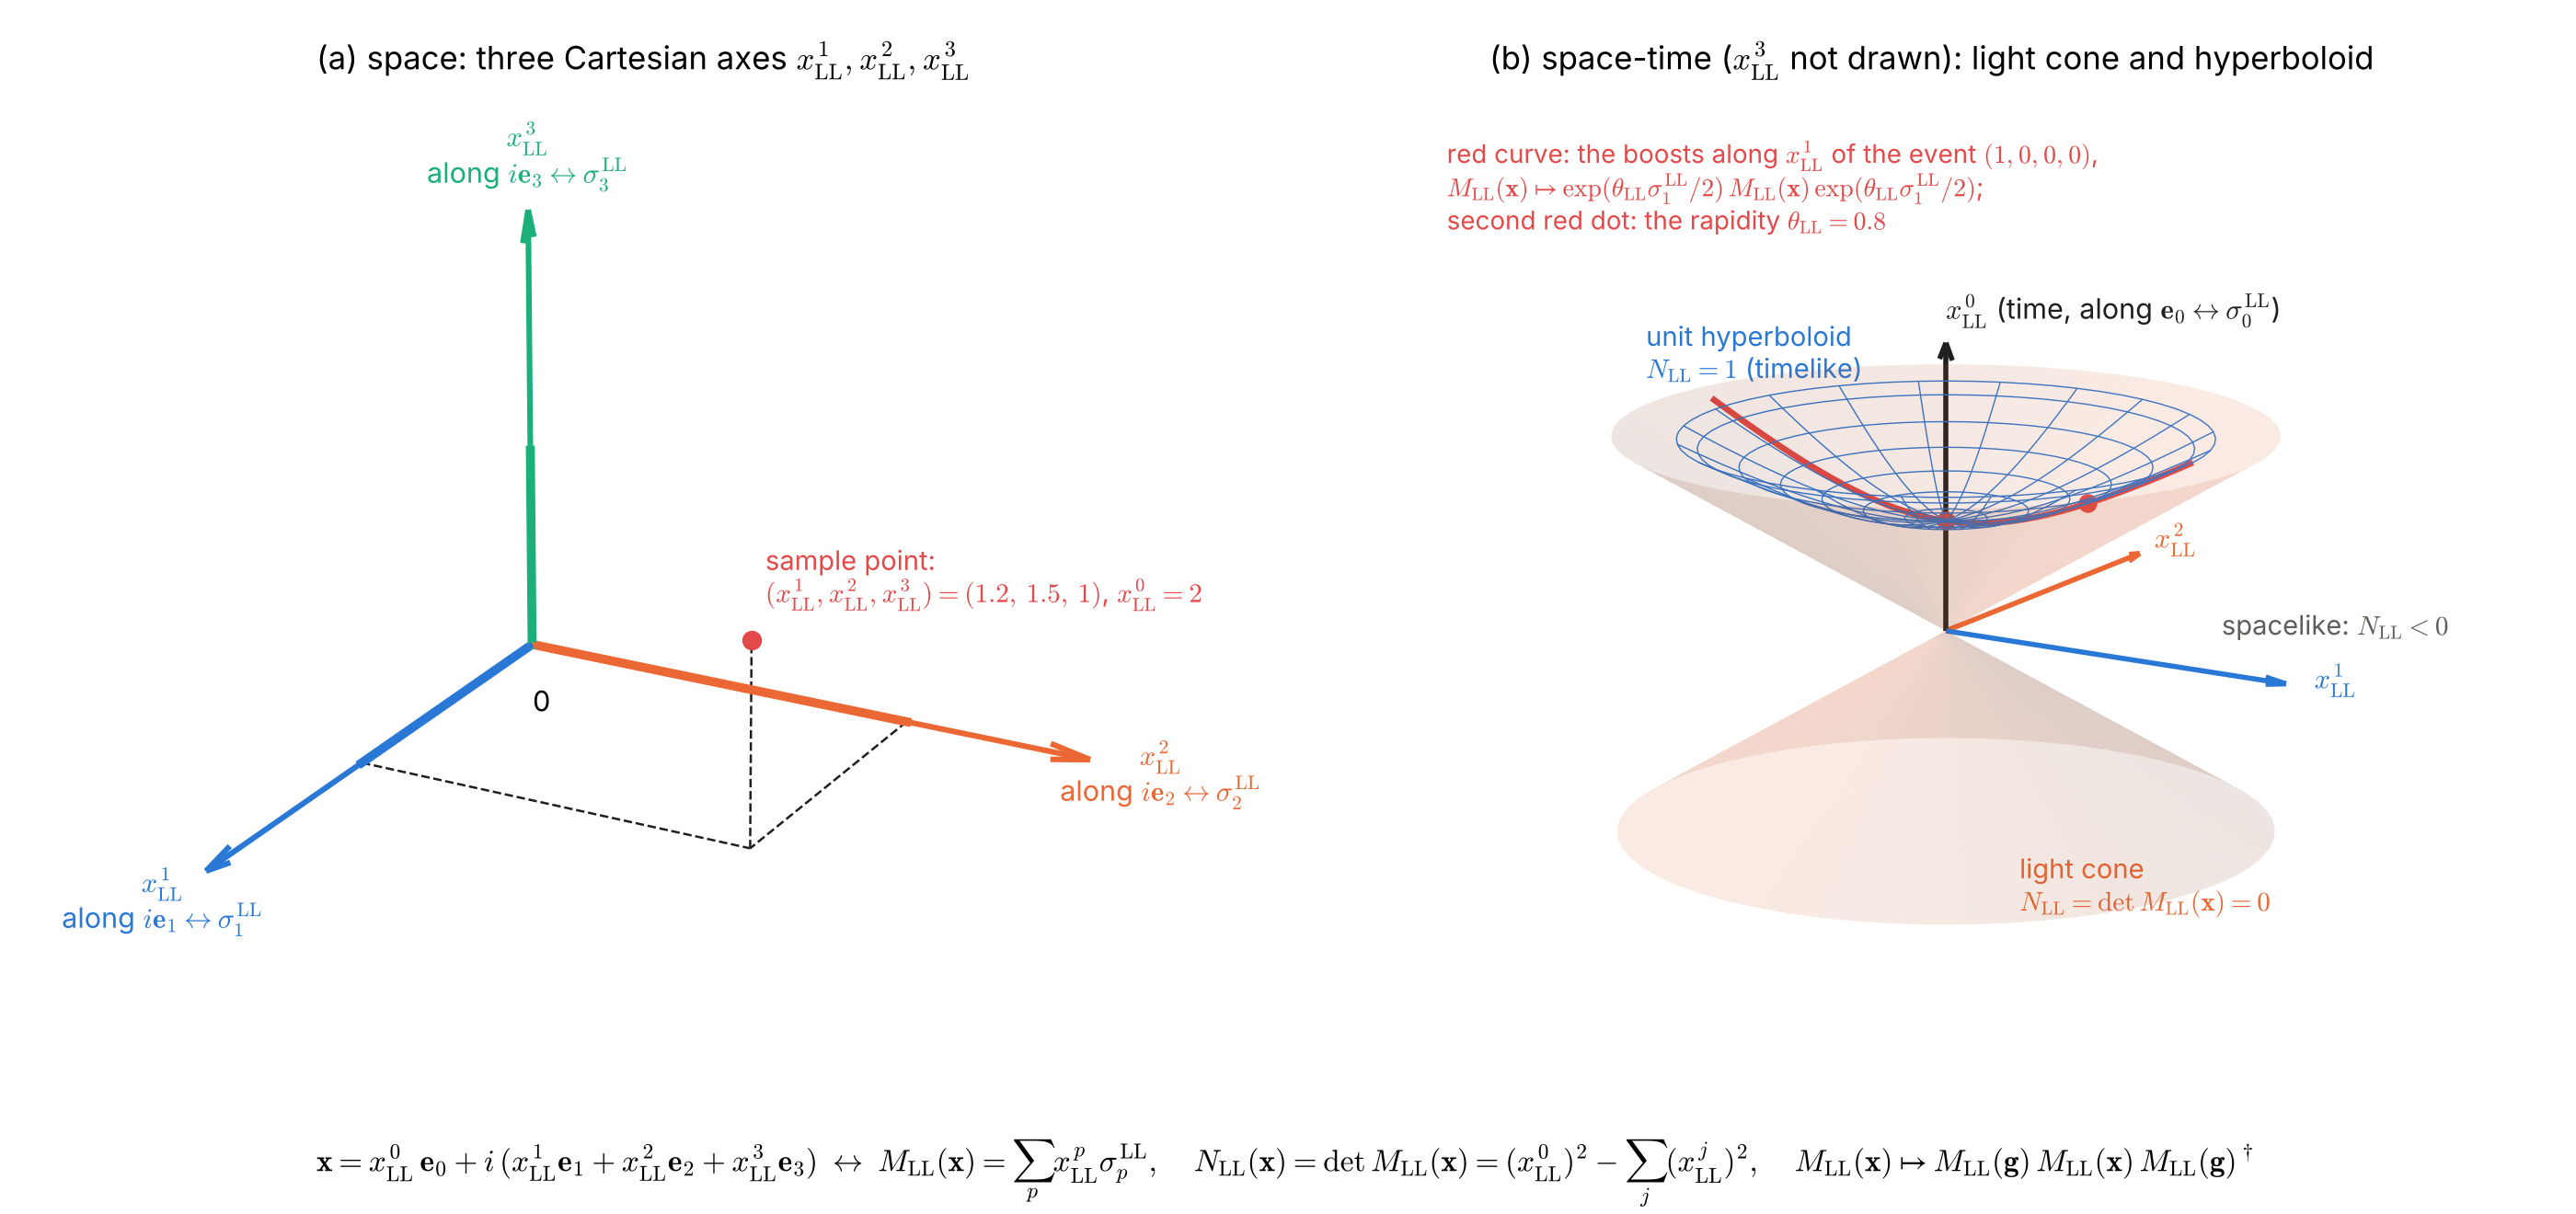
\includegraphics[width=1\textwidth,height=\textheight]{figures/fig_ex_r13_coordinates.png}

\textbf{Figure 1.} The coordinates of \(\mathbb R^{1,3}_{\rm LL}\),
drawn like Cartesian coordinates.

\begin{itemize}
\tightlist
\item
  \textbf{(a) Space.} The three space axes \(x^1_{\rm LL}\),
  \(x^2_{\rm LL}\), \(x^3_{\rm LL}\) point along the basis elements
  \(i\mathbf e_1\), \(i\mathbf e_2\), \(i\mathbf e_3\), which correspond
  to \(\sigma^{\rm LL}_1\), \(\sigma^{\rm LL}_2\),
  \(\sigma^{\rm LL}_3\). The sample point is drawn with its projections
  onto the axes (thick segments) and onto the
  \((x^1_{\rm LL},x^2_{\rm LL})\) plane (dashed lines).
\item
  \textbf{(b) Space-time, with \(x^3_{\rm LL}\) not drawn.}

  \begin{itemize}
  \tightlist
  \item
    The time axis \(x^0_{\rm LL}\) points along \(\mathbf e_0\), which
    corresponds to \(\sigma^{\rm LL}_0\).
  \item
    The light cone (orange) is
    \(N_{\rm LL}=\det M_{\rm LL}(\mathbf x)=0\); outside it the points
    are spacelike.
  \item
    The blue wire frame is the future unit hyperboloid \(N_{\rm LL}=1\).
  \item
    The red curve is the orbit of the event \((1,0,0,0)\) under the
    boosts along \(x^1_{\rm LL}\) (Section 3.2). It lies on the
    hyperboloid. The second red dot is its image under the boost with
    the rapidity 0.8.
  \end{itemize}
\item
  \textbf{Bottom line:} the formulas of Sections 2 and 3.
\end{itemize}

Data: \texttt{explanations/data/ex\_r13\_points.csv} and
\texttt{ex\_r13\_orbits.csv}; checks Z-1, Z-2, Z-5; drawn by
\texttt{explanations/code/make\_r13\_figures.py}.

\hypertarget{the-lorentz-group-on-the-manifold-comes-from-the-super-loop}{%
\section{3. The Lorentz group on the manifold comes from the
super-loop}\label{the-lorentz-group-on-the-manifold-comes-from-the-super-loop}}

\hypertarget{the-action-of-the-unit-bi-quaternions}{%
\subsection{3.1 The action of the unit
bi-quaternions}\label{the-action-of-the-unit-bi-quaternions}}

A unit bi-quaternion \(\mathbf g\) of the super-loop acts on
\(\mathbb R^{1,3}_{\rm LL}\) by
\[\mathbf x\longmapsto\mathbf g\,\mathbf x\,\mathbf g^\dagger,\qquad\text{that is}\qquad M_{\rm LL}(\mathbf x)\longmapsto M_{\rm LL}(\mathbf g)\,M_{\rm LL}(\mathbf x)\,M_{\rm LL}(\mathbf g)^\dagger. \tag{3.1}\]
Two lines show that this is a Lorentz transformation:

\begin{itemize}
\tightlist
\item
  \textbf{It maps the manifold to itself.} The image is again Hermitian:
  \((M_{\rm LL}(\mathbf g)M_{\rm LL}(\mathbf x)M_{\rm LL}(\mathbf g)^\dagger)^\dagger=M_{\rm LL}(\mathbf g)M_{\rm LL}(\mathbf x)^\dagger M_{\rm LL}(\mathbf g)^\dagger=M_{\rm LL}(\mathbf g)M_{\rm LL}(\mathbf x)M_{\rm LL}(\mathbf g)^\dagger\).
\item
  \textbf{It preserves the interval.} By the product rule of
  determinants,
  \(\det(M_{\rm LL}(\mathbf g)M_{\rm LL}(\mathbf x)M_{\rm LL}(\mathbf g)^\dagger)=\lvert\det M_{\rm LL}(\mathbf g)\rvert^2\det M_{\rm LL}(\mathbf x)=N_{\rm LL}(\mathbf x)\).
\end{itemize}

In the coordinates, Eq. (3.1) is a real \(4\times4\) matrix
\(\mathsf L_{\rm LL}(\mathbf g)\). Its entry in row \(p\) and column
\(p'\) is
\[\tfrac12\,\mathrm{Re}\,\mathrm{tr}\big(\sigma^{\rm LL}_pM_{\rm LL}(\mathbf g)\,\sigma^{\rm LL}_{p'}M_{\rm LL}(\mathbf g)^\dagger\big),\]
the \(p\)-th coordinate of the image of the \(p'\)-th basis element.
Check Z-3 verifies, for 200 random unit bi-quaternions \(\mathbf g\) and
\(\mathbf h\), that:

\begin{itemize}
\tightlist
\item
  \(\mathsf L_{\rm LL}(\mathbf g)\) keeps the metric:
  \(\mathsf L_{\rm LL}(\mathbf g)^T\,\mathrm{diag}(1,-1,-1,-1)\,\mathsf L_{\rm LL}(\mathbf g)=\mathrm{diag}(1,-1,-1,-1)\);
\item
  it has determinant 1, and its time-time entry is at least 1, so that
  it does not reverse the direction of time: it is a \textbf{proper
  orthochronous Lorentz transformation};
\item
  \(\mathbf g\) and \(-\mathbf g\) give the same \(\mathsf L_{\rm LL}\);
\item
  \(\mathsf L_{\rm LL}(\mathbf g\mathbf h)=\mathsf L_{\rm LL}(\mathbf g)\mathsf L_{\rm LL}(\mathbf h)\):
  the map from \(SL(2,\mathbb C)\) to the Lorentz group is a group
  homomorphism.
\end{itemize}

\textbf{Exactly two elements for each transformation.} If
\(\mathsf L_{\rm LL}(\mathbf g)\) is the unit matrix, then
\(M_{\rm LL}(\mathbf g)\) commutes with every Hermitian matrix: the
image of \(\mathbf e_0\) gives
\(M_{\rm LL}(\mathbf g)M_{\rm LL}(\mathbf g)^\dagger=\sigma^{\rm LL}_0\),
so \(M_{\rm LL}(\mathbf g)\) is unitary, and then
\(M_{\rm LL}(\mathbf g)\sigma^{\rm LL}_jM_{\rm LL}(\mathbf g)^{-1}=\sigma^{\rm LL}_j\)
for every \(j\). Only multiples of \(\sigma^{\rm LL}_0\) commute with
all three Pauli matrices, and the determinant 1 leaves
\(\pm\sigma^{\rm LL}_0\). So exactly \(\mathbf g\) and \(-\mathbf g\)
give the same transformation: \(SL(2,\mathbb C)\) is the \textbf{double
cover} of the Lorentz group. That every proper orthochronous Lorentz
transformation is reached is shown at the end of Section 3.2.

\hypertarget{rotations-and-boosts-and-their-generators-in-the-super-loop}{%
\subsection{3.2 Rotations and boosts, and their generators in the
super-loop}\label{rotations-and-boosts-and-their-generators-in-the-super-loop}}

The super-loop contains the \textbf{rotation generators}
\(J^j_{\rm LL}=\tfrac12\mathbf e_j\) and the \textbf{boost generators}
\(K^j_{\rm LL}=\tfrac12i\,\mathbf e_j\), with
\(M_{\rm LL}(J^j_{\rm LL})=-\tfrac i2\sigma^{\rm LL}_j\) and
\(M_{\rm LL}(K^j_{\rm LL})=\tfrac12\sigma^{\rm LL}_j\). Their
exponentials are the finite transformations; the real parameter
\(\theta_{\rm LL}\) is an angle for a rotation and a rapidity for a
boost.

\textbf{The rotation about the axis \(x^3_{\rm LL}\)} by the angle
\(\theta_{\rm LL}\) is \(\mathbf g=\exp(\theta_{\rm LL}J^3_{\rm LL})\),
with
\(M_{\rm LL}(\mathbf g)=\exp(-i\theta_{\rm LL}\sigma^{\rm LL}_3/2)\). It
gives
\[\mathsf L_{\rm LL}(\mathbf g)=\begin{pmatrix}1&0&0&0\\0&\cos\theta_{\rm LL}&-\sin\theta_{\rm LL}&0\\0&\sin\theta_{\rm LL}&\cos\theta_{\rm LL}&0\\0&0&0&1\end{pmatrix},\]
because
\(\exp(-i\theta_{\rm LL}\sigma^{\rm LL}_3/2)\,\sigma^{\rm LL}_1\,\exp(i\theta_{\rm LL}\sigma^{\rm LL}_3/2)=\sigma^{\rm LL}_1\exp(i\theta_{\rm LL}\sigma^{\rm LL}_3)=\cos\theta_{\rm LL}\,\sigma^{\rm LL}_1+\sin\theta_{\rm LL}\,\sigma^{\rm LL}_2\).
(The first step uses that \(\sigma^{\rm LL}_1\) anticommutes with
\(\sigma^{\rm LL}_3\); the second uses
\(i\sigma^{\rm LL}_1\sigma^{\rm LL}_3=\sigma^{\rm LL}_2\).) The matrices
\(\sigma^{\rm LL}_0\) and \(\sigma^{\rm LL}_3\) commute with
\(\sigma^{\rm LL}_3\) and stay fixed.

\textbf{The boost along the axis \(x^1_{\rm LL}\)} with the rapidity
\(\theta_{\rm LL}\) is \(\mathbf g=\exp(\theta_{\rm LL}K^1_{\rm LL})\),
with \(M_{\rm LL}(\mathbf g)=\exp(\theta_{\rm LL}\sigma^{\rm LL}_1/2)\),
a Hermitian matrix. It gives
\[\mathsf L_{\rm LL}(\mathbf g)=\begin{pmatrix}\cosh\theta_{\rm LL}&\sinh\theta_{\rm LL}&0&0\\\sinh\theta_{\rm LL}&\cosh\theta_{\rm LL}&0&0\\0&0&1&0\\0&0&0&1\end{pmatrix},\]
because
\(\exp(\theta_{\rm LL}\sigma^{\rm LL}_1/2)\,\sigma^{\rm LL}_0\,\exp(\theta_{\rm LL}\sigma^{\rm LL}_1/2)=\exp(\theta_{\rm LL}\sigma^{\rm LL}_1)=\cosh\theta_{\rm LL}\,\sigma^{\rm LL}_0+\sinh\theta_{\rm LL}\,\sigma^{\rm LL}_1\),
and \(\sigma^{\rm LL}_1\) goes to
\(\sigma^{\rm LL}_1\exp(\theta_{\rm LL}\sigma^{\rm LL}_1)=\sinh\theta_{\rm LL}\,\sigma^{\rm LL}_0+\cosh\theta_{\rm LL}\,\sigma^{\rm LL}_1\).
A boost mixes time with space, along hyperbolas; a rotation mixes two
space coordinates, along circles.

\textbf{A rotation by \(2\pi\)} has
\(M_{\rm LL}(\mathbf g)=\exp(-i\pi\sigma^{\rm LL}_3)=-\sigma^{\rm LL}_0\),
and \(\mathsf L_{\rm LL}(\mathbf g)\) is the unit matrix: every point
returns to itself, while the group element is \(-1\).

\textbf{The generators.} For a generator \(\mathbf u\)
(\(\mathbf u=J^j_{\rm LL}\) or \(K^j_{\rm LL}\)) and
\(\mathbf g=\exp(\theta_{\rm LL}\mathbf u)\), the derivative of Eq.
(3.1) at \(\theta_{\rm LL}=0\) is the infinitesimal transformation
\[\mathbf x\longmapsto\mathbf u\mathbf x+\mathbf x\mathbf u^\dagger,\qquad M_{\rm LL}(\mathbf x)\longmapsto M_{\rm LL}(\mathbf u)M_{\rm LL}(\mathbf x)+M_{\rm LL}(\mathbf x)M_{\rm LL}(\mathbf u)^\dagger .\]
Its real \(4\times4\) matrix in the coordinates is
\(\mathcal V_{\rm LL}(\mathbf u)\), the \textbf{vector action} of
\(\mathbf u\). The six matrices \(\mathcal V_{\rm LL}(J^j_{\rm LL})\)
and \(\mathcal V_{\rm LL}(K^j_{\rm LL})\) have three properties:

\begin{itemize}
\tightlist
\item
  they are linearly independent;
\item
  they preserve the metric:
  \(\mathcal V_{\rm LL}(\mathbf u)^T\mathrm{diag}(1,-1,-1,-1)+\mathrm{diag}(1,-1,-1,-1)\,\mathcal V_{\rm LL}(\mathbf u)=0\);
\item
  they obey the commutation relations of the Lorentz algebra
  \(\mathfrak{so}(3,1)\).
\end{itemize}

The third property follows from the generators themselves. Expanding the
two products gives
\[\mathcal V_{\rm LL}(\mathbf u)\mathcal V_{\rm LL}(\mathbf u')\mathbf x-\mathcal V_{\rm LL}(\mathbf u')\mathcal V_{\rm LL}(\mathbf u)\mathbf x=[\mathbf u,\mathbf u']\,\mathbf x+\mathbf x\,[\mathbf u,\mathbf u']^\dagger,\]
where
\([\mathbf u,\mathbf u']=\mathbf u\mathbf u'-\mathbf u'\mathbf u\); the
mixed terms \(\mathbf u\mathbf x\mathbf u'^\dagger\) and
\(\mathbf u'\mathbf x\mathbf u^\dagger\) cancel. So the commutators of
the six matrices are the matrices of the commutators of the generators,
and these are
\[[J^j_{\rm LL},J^{j'}_{\rm LL}]=\sum_{j''}\epsilon^{\rm LL}_{jj'j''}J^{j''}_{\rm LL},\qquad[J^j_{\rm LL},K^{j'}_{\rm LL}]=\sum_{j''}\epsilon^{\rm LL}_{jj'j''}K^{j''}_{\rm LL},\qquad[K^j_{\rm LL},K^{j'}_{\rm LL}]=-\sum_{j''}\epsilon^{\rm LL}_{jj'j''}J^{j''}_{\rm LL}, \tag{3.2}\]
with the Levi-Civita symbol \(\epsilon^{\rm LL}_{jj'j''}\) (\(+1\) for
an even permutation of \(1,2,3\), \(-1\) for an odd one, 0 otherwise).
For example,
\([J^1_{\rm LL},J^2_{\rm LL}]=\tfrac14(\mathbf e_1\mathbf e_2-\mathbf e_2\mathbf e_1)=\tfrac12\mathbf e_3=J^3_{\rm LL}\)
and
\([K^1_{\rm LL},K^2_{\rm LL}]=\tfrac14i^2(\mathbf e_1\mathbf e_2-\mathbf e_2\mathbf e_1)=-J^3_{\rm LL}\).
The minus sign in the last relation distinguishes the Lorentz algebra
from the algebra \(\mathfrak{so}(4)\) of the rotations of
four-dimensional Euclidean space: two boosts in different directions
combine into a rotation (the Thomas precession). Check Z-4 verifies all
27 relations on the \(4\times4\) matrices, their linear independence,
the preservation of the metric, and that the derivatives of the finite
transformations at \(\theta_{\rm LL}=0\) equal the generators.

\textbf{Every proper orthochronous Lorentz transformation is reached.}
The six independent matrices span the whole six-dimensional Lorentz
algebra. So the transformations \(\mathsf L_{\rm LL}(\mathbf g)\) fill a
neighbourhood of the unit matrix in the Lorentz group. The group of
proper orthochronous Lorentz transformations is connected, and every
element of a connected group is a product of elements from any
neighbourhood of the unit element. Because \(\mathsf L_{\rm LL}\) is a
homomorphism, every proper orthochronous Lorentz transformation is
therefore \(\mathsf L_{\rm LL}(\mathbf g)\) for some unit bi-quaternion
\(\mathbf g\), and by Section 3.1 for exactly two, \(\pm\mathbf g\).

(In the \(7+1\) space \(\mathbb R^{1,7}_{\rm LL}\) the same six
generators do not close: their Lie closure there has dimension 9.
\(\mathbb R^{1,3}_{\rm LL}\) is the part of the bi-octonions on which
the super-loop's own Lorentz generators act as an honest Lorentz group;
check N-5 of the program \texttt{superloop}, printed in Section 7.3.)

\textbf{Worked examples} (check Z-5; the table is written from the data
file \texttt{explanations/data/ex\_r13\_points.csv}):

\begin{longtable}[]{@{}
  >{\raggedright\arraybackslash}p{(\columnwidth - 12\tabcolsep) * \real{0.3200}}
  >{\raggedright\arraybackslash}p{(\columnwidth - 12\tabcolsep) * \real{0.0900}}
  >{\raggedright\arraybackslash}p{(\columnwidth - 12\tabcolsep) * \real{0.0900}}
  >{\raggedright\arraybackslash}p{(\columnwidth - 12\tabcolsep) * \real{0.0900}}
  >{\raggedright\arraybackslash}p{(\columnwidth - 12\tabcolsep) * \real{0.0900}}
  >{\raggedright\arraybackslash}p{(\columnwidth - 12\tabcolsep) * \real{0.1200}}
  >{\raggedright\arraybackslash}p{(\columnwidth - 12\tabcolsep) * \real{0.2000}}@{}}
\toprule\noalign{}
\begin{minipage}[b]{\linewidth}\raggedright
example
\end{minipage} & \begin{minipage}[b]{\linewidth}\raggedright
\(x^0_{\rm LL}\)
\end{minipage} & \begin{minipage}[b]{\linewidth}\raggedright
\(x^1_{\rm LL}\)
\end{minipage} & \begin{minipage}[b]{\linewidth}\raggedright
\(x^2_{\rm LL}\)
\end{minipage} & \begin{minipage}[b]{\linewidth}\raggedright
\(x^3_{\rm LL}\)
\end{minipage} & \begin{minipage}[b]{\linewidth}\raggedright
\(N_{\rm LL}(\mathbf x)\)
\end{minipage} & \begin{minipage}[b]{\linewidth}\raggedright
kind
\end{minipage} \\
\midrule\noalign{}
\endhead
\bottomrule\noalign{}
\endlastfoot
the sample point & 2.000000 & 1.200000 & 1.500000 & 1.000000 &
\(-0.690000\) & spacelike \\
the event \((1,0,0,0)\) & 1.000000 & 0 & 0 & 0 & 1.000000 & timelike \\
after the boost along \(x^1_{\rm LL}\) with the rapidity 0.8 & 1.337435
& 0.888106 & 0 & 0 & 1.000000 & timelike \\
the event \((0,1,0,0)\) & 0 & 1.000000 & 0 & 0 & \(-1.000000\) &
spacelike \\
after the rotation about \(x^3_{\rm LL}\) by the angle \(\pi/3\) & 0 &
0.500000 & 0.866025 & 0 & \(-1.000000\) & spacelike \\
the point \(\chi_{\rm LL}\chi_{\rm LL}^\dagger\) of
\(\chi_{\rm LL}=(1,0)\) & 0.500000 & 0 & 0 & 0.500000 & 0 & null (on the
light cone) \\
after the boost of \(\chi_{\rm LL}\) along \(x^3_{\rm LL}\) with the
rapidity 0.8 & 1.112770 & 0 & 0 & 1.112770 & 0 & null (on the light
cone) \\
\end{longtable}

The boost with the rapidity 0.8 takes \((1,0,0,0)\) to
\((\cosh0.8,\sinh0.8,0,0)\) and keeps \(N_{\rm LL}=1\). The rotation by
\(\pi/3\) takes \((0,1,0,0)\) to \((0,\tfrac12,\tfrac{\sqrt3}2,0)\) and
keeps \(N_{\rm LL}=-1\). Figure 2 shows these transformations as curves.

\hypertarget{spinors-on-the-manifold-and-the-spinor-charges}{%
\subsection{3.3 Spinors on the manifold, and the spinor
charges}\label{spinors-on-the-manifold-and-the-spinor-charges}}

A \textbf{two-component spinor} \(\chi_{\rm LL}\) is a column of two
complex numbers. It transforms under the unit bi-quaternion
\(\mathbf g\) as
\(\chi_{\rm LL}\mapsto M_{\rm LL}(\mathbf g)\chi_{\rm LL}\). Two facts
tie such spinors to the manifold:

\begin{itemize}
\tightlist
\item
  \textbf{A spinor gives a point on the light cone.} The Hermitian
  matrix \(\chi_{\rm LL}\chi_{\rm LL}^\dagger\) is the matrix of a point
  of \(\mathbb R^{1,3}_{\rm LL}\). It has determinant 0 (its rank is 1)
  and the positive trace \(\lvert\chi_{\rm LL}\rvert^2\), so the point
  lies on the \textbf{future light cone}. Under \(\mathbf g\) it
  transforms by Eq. (3.1), because
  \((M_{\rm LL}(\mathbf g)\chi_{\rm LL})(M_{\rm LL}(\mathbf g)\chi_{\rm LL})^\dagger=M_{\rm LL}(\mathbf g)\,\chi_{\rm LL}\chi_{\rm LL}^\dagger\,M_{\rm LL}(\mathbf g)^\dagger\).
  A spinor is thus a ``square root'' of a light ray.
\item
  \textbf{The double cover becomes visible.} A rotation by \(2\pi\)
  changes the sign of \(\chi_{\rm LL}\), but it leaves the point
  \(\chi_{\rm LL}\chi_{\rm LL}^\dagger\) unchanged.
\end{itemize}

\emph{Example.} \(\chi_{\rm LL}=(1,0)\) gives
\(\chi_{\rm LL}\chi_{\rm LL}^\dagger=\mathrm{diag}(1,0)=\tfrac12(\sigma^{\rm LL}_0+\sigma^{\rm LL}_3)\),
the null point \((\tfrac12,0,0,\tfrac12)\). The boost along
\(x^3_{\rm LL}\) with the rapidity 0.8,
\(M_{\rm LL}(\mathbf g)=\exp(0.4\,\sigma^{\rm LL}_3)\), multiplies
\(\chi_{\rm LL}\) by \(\exp(0.4)\) and the null point by \(\exp(0.8)\).
The point moves along the light cone: this is the Doppler shift of a
light ray (Figure 2(c)).

\textbf{The spinor charges are such spinors.} A spinor charge of the
super-loop is a bi-octonion \(\mathbf b\,\mathbf e_4\) with a
bi-quaternion \(\mathbf b\). The Lorentz transformations of the
super-loop act on it by multiplying \(\mathbf b\) from the right: the
infinitesimal transformation generated by \(\mathbf u\) multiplies
\(\mathbf b\) by \(-\mathbf u\) from the right, so the finite
transformation by \(\mathbf g=\exp(\theta_{\rm LL}\mathbf u)\) changes
\(\mathbf b\) into \(\mathbf b\bar{\mathbf g}\) (for these generators
\(\bar{\mathbf u}=-\mathbf u\), so
\(\bar{\mathbf g}=\exp(-\theta_{\rm LL}\mathbf u)\)). The \textbf{Weyl
isodoublet} of the spinor charge is the \(2\times2\) matrix
\[\psi'_{\rm LL}=\mathsf E_{\rm LL}^{-1}M_{\rm LL}(\mathbf b)^T,\qquad\mathsf E_{\rm LL}=i\sigma^{\rm LL}_2=\begin{pmatrix}0&1\\-1&0\end{pmatrix}.\]
Its first column is the isospin-up component and its second column the
isospin-down component. Under \(\mathbf g\), \(M_{\rm LL}(\mathbf b)^T\)
becomes \(M_{\rm LL}(\bar{\mathbf g})^TM_{\rm LL}(\mathbf b)^T\), so
each column transforms as
\[\chi_{\rm LL}\longmapsto\mathsf E_{\rm LL}^{-1}M_{\rm LL}(\bar{\mathbf g})^T\mathsf E_{\rm LL}\,\chi_{\rm LL}=M_{\rm LL}(\mathbf g)\,\chi_{\rm LL}.\]
The last equality holds for every unit bi-quaternion. Multiplying out
the four entries shows that
\(M_{\rm LL}(\mathbf b)^T\mathsf E_{\rm LL}M_{\rm LL}(\mathbf b)=N_{\rm LL}(\mathbf b)\,\mathsf E_{\rm LL}\)
for every bi-quaternion \(\mathbf b\). With \(\bar{\mathbf g}\) in place
of \(\mathbf b\) (norm 1) this gives
\(\mathsf E_{\rm LL}^{-1}M_{\rm LL}(\bar{\mathbf g})^T\mathsf E_{\rm LL}=M_{\rm LL}(\bar{\mathbf g})^{-1}=M_{\rm LL}(\mathbf g)\)
(check Z-5, 200 random cases).

So \textbf{the spinor charges are two-component spinors of the Lorentz
group of \(\mathbb R^{1,3}_{\rm LL}\), each with an isospin label}, and
the generators act on them as
\(M_{\rm LL}(J^j_{\rm LL})=-\tfrac i2\sigma^{\rm LL}_j\) and
\(M_{\rm LL}(K^j_{\rm LL})=\tfrac12\sigma^{\rm LL}_j\). Their quantum
field, the Dirac isodoublet \(\Psi_{\rm LL}\) of Section 4, is a
function of the point \(\mathbf x\) of \(\mathbb R^{1,3}_{\rm LL}\).
This is the precise sense in which the theory of the spinor charges
``lives'' on the \(3+1\) manifold.

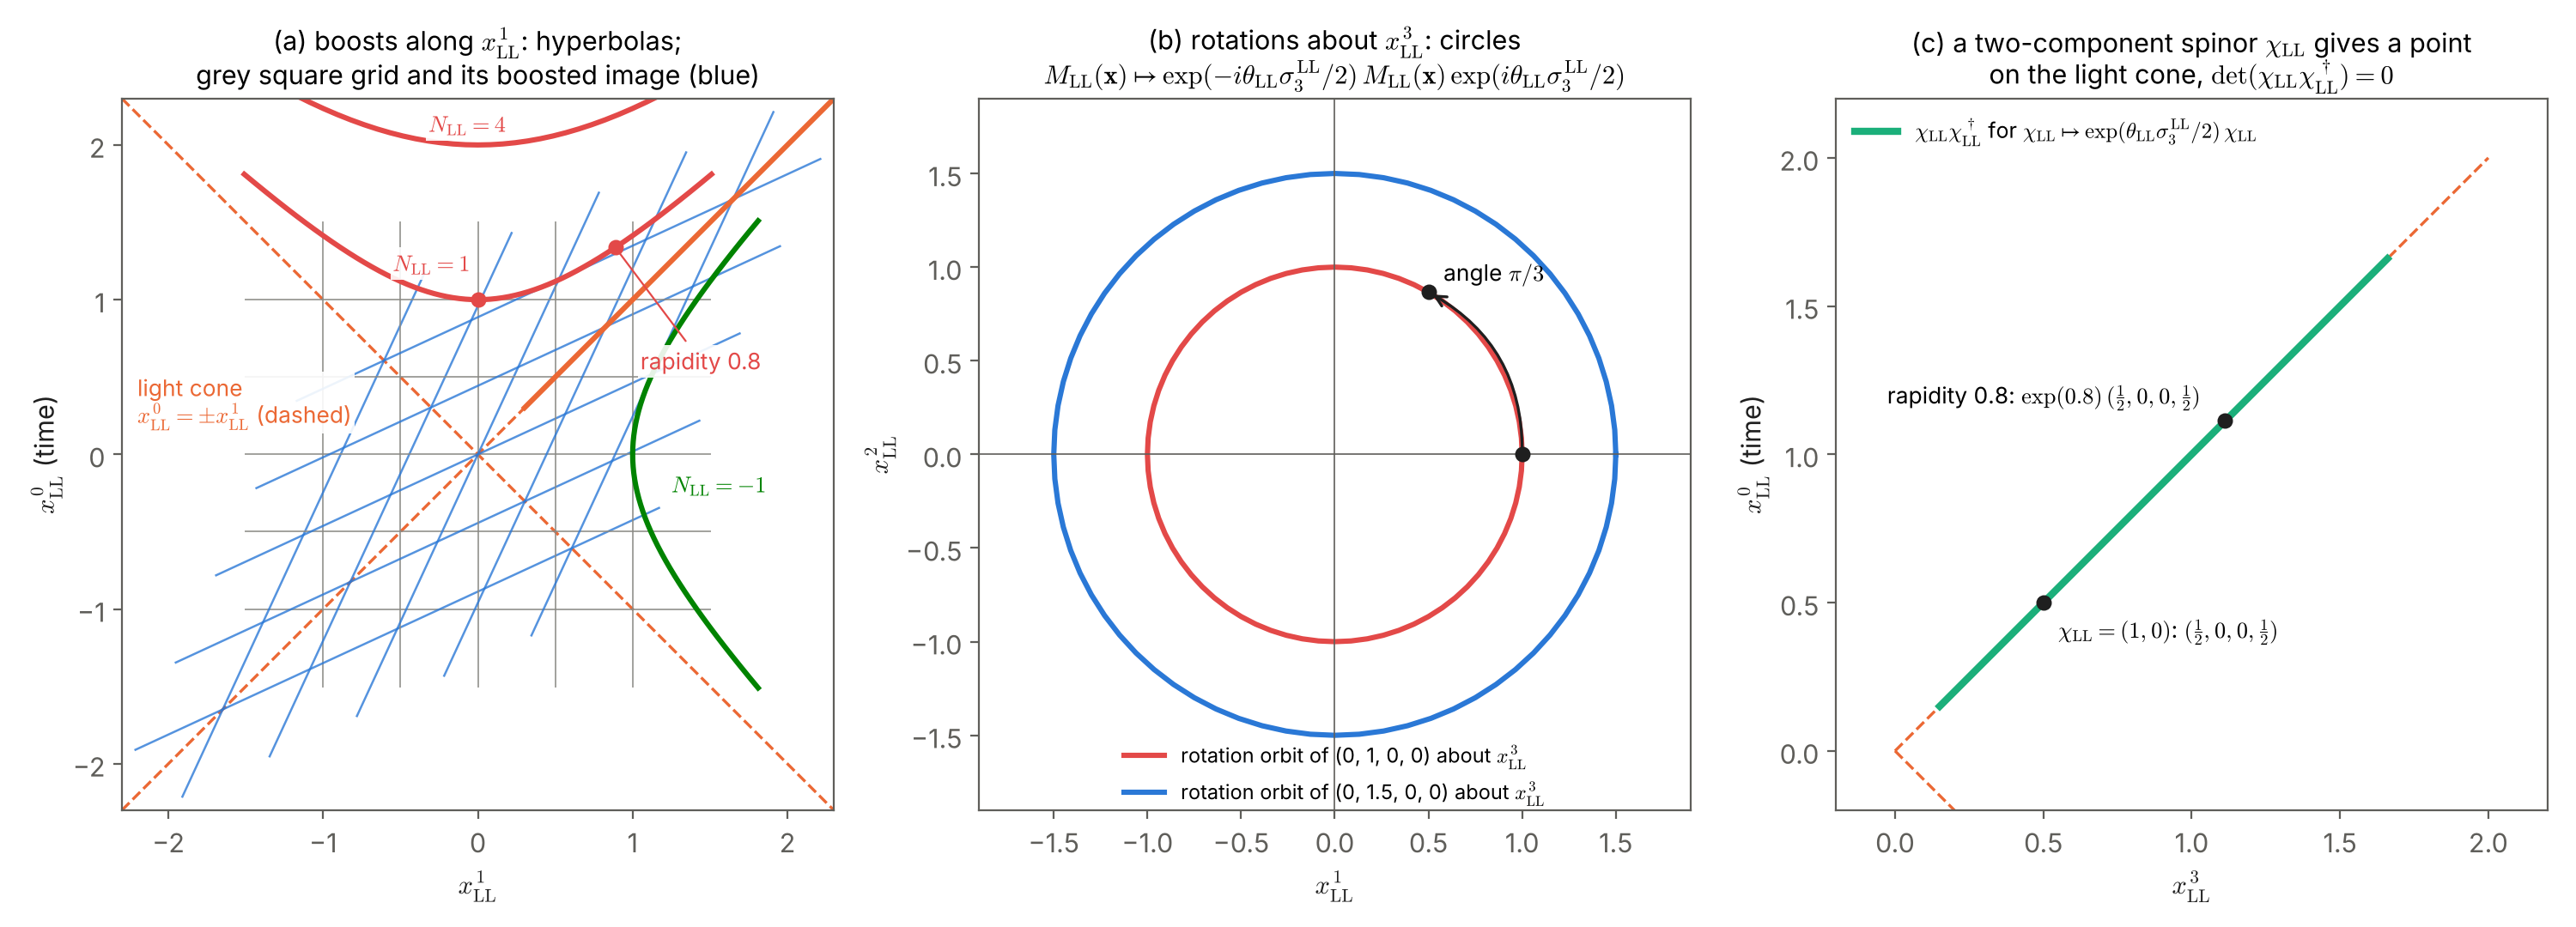
\includegraphics[width=1\textwidth,height=\textheight]{figures/fig_ex_r13_lorentz.png}

\textbf{Figure 2.} The Lorentz transformations of
\(\mathbb R^{1,3}_{\rm LL}\), computed from Eq. (3.1).

\begin{itemize}
\tightlist
\item
  \textbf{(a) Boosts along \(x^1_{\rm LL}\), in the
  \((x^1_{\rm LL},x^0_{\rm LL})\) plane.}

  \begin{itemize}
  \tightlist
  \item
    The orbits of the events \((1,0,0,0)\) and \((2,0,0,0)\) (red) are
    the hyperbolas \(N_{\rm LL}=1\) and \(N_{\rm LL}=4\). The red dots
    are \((1,0,0,0)\) and its image under the boost with the rapidity
    0.8.
  \item
    The orbit of \((0,1,0,0)\) (green) is the hyperbola
    \(N_{\rm LL}=-1\).
  \item
    The orbit of the null event \((1,1,0,0)\) (orange, solid) stays on
    the light cone (orange, dashed).
  \item
    A grey square grid is drawn with its image under the boost with the
    rapidity 0.5 (blue). The boost shears the grid along the light cone
    and leaves the light cone in place.
  \end{itemize}
\item
  \textbf{(b) Rotations about \(x^3_{\rm LL}\), in the
  \((x^1_{\rm LL},x^2_{\rm LL})\) plane.} The orbits of \((0,1,0,0)\)
  (red) and \((0,1.5,0,0)\) (blue) are circles. The arrow is the
  rotation by \(\pi/3\) of the example.
\item
  \textbf{(c) The null points of the spinor \(\chi_{\rm LL}=(1,0)\), in
  the \((x^3_{\rm LL},x^0_{\rm LL})\) plane.} As \(\chi_{\rm LL}\) is
  boosted along \(x^3_{\rm LL}\), its null point
  \(\chi_{\rm LL}\chi_{\rm LL}^\dagger\) (green) moves along the light
  cone (dashed). The black dots are the two points of the example.
\end{itemize}

Data: \texttt{explanations/data/ex\_r13\_orbits.csv} and
\texttt{ex\_r13\_points.csv}; checks Z-3 to Z-5; drawn by
\texttt{explanations/code/make\_r13\_figures.py}.

\hypertarget{the-field-theory-on-the-manifold-the-contact-form-and-the-yukawa-form}{%
\section{4. The field theory on the manifold: the contact form and the
Yukawa
form}\label{the-field-theory-on-the-manifold-the-contact-form-and-the-yukawa-form}}

\hypertarget{the-fields}{%
\subsection{4.1 The fields}\label{the-fields}}

Two fields are functions of the point \(\mathbf x\) of
\(\mathbb R^{1,3}_{\rm LL}\); \(\partial_p\) is the derivative with
respect to \(x^p_{\rm LL}\).

\textbf{The spinor charges: the field \(\Psi_{\rm LL}\).} The Dirac
matrices in the chiral basis are
\[\gamma^0_{\rm LL}=\begin{pmatrix}0&\sigma^{\rm LL}_0\\\sigma^{\rm LL}_0&0\end{pmatrix},\qquad\gamma^j_{\rm LL}=\begin{pmatrix}0&\sigma^{\rm LL}_j\\-\sigma^{\rm LL}_j&0\end{pmatrix},\]
with the chirality matrix
\(\gamma^{\rm ch}_{\rm LL}=i\gamma^0_{\rm LL}\gamma^1_{\rm LL}\gamma^2_{\rm LL}\gamma^3_{\rm LL}=\mathrm{diag}(-1,-1,1,1)\)
and the charge-conjugation matrix
\(C_{\rm LL}=i\gamma^2_{\rm LL}\gamma^0_{\rm LL}=\mathrm{diag}(\mathsf E_{\rm LL},-\mathsf E_{\rm LL})\).

\begin{itemize}
\tightlist
\item
  The spinor charges, on which the boosts act as
  \(+\tfrac12\sigma^{\rm LL}_j\) (Section 3.3), are the lower block of a
  Dirac spinor (\(\gamma^{\rm ch}_{\rm LL}=+1\)).
\item
  The complex-conjugate super-loop, on which the boosts act with the
  opposite sign, supplies the upper block.
\item
  The field of the spinor charges is therefore a \textbf{Dirac
  isodoublet} \(\Psi_{\rm LL}\) with eight components (four Dirac
  components times two isospin components).
\item
  Its electric charges are \(Q_{\rm LL}=\pm\tfrac12\), where
  \(Q_{\rm LL}=T^3_{\rm LL}\) and \(T^\iota_{\rm LL}\) are the isospin
  generators.
\item
  Its components have spinor number \(-1\): they change sign under the
  rotation by \(2\pi\). By the spin-statistics theorem,
  \(\Psi_{\rm LL}\) is therefore a fermion field, and its components
  anticommute.
\end{itemize}

The Dirac adjoint is
\(\bar\Psi_{\rm LL}=\Psi^\dagger_{\rm LL}\gamma^0_{\rm LL}\).

\textbf{The spin-zero pairs.} A pair of two spinor charges at the same
point is \(\Psi^T_{\rm LL}\mathsf K\Psi_{\rm LL}\) with an \(8\times8\)
matrix \(\mathsf K\). Because the components anticommute, only the
antisymmetric part of \(\mathsf K\) contributes. The antisymmetric
matrices for which the pair is Lorentz invariant (spin zero) form a
complex space of dimension 6, spanned by
\[\mathsf K^\iota_{\rm LL}=C_{\rm LL}\gamma^{\rm ch}_{\rm LL}\otimes\mathsf E_{\rm LL}\tau^{\rm LL}_\iota\ \ (\text{scalar, }0^+),\qquad\mathsf K'^\iota_{\rm LL}=C_{\rm LL}\otimes\mathsf E_{\rm LL}\tau^{\rm LL}_\iota\ \ (\text{pseudoscalar, }0^-),\]
where \(\tau^{\rm LL}_\iota\) are the Pauli matrices acting on the
isospin index. The reason, in three steps:

\begin{enumerate}
\def\labelenumi{\arabic{enumi}.}
\tightlist
\item
  The Lorentz-invariant bilinear forms of a Dirac spinor are spanned by
  \(C_{\rm LL}\) and
  \(C_{\rm LL}\gamma^{\rm ch}_{\rm LL}=-\mathrm{diag}(\mathsf E_{\rm LL},\mathsf E_{\rm LL})\),
  one for each chirality block. Both are antisymmetric.
\item
  The whole matrix must be antisymmetric, so the isospin factor must be
  symmetric.
\item
  The symmetric \(2\times2\) matrices are spanned by the three matrices
  \(\mathsf E_{\rm LL}\tau^{\rm LL}_\iota\), which form an isospin
  vector. The remaining matrix \(\mathsf E_{\rm LL}\), the isosinglet,
  is antisymmetric and drops out.
\end{enumerate}

Every spin-zero pair is therefore an isospin \textbf{triplet}. The pair
\(\Psi^T_{\rm LL}\mathsf K^\iota_{\rm LL}\Psi_{\rm LL}\) has fermion
number 2: it annihilates two spinor charges.

\textbf{The pair field: the field \(\phi_{\rm LL}\).} This is a complex
isospin triplet
\(\phi_{\rm LL}=(\phi^1_{\rm LL},\phi^2_{\rm LL},\phi^3_{\rm LL})\), a
scalar field. It describes the scalar pairs as particles of their own.

\hypertarget{the-two-forms-of-the-theory}{%
\subsection{4.2 The two forms of the
theory}\label{the-two-forms-of-the-theory}}

\textbf{The contact form.} The spinor charges attract each other in the
scalar channel through a contact interaction of strength
\(G_{\rm LL}>0\):
\[\mathcal L^{\rm c}_{\rm LL}=\bar\Psi_{\rm LL}\Big(i\sum_p\gamma^p_{\rm LL}\partial_p-m_{\rm LL}\Big)\Psi_{\rm LL}+\tfrac14G_{\rm LL}\sum_\iota\big(\Psi^T_{\rm LL}\mathsf K^\iota_{\rm LL}\Psi_{\rm LL}\big)^\dagger\big(\Psi^T_{\rm LL}\mathsf K^\iota_{\rm LL}\Psi_{\rm LL}\big), \tag{4.1}\]
with the mass \(m_{\rm LL}\) of the spinor charges. Two remarks connect
it with the superfluid:

\begin{itemize}
\tightlist
\item
  At a chemical potential \(\mu_{\rm LL}\) the term
  \(\mu_{\rm LL}\Psi^\dagger_{\rm LL}\Psi_{\rm LL}\) is added. It is a
  term of dimension 3 with a coefficient of dimension 1 and changes no
  power counting.
\item
  The superfluid calculation keeps from this interaction only the pairs
  of total momentum zero (the reduced, or BCS, form of Eq. (4.1)). The
  power counting concerns the full local interaction (4.1).
\end{itemize}

\textbf{The Yukawa form.} The contact interaction is replaced by the
exchange of the pair field:
\[\begin{aligned}\mathcal L^{\rm Y}_{\rm LL}={}&\bar\Psi_{\rm LL}\Big(i\sum_p\gamma^p_{\rm LL}\partial_p-m_{\rm LL}\Big)\Psi_{\rm LL}+\sum_\iota\Big(\lvert\partial_0\phi^\iota_{\rm LL}\rvert^2-\sum_j\lvert\partial_j\phi^\iota_{\rm LL}\rvert^2-(m^\phi_{\rm LL})^2\lvert\phi^\iota_{\rm LL}\rvert^2\Big)\\&-g^{\rm Y}_{\rm LL}\sum_\iota\Big(\phi^{\iota*}_{\rm LL}\,\Psi^T_{\rm LL}\mathsf K^\iota_{\rm LL}\Psi_{\rm LL}+\text{h.c.}\Big)-\lambda^{(1)}_{\rm LL}\big(\phi^\dagger_{\rm LL}\phi_{\rm LL}\big)^2-\lambda^{(2)}_{\rm LL}\big\lvert\phi^T_{\rm LL}\phi_{\rm LL}\big\rvert^2 .\end{aligned} \tag{4.2}\]
Here h.c. is the Hermitian conjugate of the preceding term. The
parameters are:

\begin{itemize}
\tightlist
\item
  \(m^\phi_{\rm LL}\), the mass of the pair field;
\item
  \(g^{\rm Y}_{\rm LL}\), the Yukawa coupling;
\item
  \(\lambda^{(1)}_{\rm LL}\) and \(\lambda^{(2)}_{\rm LL}\), the two
  quartic couplings.
\end{itemize}

\textbf{The symmetries of both forms.} Both forms are invariant under:

\begin{itemize}
\tightlist
\item
  the Lorentz group of Section 3, with \(\Psi_{\rm LL}\) a Dirac spinor
  and \(\phi_{\rm LL}\) a scalar;
\item
  the isospin rotations \(SU(2)_{\rm v}\), generated by
  \(T^\iota_{\rm LL}\), with \(\phi_{\rm LL}\) a vector;
\item
  the fermion-number rotations
  \(\Psi_{\rm LL}\to\exp(i\theta_{\rm LL})\Psi_{\rm LL}\),
  \(\phi_{\rm LL}\to\exp(2i\theta_{\rm LL})\phi_{\rm LL}\), generated by
  the fermion number \(F_{\rm LL}\) (the pair field carries fermion
  number 2);
\item
  parity, with \(\phi_{\rm LL}\) a scalar of positive parity (\(0^+\)).
\end{itemize}

\hypertarget{the-yukawa-form-contains-the-contact-form}{%
\subsection{4.3 The Yukawa form contains the contact
form}\label{the-yukawa-form-contains-the-contact-form}}

At momenta much smaller than \(m^\phi_{\rm LL}\) the derivative terms of
\(\phi_{\rm LL}\) are negligible. The field \(\phi_{\rm LL}\) then
follows its equation of motion, obtained by varying Eq. (4.2) with
respect to \(\phi^{\iota*}_{\rm LL}\):
\[\phi^\iota_{\rm LL}=-\frac{g^{\rm Y}_{\rm LL}}{(m^\phi_{\rm LL})^2}\,\Psi^T_{\rm LL}\mathsf K^\iota_{\rm LL}\Psi_{\rm LL}\]
(the quartic terms are of higher order in the fields and are dropped
here). Inserted into Eq. (4.2), each term multiplies
\(\sum_\iota\lvert\Psi^T_{\rm LL}\mathsf K^\iota_{\rm LL}\Psi_{\rm LL}\rvert^2\):

\begin{itemize}
\tightlist
\item
  the mass term contributes
  \(-(g^{\rm Y}_{\rm LL})^2/(m^\phi_{\rm LL})^2\);
\item
  the Yukawa term contributes
  \(+2(g^{\rm Y}_{\rm LL})^2/(m^\phi_{\rm LL})^2\).
\end{itemize}

The result is exactly the contact form (4.1) with
\[G_{\rm LL}=\frac{4\,(g^{\rm Y}_{\rm LL})^2}{(m^\phi_{\rm LL})^2}. \tag{4.3}\]
The Yukawa form is therefore a completion of the contact form: it agrees
with it at low energies and resolves the contact interaction at high
energies. The mass dimensions of Section 5.1 are consistent with Eq.
(4.3): \(2[g^{\rm Y}_{\rm LL}]-2=(3-D)-2=1-D=[G_{\rm LL}]\) (check Z-6
verifies this for \(D=3\) and \(D=7\)).

\hypertarget{why-the-yukawa-form-is-renormalizable-in-31-dimensions}{%
\section{5. Why the Yukawa form is renormalizable in 3+1
dimensions}\label{why-the-yukawa-form-is-renormalizable-in-31-dimensions}}

\hypertarget{mass-dimensions}{%
\subsection{5.1 Mass dimensions}\label{mass-dimensions}}

In units with \(\hbar=1\) and the speed of light 1, every quantity has a
\textbf{mass dimension}, written with square brackets: a coordinate has
the dimension \(-1\), a derivative \(+1\). The action, the integral of
the Lagrangian density over the \(D+1\) coordinates (with \(D\) the
number of space dimensions), is dimensionless. So every term of the
Lagrangian density has the mass dimension \(D+1\), and each term fixes
one dimension:

\begin{itemize}
\tightlist
\item
  the kinetic term
  \(\bar\Psi_{\rm LL}\gamma^p_{\rm LL}\partial_p\Psi_{\rm LL}\) gives
  \(2[\Psi_{\rm LL}]+1=D+1\), so \([\Psi_{\rm LL}]=\tfrac D2\);
\item
  the kinetic term \(\lvert\partial_0\phi^\iota_{\rm LL}\rvert^2\) gives
  \(2[\phi_{\rm LL}]+2=D+1\), so \([\phi_{\rm LL}]=\tfrac{D-1}2\);
\item
  the contact term gives \([G_{\rm LL}]=D+1-4[\Psi_{\rm LL}]=1-D\);
\item
  the Yukawa term gives
  \([g^{\rm Y}_{\rm LL}]=D+1-[\phi_{\rm LL}]-2[\Psi_{\rm LL}]=\tfrac{3-D}2\);
\item
  the quartic terms give
  \([\lambda^{(1)}_{\rm LL}]=[\lambda^{(2)}_{\rm LL}]=D+1-4[\phi_{\rm LL}]=3-D\).
\end{itemize}

The values computed by the program (check Z-6, data file
\texttt{ex\_r13\_dimensions.csv}):

\begin{longtable}[]{@{}
  >{\raggedright\arraybackslash}p{(\columnwidth - 14\tabcolsep) * \real{0.1087}}
  >{\raggedright\arraybackslash}p{(\columnwidth - 14\tabcolsep) * \real{0.1087}}
  >{\raggedright\arraybackslash}p{(\columnwidth - 14\tabcolsep) * \real{0.0870}}
  >{\raggedright\arraybackslash}p{(\columnwidth - 14\tabcolsep) * \real{0.0870}}
  >{\raggedright\arraybackslash}p{(\columnwidth - 14\tabcolsep) * \real{0.0870}}
  >{\raggedright\arraybackslash}p{(\columnwidth - 14\tabcolsep) * \real{0.0870}}
  >{\raggedright\arraybackslash}p{(\columnwidth - 14\tabcolsep) * \real{0.1522}}
  >{\raggedright\arraybackslash}p{(\columnwidth - 14\tabcolsep) * \real{0.2826}}@{}}
\toprule\noalign{}
\begin{minipage}[b]{\linewidth}\raggedright
space dimensions \(D\)
\end{minipage} & \begin{minipage}[b]{\linewidth}\raggedright
space-time dimension
\end{minipage} & \begin{minipage}[b]{\linewidth}\raggedright
\([\Psi_{\rm LL}]\)
\end{minipage} & \begin{minipage}[b]{\linewidth}\raggedright
\([\phi_{\rm LL}]\)
\end{minipage} & \begin{minipage}[b]{\linewidth}\raggedright
\([G_{\rm LL}]\)
\end{minipage} & \begin{minipage}[b]{\linewidth}\raggedright
\([g^{\rm Y}_{\rm LL}]\)
\end{minipage} & \begin{minipage}[b]{\linewidth}\raggedright
\([\lambda^{(1)}_{\rm LL}]=[\lambda^{(2)}_{\rm LL}]\)
\end{minipage} & \begin{minipage}[b]{\linewidth}\raggedright
renormalizable by power counting
\end{minipage} \\
\midrule\noalign{}
\endhead
\bottomrule\noalign{}
\endlastfoot
3 & 4 & \(\tfrac{3}{2}\) & 1 & \(-2\) & 0 & 0 & contact form: no; Yukawa
form: yes \\
7 & 8 & \(\tfrac{7}{2}\) & 3 & \(-6\) & \(-2\) & \(-4\) & contact form:
no; Yukawa form: no \\
\end{longtable}

\textbf{On \(\mathbb R^{1,3}_{\rm LL}\) (\(D=3\)) the Yukawa and quartic
couplings are dimensionless, while the contact coupling has the
dimension \(-2\).} A coupling of negative dimension makes a theory
non-renormalizable, for the reason that Section 5.2 makes precise: each
vertex that carries it raises the degree of divergence.

\hypertarget{power-counting-the-superficial-degree-of-divergence}{%
\subsection{5.2 Power counting: the superficial degree of
divergence}\label{power-counting-the-superficial-degree-of-divergence}}

Consider a one-particle-irreducible graph (one that stays connected when
any single line is cut) with these numbers:

\begin{itemize}
\tightlist
\item
  \(n^{\rm v}_{\rm LL}\) vertices: \(n^{\rm v,Y}_{\rm LL}\) Yukawa
  vertices and \(n^{\rm v,4}_{\rm LL}\) quartic vertices;
\item
  \(n^{\rm int,F}_{\rm LL}\) internal fermion lines and
  \(n^{\rm int,B}_{\rm LL}\) internal boson (pair-field) lines;
\item
  \(n^{\rm ext,F}_{\rm LL}\) external fermion lines and
  \(n^{\rm ext,B}_{\rm LL}\) external boson lines.
\end{itemize}

Every loop brings an integral over a loop momentum with \(D+1\)
components, which contributes the power \(D+1\) of the momentum. A
fermion propagator falls like the inverse of the momentum and a boson
propagator like its inverse square. When all loop momenta grow together,
the integral therefore grows like the power
\[\deg_{\rm LL}=(D+1)\,n^{\rm loop}_{\rm LL}-n^{\rm int,F}_{\rm LL}-2\,n^{\rm int,B}_{\rm LL},\qquad n^{\rm loop}_{\rm LL}=n^{\rm int,F}_{\rm LL}+n^{\rm int,B}_{\rm LL}-n^{\rm v}_{\rm LL}+1 , \tag{5.1}\]
the \textbf{superficial degree of divergence}. The number of loops
follows from Euler's formula for a connected graph.

The internal lines follow from counting the line ends at the vertices. A
Yukawa vertex has two fermion ends and one boson end, and a quartic
vertex has four boson ends. Every internal line uses two ends and every
external line one, so that
\[2n^{\rm v,Y}_{\rm LL}=2n^{\rm int,F}_{\rm LL}+n^{\rm ext,F}_{\rm LL}\quad\text{and}\quad n^{\rm v,Y}_{\rm LL}+4n^{\rm v,4}_{\rm LL}=2n^{\rm int,B}_{\rm LL}+n^{\rm ext,B}_{\rm LL}.\]
Eliminating the internal lines gives, for the Yukawa form,
\[\deg_{\rm LL}=(D+1)-\tfrac D2\,n^{\rm ext,F}_{\rm LL}-\tfrac{D-1}2\,n^{\rm ext,B}_{\rm LL}+(D-3)\big(\tfrac12n^{\rm v,Y}_{\rm LL}+n^{\rm v,4}_{\rm LL}\big), \tag{5.2}\]
and, for the contact form, whose vertices have four fermion ends
(\(4n^{\rm v}_{\rm LL}=2n^{\rm int,F}_{\rm LL}+n^{\rm ext,F}_{\rm LL}\)),
\[\deg_{\rm LL}=(D+1)-\tfrac D2\,n^{\rm ext,F}_{\rm LL}+(D-1)\,n^{\rm v}_{\rm LL}. \tag{5.3}\]

\textbf{In \(3+1\) dimensions (\(D=3\)) the vertex term of Eq. (5.2)
vanishes:}
\[\deg_{\rm LL}=4-\tfrac32\,n^{\rm ext,F}_{\rm LL}-n^{\rm ext,B}_{\rm LL}\qquad\text{(Yukawa form, }D=3\text{)}.\]
The degree depends only on the external lines, not on the order of
perturbation theory. That is the decisive property: at every order, only
the functions with few external lines can diverge. For the contact form,
by contrast, Eq. (5.3) gives
\(\deg_{\rm LL}=4-\tfrac32n^{\rm ext,F}_{\rm LL}+2n^{\rm v}_{\rm LL}\).
The degree grows by 2 with every vertex, and functions with ever more
external lines diverge as the order grows.

\textbf{What the program checks (check Z-7).} The program enumerates
\textbf{classes of graphs}. A class is a set of the four numbers
\(n^{\rm ext,F}_{\rm LL}\), \(n^{\rm ext,B}_{\rm LL}\),
\(n^{\rm v,Y}_{\rm LL}\), \(n^{\rm v,4}_{\rm LL}\), with 1 to 6
vertices, for which:

\begin{itemize}
\tightlist
\item
  the line ends left over by the external lines can be joined in pairs
  into internal lines, and
\item
  at least one loop remains.
\end{itemize}

By Eq. (5.1) and the line-end relations, the degree depends only on the
class. For \(D=3\) and \(D=7\) the program compares Eqs. (5.2) and (5.3)
with the direct count (5.1) for every class (408 classes in all). A
class need not contain a one-particle-irreducible graph. The list of
divergent classes is therefore an upper bound for the superficially
divergent irreducible functions, and that is the direction the proof
needs: every superficially divergent irreducible graph belongs to a
class on the list.

\hypertarget{the-four-divergent-functions-and-the-terms-that-absorb-them}{%
\subsection{5.3 The four divergent functions, and the terms that absorb
them}\label{the-four-divergent-functions-and-the-terms-that-absorb-them}}

For the Yukawa form in \(3+1\) dimensions, \(\deg_{\rm LL}\ge0\)
requires few external lines:

\begin{itemize}
\tightlist
\item
  with \(n^{\rm ext,F}_{\rm LL}=0\): one to four external pair-field
  lines;
\item
  with \(n^{\rm ext,F}_{\rm LL}=2\): zero or one external pair-field
  line;
\item
  with four or more external fermion lines, \(\deg_{\rm LL}\le4-6<0\).
\end{itemize}

Two of these six functions vanish identically: those with one or three
external pair-field lines and no fermion lines. The pair field carries
fermion number \(\pm2\) and a fermion line \(\pm1\), and the fermion
numbers of the external lines must add up to zero, which is impossible
for an odd number of pair-field lines and no fermion lines. (The
function with no external lines is the energy of the vacuum, a constant
that has no effect without gravity.) Because the degree does not depend
on the vertices, this conclusion holds at every order. The program
confirms it: for the graphs with at most \(n^{\rm v}_{\rm LL}\)
vertices, for every \(n^{\rm v}_{\rm LL}\) from 2 to 6, the divergent
classes that conserve the fermion number belong to exactly these four
functions (check Z-7):

\begin{longtable}[]{@{}
  >{\raggedright\arraybackslash}p{(\columnwidth - 8\tabcolsep) * \real{0.2889}}
  >{\raggedright\arraybackslash}p{(\columnwidth - 8\tabcolsep) * \real{0.0889}}
  >{\raggedright\arraybackslash}p{(\columnwidth - 8\tabcolsep) * \real{0.0889}}
  >{\raggedright\arraybackslash}p{(\columnwidth - 8\tabcolsep) * \real{0.0889}}
  >{\raggedright\arraybackslash}p{(\columnwidth - 8\tabcolsep) * \real{0.4444}}@{}}
\toprule\noalign{}
\begin{minipage}[b]{\linewidth}\raggedright
function
\end{minipage} & \begin{minipage}[b]{\linewidth}\raggedright
\(n^{\rm ext,F}_{\rm LL}\)
\end{minipage} & \begin{minipage}[b]{\linewidth}\raggedright
\(n^{\rm ext,B}_{\rm LL}\)
\end{minipage} & \begin{minipage}[b]{\linewidth}\raggedright
\(\deg_{\rm LL}\)
\end{minipage} & \begin{minipage}[b]{\linewidth}\raggedright
the term of \(\mathcal L^{\rm Y}_{\rm LL}\) that absorbs it
\end{minipage} \\
\midrule\noalign{}
\endhead
\bottomrule\noalign{}
\endlastfoot
self-energy of the pair field & 0 & 2 & 2 &
\((m^\phi_{\rm LL})^2\lvert\phi_{\rm LL}\rvert^2\) and the kinetic term
of \(\phi_{\rm LL}\) \\
four pair fields & 0 & 4 & 0 & \(\lambda^{(1)}_{\rm LL}\),
\(\lambda^{(2)}_{\rm LL}\) \\
self-energy of the fermions & 2 & 0 & 1 &
\(m_{\rm LL}\bar\Psi_{\rm LL}\Psi_{\rm LL}\) and the kinetic term of
\(\Psi_{\rm LL}\) \\
Yukawa vertex & 2 & 1 & 0 & \(g^{\rm Y}_{\rm LL}\) \\
\end{longtable}

\textbf{Why each divergence has the form of a term of the Lagrangian.}

\begin{itemize}
\tightlist
\item
  By the theorem of Weinberg on the high-momentum behaviour of Feynman
  integrals, an integral converges when the superficial degree of the
  whole graph and of every one of its subgraphs is negative.
\item
  The renormalization procedure of Bogoliubov, Parasiuk, Hepp and
  Zimmermann removes the divergences of a graph and of its subgraphs by
  subtracting the first terms of their Taylor series in the external
  momenta, up to the order \(\deg_{\rm LL}\).
\item
  These subtractions are polynomials of degree \(\deg_{\rm LL}\) in the
  external momenta, with the symmetries of the Lagrangian.
\end{itemize}

The four functions give:

\begin{itemize}
\tightlist
\item
  \textbf{the self-energy of the pair field} (\(\deg_{\rm LL}=2\)): a
  constant plus a term quadratic in the momentum (a linear term is
  excluded by Lorentz invariance). They are removed by changing the mass
  term and the normalization of the kinetic term of \(\phi_{\rm LL}\)
  (the mass and wave-function counterterms);
\item
  \textbf{the self-energy of the fermions} (\(\deg_{\rm LL}=1\)): a
  constant plus a term linear in the momentum, proportional to
  \(\sum_p\gamma^p_{\rm LL}\) times the momentum. They are removed by
  the mass term and the normalization of the kinetic term of
  \(\Psi_{\rm LL}\);
\item
  \textbf{the Yukawa vertex and the four-pair-field function}
  (\(\deg_{\rm LL}=0\)): constants, removed by changing
  \(g^{\rm Y}_{\rm LL}\) and the quartic couplings.
\end{itemize}

\textbf{The Lagrangian (4.2) contains every term that can be needed.} It
contains every term of mass dimension at most 4 that the symmetries of
Section 4.2 allow (\([\Psi_{\rm LL}]=\tfrac32\), \([\phi_{\rm LL}]=1\),
a derivative 1):

\begin{itemize}
\tightlist
\item
  \textbf{Fermion terms:} the fermion mass and kinetic terms. A
  pseudoscalar mass term and an axial kinetic term (with
  \(\gamma^{\rm ch}_{\rm LL}\)) are excluded by parity. A Majorana-type
  term \(\Psi^T_{\rm LL}(\dots)\Psi_{\rm LL}\) is excluded by the
  fermion number, and an isospin-breaking term by isospin.
\item
  \textbf{Pair-field quadratic terms:} the mass and kinetic terms of the
  pair field. A term \(\phi^T_{\rm LL}\phi_{\rm LL}\) (fermion number 4)
  and every product with unequal numbers of \(\phi_{\rm LL}\) and
  \(\phi^*_{\rm LL}\), in particular every odd power, are excluded by
  the fermion number.
\item
  \textbf{Quartic terms:} exactly the two independent isospin-invariant
  quartic terms \((\phi^\dagger_{\rm LL}\phi_{\rm LL})^2\) and
  \(\lvert\phi^T_{\rm LL}\phi_{\rm LL}\rvert^2\). (Check R-5 of the
  program \texttt{superloop} shows that the space of such terms has
  dimension exactly 2.)
\item
  \textbf{The Yukawa coupling} to the scalar pairs, with one constant
  for all \(\iota\) because the sum over \(\iota\) is the only
  isospin-invariant combination. The coupling to the pseudoscalar pairs,
  with \(\mathsf K'^\iota_{\rm LL}\) in place of
  \(\mathsf K^\iota_{\rm LL}\), is excluded by parity. Without parity it
  would be one more dimensionless coupling, and the theory would remain
  renormalizable.
\item
  \textbf{Nothing else:} every other invariant term has mass dimension 5
  or more, for example
  \(\phi^\dagger_{\rm LL}\phi_{\rm LL}\bar\Psi_{\rm LL}\Psi_{\rm LL}\).
  Such a term is never needed as a counterterm, because only the four
  functions above have \(\deg_{\rm LL}\ge0\).
\end{itemize}

So every divergence is absorbed by a finite number of parameters:

\begin{itemize}
\tightlist
\item
  \(m_{\rm LL}\), \(m^\phi_{\rm LL}\), \(g^{\rm Y}_{\rm LL}\),
  \(\lambda^{(1)}_{\rm LL}\) and \(\lambda^{(2)}_{\rm LL}\);
\item
  the two normalizations of the kinetic terms.
\end{itemize}

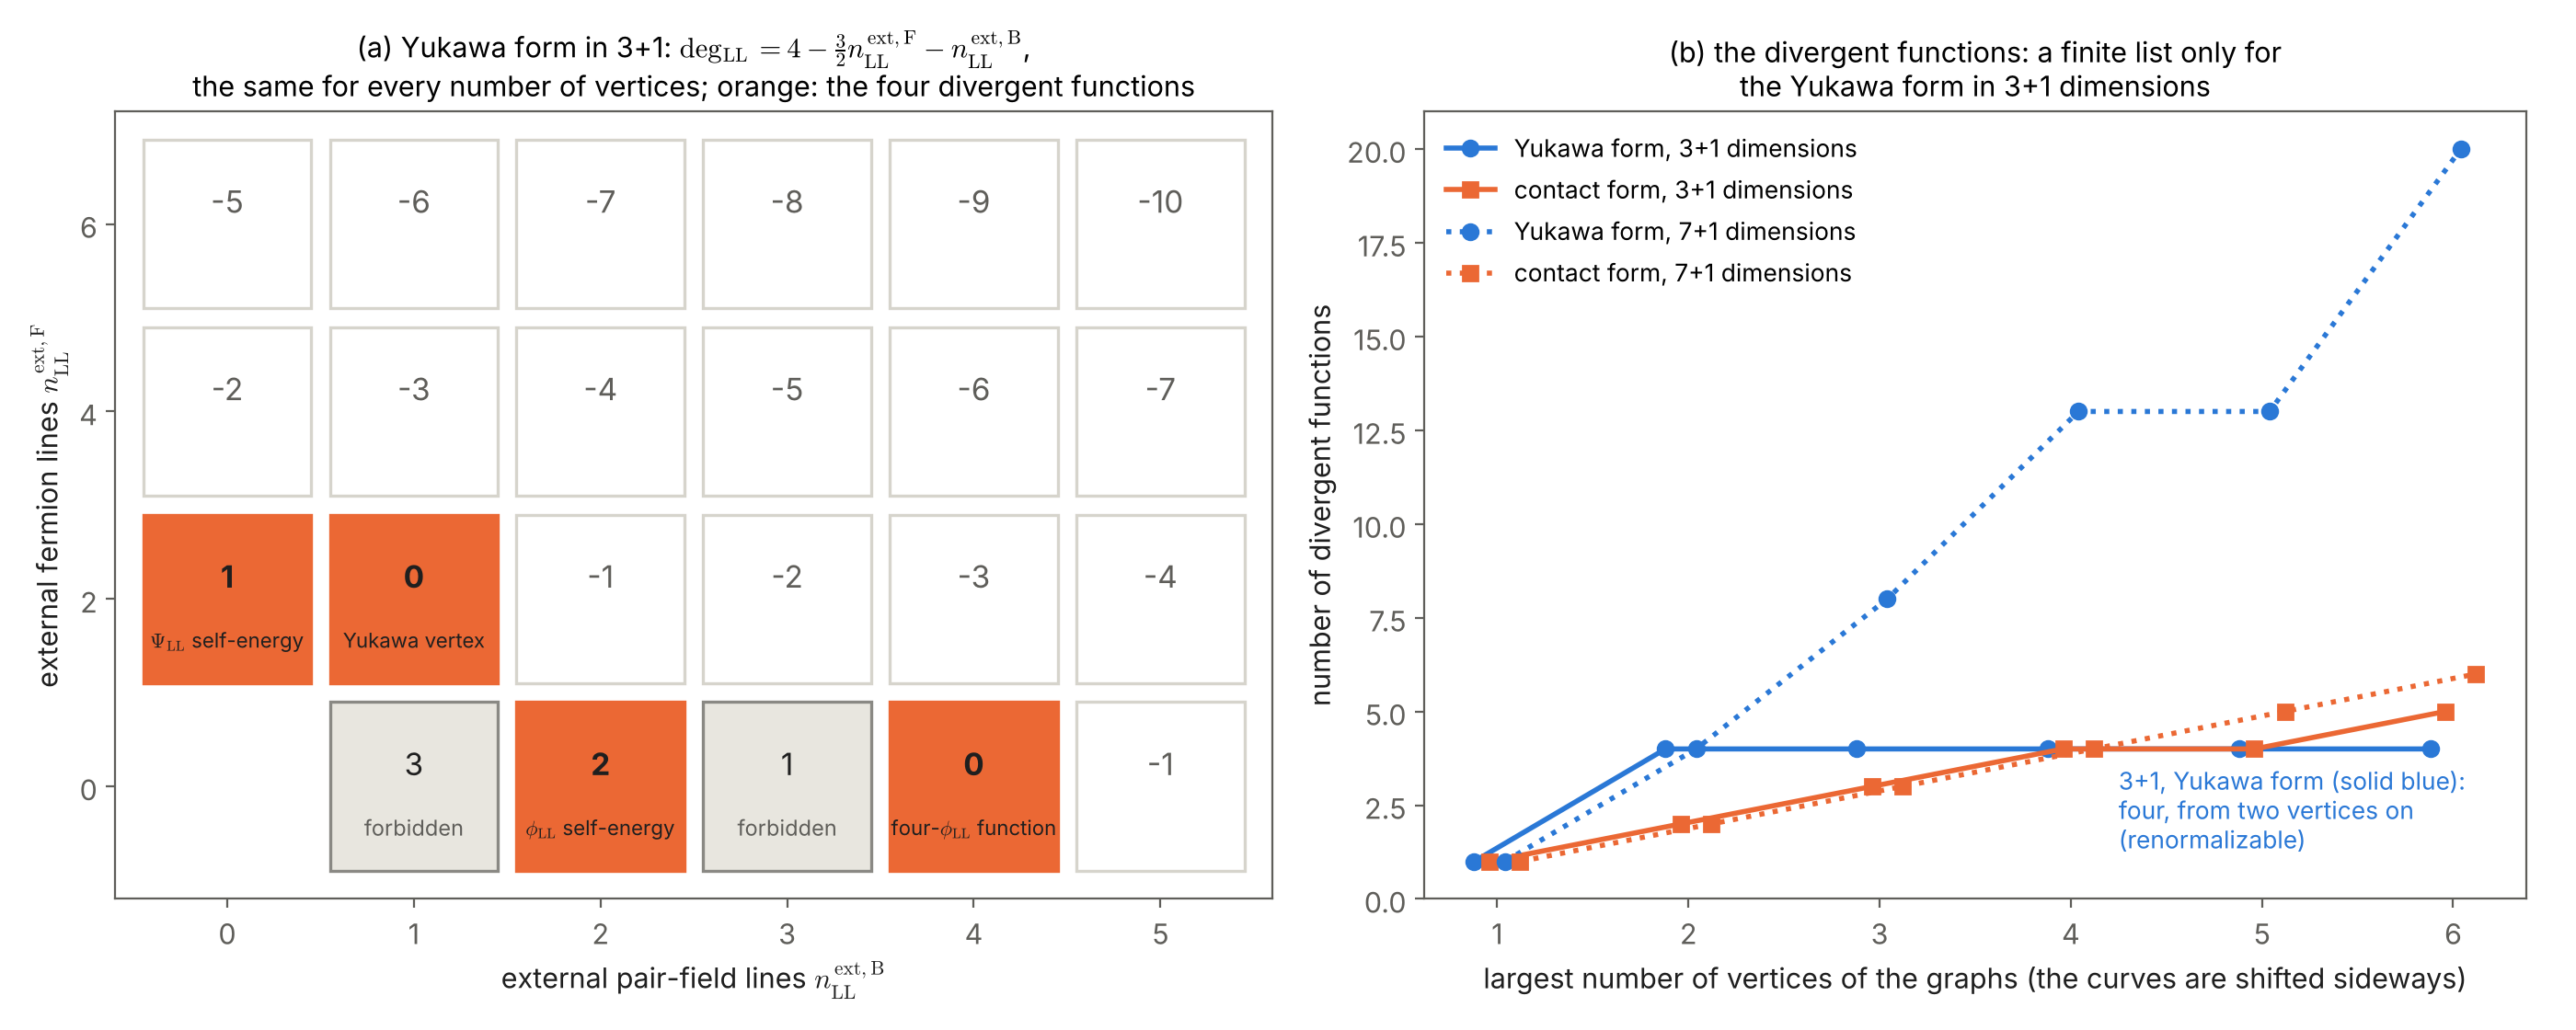
\includegraphics[width=1\textwidth,height=\textheight]{figures/fig_ex_r13_divergences.png}

\textbf{Figure 3.} The divergences, counted.

\begin{itemize}
\tightlist
\item
  \textbf{(a) The Yukawa form in \(3+1\) dimensions.} Each cell is one
  function, labelled by its numbers of external fermion lines (rows) and
  external pair-field lines (columns). The cell shows the superficial
  degree \(\deg_{\rm LL}\), which is the same at every order.

  \begin{itemize}
  \tightlist
  \item
    The four orange cells are the divergent functions of the table
    above.
  \item
    The two grey cells (marked ``forbidden'') have \(\deg_{\rm LL}\ge0\)
    but vanish by fermion-number conservation.
  \item
    Every white cell is convergent.
  \item
    The empty corner is the vacuum energy.
  \end{itemize}
\item
  \textbf{(b) The number of divergent functions, against the largest
  number of vertices of the graphs.} The four curves are shifted
  sideways by small amounts so that equal values stay visible.

  \begin{itemize}
  \tightlist
  \item
    Only for the Yukawa form in \(3+1\) dimensions (solid blue) does the
    number stop growing: four, from two vertices on.
  \item
    For the contact form, and for both forms in \(7+1\) dimensions, it
    grows with the order.
  \end{itemize}
\end{itemize}

Data: \texttt{explanations/data/ex\_r13\_power\_counting.csv} and
\texttt{ex\_r13\_divergent\_counts.csv}; check Z-7; drawn by
\texttt{explanations/code/make\_r13\_figures.py}.

The counts behind panel (b), from the data file
\texttt{ex\_r13\_divergent\_counts.csv}. The columns are the largest
number of vertices of the graphs:

\begin{longtable}[]{@{}lllllll@{}}
\toprule\noalign{}
form, dimensions & 1 & 2 & 3 & 4 & 5 & 6 \\
\midrule\noalign{}
\endhead
\bottomrule\noalign{}
\endlastfoot
Yukawa form, 3+1 & 1 & 4 & 4 & 4 & 4 & 4 \\
contact form, 3+1 & 1 & 2 & 3 & 4 & 4 & 5 \\
Yukawa form, 7+1 & 1 & 4 & 8 & 13 & 13 & 20 \\
contact form, 7+1 & 1 & 2 & 3 & 4 & 5 & 6 \\
\end{longtable}

\hypertarget{an-explicit-example-the-one-loop-bubble}{%
\subsection{5.4 An explicit example: the one-loop
bubble}\label{an-explicit-example-the-one-loop-bubble}}

The simplest divergent function is the self-energy of the pair field at
one loop: a fermion loop with two Yukawa vertices. After the traces over
the Dirac and isospin indices it is a constant times the Euclidean
\textbf{bubble}. The loop momentum \(k^{\rm E}_{\rm LL}\) and the
external momentum \(p^{\rm E}_{\rm LL}\) are continued to four Euclidean
dimensions, and a cutoff \(\Lambda_{\rm LL}\) is put on the length of
the loop momentum:
\[I^{\rm bub}_{\rm LL}(p^{\rm E}_{\rm LL})=\int_{\lvert k^{\rm E}_{\rm LL}\rvert<\Lambda_{\rm LL}}\frac{d^4k^{\rm E}_{\rm LL}}{(2\pi)^4}\;\frac{k^{\rm E}_{\rm LL}\cdot(k^{\rm E}_{\rm LL}+p^{\rm E}_{\rm LL})+m_{\rm LL}^2}{\big[(k^{\rm E}_{\rm LL})^2+m_{\rm LL}^2\big]\big[(k^{\rm E}_{\rm LL}+p^{\rm E}_{\rm LL})^2+m_{\rm LL}^2\big]} . \tag{5.4}\]
The constant factor depends on \(g^{\rm Y}_{\rm LL}\) and on the
normalization of the pair matrices, but not on the cutoff, and is
omitted. Power counting gives \(\deg_{\rm LL}=4-2=2\) (two fermion
propagators).

\textbf{How the program computes it} (check Z-8). It takes
\(\lvert p^{\rm E}_{\rm LL}\rvert=1\) and \(m_{\rm LL}=0.5\), in an
arbitrary unit of momentum, and cutoffs from 4 to 2048 (doubling each
time). The integral is computed in two steps:

\begin{itemize}
\tightlist
\item
  the average of the integrand over the directions of
  \(k^{\rm E}_{\rm LL}\), by a 48-point Gauss-Legendre rule in the angle
  between \(k^{\rm E}_{\rm LL}\) and \(p^{\rm E}_{\rm LL}\), with the
  weight of the four-dimensional sphere;
\item
  the integral over the length of \(k^{\rm E}_{\rm LL}\), with the
  measure
  \(\lvert k^{\rm E}_{\rm LL}\rvert^3d\lvert k^{\rm E}_{\rm LL}\rvert/(8\pi^2)\),
  by the same 48-point rule on the panels between the points
  \(0,\ 0.25,\ 0.375,\ 0.5625,\dots\) (each point 1.5 times the previous
  one), the last panel ending at \(\Lambda_{\rm LL}\).
\end{itemize}

The results:

\begin{itemize}
\tightlist
\item
  \textbf{The quadratic divergence is a constant.} At zero external
  momentum the integrand is \(1/[(k^{\rm E}_{\rm LL})^2+m_{\rm LL}^2]\),
  and
  \[I^{\rm bub}_{\rm LL}(0)=\frac1{16\pi^2}\Big[\Lambda_{\rm LL}^2-m_{\rm LL}^2\ln\Big(1+\frac{\Lambda_{\rm LL}^2}{m_{\rm LL}^2}\Big)\Big],\]
  which grows like \(\Lambda_{\rm LL}^2\). The program confirms the
  closed form and the growth. A constant is absorbed by the \textbf{mass
  counterterm} of \(\phi_{\rm LL}\).
\item
  \textbf{The logarithmic divergence is proportional to
  \((p^{\rm E}_{\rm LL})^2\).} The derivative of the momentum-dependent
  part,
  \(I^{\rm bub}_{\rm LL}(p^{\rm E}_{\rm LL})-I^{\rm bub}_{\rm LL}(0)\),
  with respect to \(\ln\Lambda_{\rm LL}\) is
  \(\Lambda_{\rm LL}^4/(8\pi^2)\) times the difference of the
  directional averages of the integrand on the sphere
  \(\lvert k^{\rm E}_{\rm LL}\rvert=\Lambda_{\rm LL}\). For large loop
  momenta the difference is
  \(-(p^{\rm E}_{\rm LL})^2/[2(k^{\rm E}_{\rm LL})^4]\). (Expand the
  integrand to second order in \(p^{\rm E}_{\rm LL}\); the average of
  \((k^{\rm E}_{\rm LL}\cdot p^{\rm E}_{\rm LL})^2\) over the directions
  of four-dimensional space is
  \(\tfrac14(k^{\rm E}_{\rm LL})^2(p^{\rm E}_{\rm LL})^2\).) So the
  derivative tends to \(-(p^{\rm E}_{\rm LL})^2/(16\pi^2)\). A term
  proportional to \((p^{\rm E}_{\rm LL})^2\) is absorbed by the
  \textbf{wave-function counterterm}.
\item
  \textbf{Nothing else diverges.} The directional average of the
  integrand, expanded in \(p^{\rm E}_{\rm LL}\), has:

  \begin{itemize}
  \tightlist
  \item
    the coefficient
    \(-[(k^{\rm E}_{\rm LL})^2+2m_{\rm LL}^2]/(2[(k^{\rm E}_{\rm LL})^2+m_{\rm LL}^2]^3)\)
    of \((p^{\rm E}_{\rm LL})^2\);
  \item
    the coefficient
    \(m_{\rm LL}^4/[(k^{\rm E}_{\rm LL})^2+m_{\rm LL}^2]^5\) of
    \((p^{\rm E}_{\rm LL})^4\) (checked numerically by the program);
  \item
    no odd powers, because the average depends only on
    \((p^{\rm E}_{\rm LL})^2\).
  \end{itemize}

  The \textbf{renormalized bubble} is the bubble minus the two
  counterterms,
  \[I^{\rm ren}_{\rm LL}(p^{\rm E}_{\rm LL})=I^{\rm bub}_{\rm LL}(p^{\rm E}_{\rm LL})-I^{\rm bub}_{\rm LL}(0)-(p^{\rm E}_{\rm LL})^2\,\frac{\partial I^{\rm bub}_{\rm LL}}{\partial(p^{\rm E}_{\rm LL})^2}\Big|_{p^{\rm E}_{\rm LL}=0}.\]
  Its directional average starts with the power
  \((p^{\rm E}_{\rm LL})^4\).

  \begin{itemize}
  \tightlist
  \item
    \textbf{What power counting guarantees.} Each power of
    \(p^{\rm E}_{\rm LL}\) costs one power of the loop momentum, so the
    term of order \((p^{\rm E}_{\rm LL})^4\) falls at least like
    \(\lvert k^{\rm E}_{\rm LL}\rvert^{-6}\). With the measure
    \(\lvert k^{\rm E}_{\rm LL}\rvert^3\) the radial integrand falls at
    least like \(\lvert k^{\rm E}_{\rm LL}\rvert^{-3}\), and the change
    of \(I^{\rm ren}_{\rm LL}\) per doubling of the cutoff falls at
    least like \(\Lambda_{\rm LL}^{-2}\): a factor 4 per doubling.
  \item
    \textbf{What the calculation shows.} The coefficient
    \(m_{\rm LL}^4/[(k^{\rm E}_{\rm LL})^2+m_{\rm LL}^2]^5\) falls like
    \(\lvert k^{\rm E}_{\rm LL}\rvert^{-10}\), because the leading terms
    cancel in the average over the directions. The radial integrand then
    falls like \(\lvert k^{\rm E}_{\rm LL}\rvert^{-7}\), and each
    doubling divides the change by about \(2^6=64\).
  \end{itemize}
\end{itemize}

The computed values (data file \texttt{ex\_r13\_bubble.csv}):

\begin{longtable}[]{@{}
  >{\raggedright\arraybackslash}p{(\columnwidth - 10\tabcolsep) * \real{0.0732}}
  >{\raggedright\arraybackslash}p{(\columnwidth - 10\tabcolsep) * \real{0.1707}}
  >{\raggedright\arraybackslash}p{(\columnwidth - 10\tabcolsep) * \real{0.1707}}
  >{\raggedright\arraybackslash}p{(\columnwidth - 10\tabcolsep) * \real{0.2195}}
  >{\raggedright\arraybackslash}p{(\columnwidth - 10\tabcolsep) * \real{0.1707}}
  >{\raggedright\arraybackslash}p{(\columnwidth - 10\tabcolsep) * \real{0.1951}}@{}}
\toprule\noalign{}
\begin{minipage}[b]{\linewidth}\raggedright
\(\Lambda_{\rm LL}\)
\end{minipage} & \begin{minipage}[b]{\linewidth}\raggedright
\(I^{\rm bub}_{\rm LL}(0)\) computed
\end{minipage} & \begin{minipage}[b]{\linewidth}\raggedright
\(I^{\rm bub}_{\rm LL}(0)\) closed form
\end{minipage} & \begin{minipage}[b]{\linewidth}\raggedright
\(d[I^{\rm bub}_{\rm LL}(p^{\rm E}_{\rm LL})-I^{\rm bub}_{\rm LL}(0)]/d\ln\Lambda_{\rm LL}\)
\end{minipage} & \begin{minipage}[b]{\linewidth}\raggedright
\(I^{\rm ren}_{\rm LL}\)
\end{minipage} & \begin{minipage}[b]{\linewidth}\raggedright
change of \(I^{\rm ren}_{\rm LL}\) from \(\Lambda_{\rm LL}/2\)
\end{minipage} \\
\midrule\noalign{}
\endhead
\bottomrule\noalign{}
\endlastfoot
4 & \(9.471253\times10^{-2}\) & \(9.471253\times10^{-2}\) &
\(-6.233478\times10^{-3}\) & \(1.560633\times10^{-3}\) & --- \\
8 & \(3.964998\times10^{-1}\) & \(3.964998\times10^{-1}\) &
\(-6.307835\times10^{-3}\) & \(1.560665\times10^{-3}\) &
\(3.208453\times10^{-8}\) \\
16 & \(1.610164\) & \(1.610164\) & \(-6.326390\times10^{-3}\) &
\(1.560666\times10^{-3}\) & \(4.968769\times10^{-10}\) \\
32 & \(6.471387\) & \(6.471387\) & \(-6.331028\times10^{-3}\) &
\(1.560666\times10^{-3}\) & \(7.745994\times10^{-12}\) \\
64 & \(2.592286\times10^{1}\) & \(2.592286\times10^{1}\) &
\(-6.332187\times10^{-3}\) & \(1.560666\times10^{-3}\) &
\(1.200301\times10^{-13}\) \\
128 & \(1.037353\times10^{2}\) & \(1.037353\times10^{2}\) &
\(-6.332477\times10^{-3}\) & \(1.560666\times10^{-3}\) &
\(6.415875\times10^{-15}\) \\
256 & \(4.149918\times10^{2}\) & \(4.149918\times10^{2}\) &
\(-6.332550\times10^{-3}\) & \(1.560666\times10^{-3}\) &
\(2.449018\times10^{-14}\) \\
512 & \(1.660024\times10^{3}\) & \(1.660024\times10^{3}\) &
\(-6.332568\times10^{-3}\) & \(1.560666\times10^{-3}\) &
\(1.993965\times10^{-13}\) \\
1024 & \(6.640161\times10^{3}\) & \(6.640161\times10^{3}\) &
\(-6.332572\times10^{-3}\) & \(1.560666\times10^{-3}\) &
\(3.827856\times10^{-13}\) \\
2048 & \(2.656071\times10^{4}\) & \(2.656071\times10^{4}\) &
\(-6.332574\times10^{-3}\) & \(1.560666\times10^{-3}\) &
\(1.132425\times10^{-12}\) \\
\end{longtable}

Read the table column by column:

\begin{itemize}
\tightlist
\item
  \textbf{\(I^{\rm bub}_{\rm LL}(0)\)} agrees with its closed form and
  grows by a factor of 4 per doubling of the cutoff:
  \(\Lambda_{\rm LL}^2\).
\item
  \textbf{The slope} tends to \(-1/(16\pi^2)\) for
  \(\lvert p^{\rm E}_{\rm LL}\rvert=1\): a logarithm. The program
  \texttt{superloop} found the same slope independently, with a
  different quadrature, \(-6.332440\times10^{-3}\) against
  \(-6.332574\times10^{-3}\) (ratio \(0.99998\), check R-4 in Section
  7.3).
\item
  \textbf{The renormalized bubble} settles at a constant. Its change per
  doubling falls by a factor of about 64 until it reaches the rounding
  errors of double precision (from \(\Lambda_{\rm LL}=128\) on).
\end{itemize}

\textbf{After the two counterterms nothing depends on the cutoff.} This
is renormalization at work, in the simplest case.

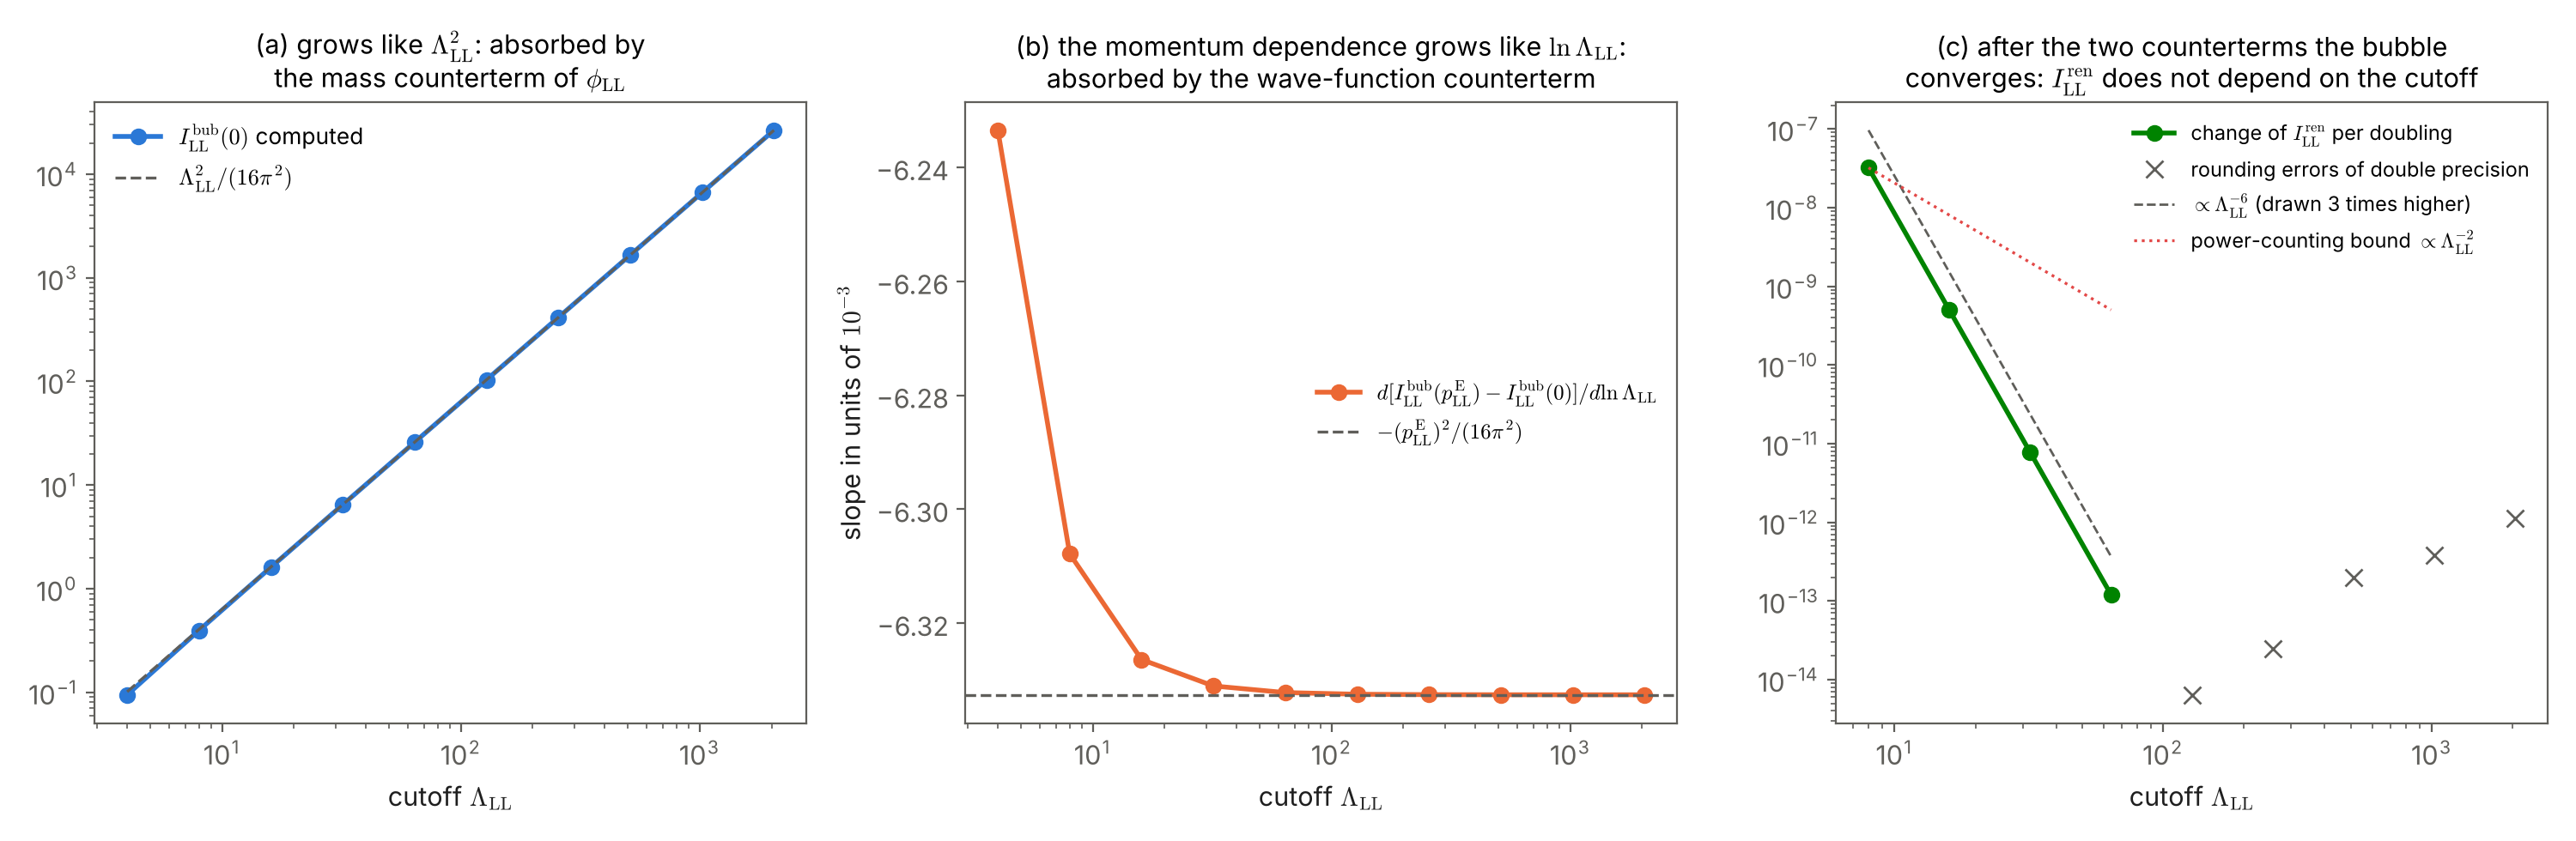
\includegraphics[width=1\textwidth,height=\textheight]{figures/fig_ex_r13_bubble.png}

\textbf{Figure 4.} The one-loop bubble (5.4) at
\(\lvert p^{\rm E}_{\rm LL}\rvert=1\), \(m_{\rm LL}=0.5\), against the
cutoff.

\begin{itemize}
\tightlist
\item
  \textbf{(a)} \(I^{\rm bub}_{\rm LL}(0)\) follows
  \(\Lambda_{\rm LL}^2/(16\pi^2)\) (dashed): a quadratic divergence,
  absorbed by the mass counterterm.
\item
  \textbf{(b)} The cutoff derivative of
  \(I^{\rm bub}_{\rm LL}(p^{\rm E}_{\rm LL})-I^{\rm bub}_{\rm LL}(0)\)
  tends to \(-(p^{\rm E}_{\rm LL})^2/(16\pi^2)\) (dashed): a logarithmic
  divergence, absorbed by the wave-function counterterm.
\item
  \textbf{(c)} The change of the renormalized bubble per doubling of the
  cutoff (green) falls like \(\Lambda_{\rm LL}^{-6}\). The dashed line
  of that slope is drawn three times higher so as not to hide the data.
  The fall is faster than the power-counting bound
  \(\Lambda_{\rm LL}^{-2}\) (red, dotted). From \(\Lambda_{\rm LL}=128\)
  on, the changes are rounding errors of double precision (crosses).
\end{itemize}

Data: \texttt{explanations/data/ex\_r13\_bubble.csv}; check Z-8; drawn
by \texttt{explanations/code/make\_r13\_figures.py}.

\hypertarget{the-contact-form-is-not-renormalizable}{%
\subsection{5.5 The contact form is not
renormalizable}\label{the-contact-form-is-not-renormalizable}}

The contact coupling has the mass dimension \(-2\) in \(3+1\)
dimensions. By Eq. (5.3), the degree of divergence grows by 2 with every
contact vertex. The four-fermion function, the six-fermion function and
so on all diverge at high enough order, and infinitely many counterterms
would be needed (Figure 3(b)).

The superfluid calculation shows the same thing directly.

\begin{itemize}
\tightlist
\item
  \textbf{The gap equation.} For the unitary scalar superfluid with the
  gap \(\Delta_{\rm LL}\), the gap equation of the contact form is
  \[\frac1{G_{\rm LL}}=\int_{q_{\rm LL}<\Lambda_{\rm LL}}\frac{d^3q_{\rm LL}}{(2\pi)^3}\Big(\frac1{E^+_{\rm LL}}+\frac1{E^-_{\rm LL}}\Big),\qquad E^\pm_{\rm LL}=\big[(\varepsilon_{\rm LL}\pm\mu_{\rm LL})^2+\Delta_{\rm LL}^2\big]^{1/2},\quad\varepsilon_{\rm LL}=(q_{\rm LL}^2+m_{\rm LL}^2)^{1/2},\]
  with the momentum \(\vec q_{\rm LL}\) of a spinor charge and its
  length \(q_{\rm LL}\).
\item
  \textbf{Its large-momentum part.} For \(q_{\rm LL}\) much larger than
  \(\mu_{\rm LL}\), \(m_{\rm LL}\) and \(\Delta_{\rm LL}\), the bracket
  is \(2/q_{\rm LL}\). Since
  \(d^3q_{\rm LL}/(2\pi)^3=q_{\rm LL}^2\,dq_{\rm LL}/(2\pi^2)\) after
  the angular integration, the integral grows like
  \(\int^{\Lambda_{\rm LL}}q_{\rm LL}\,dq_{\rm LL}/\pi^2=\Lambda_{\rm LL}^2/(2\pi^2)\).
  The remaining terms grow at most like \(\ln\Lambda_{\rm LL}\).
\item
  \textbf{The consequence.} At a fixed physical gap the bare coupling
  must fall like the inverse square of the cutoff:
  \(G_{\rm LL}\Lambda_{\rm LL}^2/(2\pi^2)\to1\).
\item
  \textbf{The computed value.} The program \texttt{superloop} solves the
  gap equation at \(\Delta_{\rm LL}=0.05\), \(\mu_{\rm LL}=0.5\),
  \(m_{\rm LL}=0.2\). It finds
  \(G_{\rm LL}\Lambda_{\rm LL}^2/(2\pi^2)=\)\(0.99981\) at
  \(\Lambda_{\rm LL}=128\) (check R-3 in Section 7.3).
\end{itemize}

The cutoff cannot be removed with finitely many logarithmic
counterterms. Like the model of Nambu and Jona-Lasinio, the contact form
is an effective theory, valid below the cutoff. The Yukawa form (4.2) is
its renormalizable completion, with
\(G_{\rm LL}=4(g^{\rm Y}_{\rm LL})^2/(m^\phi_{\rm LL})^2\).

\hypertarget{why-not-on-the-eight-dimensional-manifolds}{%
\subsection{5.6 Why not on the eight-dimensional
manifolds}\label{why-not-on-the-eight-dimensional-manifolds}}

On the \(7+1\) manifold \(\mathbb R^{1,7}_{\rm LL}\) the fields depend
on seven space coordinates: \(D=7\). On the \(4+4\) manifold (the split
octonions, with four time-like and four space-like directions) the
propagators have a different singularity structure, but the mass
dimensions, and with them the power counting, depend only on the total
number of coordinates, 8, as for \(D=7\). The table of Section 5.1
gives:

\begin{itemize}
\tightlist
\item
  \([g^{\rm Y}_{\rm LL}]=-2\),
  \([\lambda^{(1)}_{\rm LL}]=[\lambda^{(2)}_{\rm LL}]=-4\) and
  \([G_{\rm LL}]=-6\): every coupling has a negative dimension;
\item
  by Eq. (5.2),
  \(\deg_{\rm LL}=8-\tfrac72n^{\rm ext,F}_{\rm LL}-3n^{\rm ext,B}_{\rm LL}+4(\tfrac12n^{\rm v,Y}_{\rm LL}+n^{\rm v,4}_{\rm LL})\),
  which grows by 2 with every Yukawa vertex and by 4 with every quartic
  vertex.
\end{itemize}

The number of divergent functions of the Yukawa form grows without
bound: 1, 4, 8, 13, 13, 20 for graphs with at most 1 to 6 vertices
(Figure 3(b) and the table of counts). \textbf{Neither form is
renormalizable in eight dimensions.} This is why the statement says ``in
\(3+1\) dimensions''.

\hypertarget{non-associativity-changes-nothing-and-what-is-and-is-not-proved}{%
\subsection{5.7 Non-associativity changes nothing, and what is and is
not
proved}\label{non-associativity-changes-nothing-and-what-is-and-is-not-proved}}

\textbf{Non-associativity.} A Lagrangian is built from fields on which
the symmetries act linearly, and a linear action of the super-loop
generates a Lie group. The counterterms that the loop allows are
therefore those that its Lie closure allows. Check R-6 of the program
\texttt{superloop} makes this precise in the simplest case. It compares
two spaces of quadratic forms on \(\mathbb B_{\rm LL}\):

\begin{itemize}
\tightlist
\item
  the forms invariant under the 14 left multiplications by the imaginary
  bi-octonions;
\item
  the forms invariant under the 56-dimensional Lie algebra that these
  multiplications generate.
\end{itemize}

The two spaces are the same two-dimensional space, spanned by the real
and imaginary parts of \(N_{\rm LL}\). Power counting, and hence
renormalizability, is unchanged by the non-associativity of the
super-loop.

\textbf{What is proved here:}

\begin{itemize}
\tightlist
\item
  the couplings of the Yukawa form are dimensionless in \(3+1\)
  dimensions (Section 5.1);
\item
  exactly four functions diverge superficially, at every order: by Eq.
  (5.2), and checked for all classes of graphs with up to six vertices
  (Sections 5.2 and 5.3);
\item
  the Lagrangian contains a term to absorb each of them (Section 5.3);
\item
  at one loop the two counterterms make the self-energy of the pair
  field finite (Section 5.4).
\end{itemize}

\textbf{What the standard theorem adds.} The renormalization theorem of
Bogoliubov and Parasiuk, Hepp, and Zimmermann then guarantees that the
divergences can be removed to all orders by counterterms of these forms.
The theorem applies to a theory with two properties:

\begin{itemize}
\tightlist
\item
  every coupling has a mass dimension of zero or more;
\item
  the Lagrangian contains every term of dimension at most 4 that its
  symmetries allow.
\end{itemize}

The symmetries used (Lorentz, isospin, fermion number, parity) act
linearly on the fields. The subtraction of Taylor terms in the external
momenta, carried out directly in four dimensions, respects all of them,
and all the fields are massive.

\textbf{What was not computed:} the explicit renormalization beyond one
loop, and the running of the couplings.

\hypertarget{the-answers-to-the-test-in-one-table}{%
\section{6. The answers to the test, in one
table}\label{the-answers-to-the-test-in-one-table}}

\begin{longtable}[]{@{}
  >{\raggedright\arraybackslash}p{(\columnwidth - 4\tabcolsep) * \real{0.2000}}
  >{\raggedright\arraybackslash}p{(\columnwidth - 4\tabcolsep) * \real{0.6250}}
  >{\raggedright\arraybackslash}p{(\columnwidth - 4\tabcolsep) * \real{0.1750}}@{}}
\toprule\noalign{}
\begin{minipage}[b]{\linewidth}\raggedright
question
\end{minipage} & \begin{minipage}[b]{\linewidth}\raggedright
answer
\end{minipage} & \begin{minipage}[b]{\linewidth}\raggedright
where computed
\end{minipage} \\
\midrule\noalign{}
\endhead
\bottomrule\noalign{}
\endlastfoot
What is the \(3+1\) manifold? & \(\mathbb R^{1,3}_{\rm LL}\), the
Hermitian bi-quaternions
\(x^0_{\rm LL}\mathbf e_0+i\sum_jx^j_{\rm LL}\mathbf e_j\), with the
matrix \(M_{\rm LL}(\mathbf x)=\sum_px^p_{\rm LL}\sigma^{\rm LL}_p\) &
Section 2; Z-1 \\
Its coordinates? &
\(x^0_{\rm LL}=\tfrac12\mathrm{tr}\,M_{\rm LL}(\mathbf x)\) (time) and
\(x^j_{\rm LL}=\tfrac12\mathrm{tr}(\sigma^{\rm LL}_jM_{\rm LL}(\mathbf x))\)
(space), along \(\mathbf e_0\), \(i\mathbf e_1\), \(i\mathbf e_2\),
\(i\mathbf e_3\) & Figure 1; Z-1 \\
Its metric? &
\(N_{\rm LL}=\det M_{\rm LL}(\mathbf x)=(x^0_{\rm LL})^2-\sum_j(x^j_{\rm LL})^2\),
signature (1,3): Minkowski space & Z-2 \\
Its symmetry, and the super-loop? &
\(\mathbf x\mapsto\mathbf g\mathbf x\mathbf g^\dagger\) for the unit
bi-quaternions \(\mathbf g\) of the super-loop: all proper orthochronous
Lorentz transformations, each from exactly \(\pm\mathbf g\) (double
cover \(SL(2,\mathbb C)\)), generated by \(J^j_{\rm LL}\) and
\(K^j_{\rm LL}\) & Section 3; Z-3, Z-4; Figure 2 \\
Examples? & the sample point; a boost; a rotation; the rotation by
\(2\pi\); a spinor and its null point; the spinor charges as spinors &
Z-5 \\
The theory on it? & the Dirac isodoublet \(\Psi_{\rm LL}\) of the spinor
charges and the pair field \(\phi_{\rm LL}\), Lagrangian (4.2) & Section
4 \\
Why renormalizable in \(3+1\)? & dimensionless couplings;
\(\deg_{\rm LL}=4-\tfrac32n^{\rm ext,F}_{\rm LL}-n^{\rm ext,B}_{\rm LL}\)
at every order; four divergent functions, each absorbed by a term of Eq.
(4.2) & Z-6, Z-7; Figure 3 \\
An explicit check? & the one-loop bubble: the \(\Lambda_{\rm LL}^2\) and
\(\ln\Lambda_{\rm LL}\) divergences are absorbed by two counterterms,
and the remainder converges & Z-8; Figure 4 \\
Why not in eight dimensions? & all couplings have negative mass
dimensions; the number of divergent functions grows without bound & Z-6,
Z-7 \\
\end{longtable}

\hypertarget{provenance-programs-commands-reports-data-figures}{%
\section{7. Provenance: programs, commands, reports, data,
figures}\label{provenance-programs-commands-reports-data-figures}}

\hypertarget{how-to-reproduce-everything}{%
\subsection{7.1 How to reproduce
everything}\label{how-to-reproduce-everything}}

From the folder Revision\_SuperLoop of the repository:

\begin{verbatim}
# 1. the examples and checks of this document (explanations/data/ex_r13_*), checks Z-1 to Z-8
(cd explanations && cargo run --release --manifest-path code/r13-rs/Cargo.toml)
# 2. its four figures (explanations/figures/fig_ex_r13_*.pdf and .png)
python3 explanations/code/make_r13_figures.py
# 3. the checks R-1 to R-6 and N-1 to N-9 of the program superloop quoted here
cargo run --release --manifest-path code/superloop-rs/Cargo.toml -- renorm
cargo run --release --manifest-path code/superloop-rs/Cargo.toml -- manifolds
# 4. everything of the folder, all checks and all documents, with one verdict ("ALL PASS")
bash code/scripts/check_all.sh
\end{verbatim}

Requirements:

\begin{itemize}
\tightlist
\item
  a Rust toolchain for the edition 2021;
\item
  Python 3 with NumPy and Matplotlib;
\item
  for the documents: pandoc (version 2.11 or later), XeLaTeX and
  latexmk, the DejaVu fonts and the Latin Modern Math font.
\end{itemize}

The Rust programs use the library crate \texttt{code/spacetimes-rs} of
the repository (complex numbers and matrices, Gauss-Legendre rules, the
writer of data files); no other crate is used.

\hypertarget{the-program-of-this-document}{%
\subsection{7.2 The program of this
document}\label{the-program-of-this-document}}

\texttt{explanations/code/r13-rs/src/main.rs} (923 lines of commented
Rust, binary \texttt{r13\_yukawa}) computes every number and curve of
this document and checks:

\begin{itemize}
\tightlist
\item
  \textbf{Z-1} the coordinates and the matrix map (2.2);
\item
  \textbf{Z-2} the signature;
\item
  \textbf{Z-3} the Lorentz group (3.1);
\item
  \textbf{Z-4} the six generators and the relations (3.2);
\item
  \textbf{Z-5} the worked examples, the spinors and the spinor charges;
\item
  \textbf{Z-6} the mass dimensions;
\item
  \textbf{Z-7} the power counting (5.1) to (5.3) and the list of
  divergent functions;
\item
  \textbf{Z-8} the bubble (5.4) and its renormalization.
\end{itemize}

The arithmetic is double precision; the power counting uses exact
integers. Equalities are tested with the absolute tolerance \(10^{-12}\)
unless the statement of the check names another tolerance; Z-3, Z-4, Z-5
and Z-8 name theirs. The random numbers come from a fixed seed, so every
run gives the same output.

The report, verbatim (\texttt{explanations/data/ex\_r13\_checks.txt}).
It writes the symbols with the plain-text names of the table of Section
9, for example:

\begin{itemize}
\tightlist
\item
  \texttt{x\_LL\^{}p}, \texttt{N\_LL}, \texttt{M\_LL}, \texttt{Lmat},
  \texttt{V\_LL} for \(x^p_{\rm LL}\), \(N_{\rm LL}\), \(M_{\rm LL}\),
  \(\mathsf L_{\rm LL}\), \(\mathcal V_{\rm LL}\);
\item
  \texttt{gL}, \texttt{hL}, \texttt{gLbar}, \texttt{uL}, \texttt{bS} for
  \(\mathbf g\), \(\mathbf h\), \(\bar{\mathbf g}\), \(\mathbf u\),
  \(\mathbf b\);
\item
  \texttt{sigma\_j}, \texttt{eps2}, \texttt{eps3}, \texttt{chi},
  \texttt{psi\textquotesingle{}\_LL}, \texttt{theta} for
  \(\sigma^{\rm LL}_j\), \(\mathsf E_{\rm LL}\),
  \(\epsilon^{\rm LL}_{jj'j''}\), \(\chi_{\rm LL}\), \(\psi'_{\rm LL}\),
  \(\theta_{\rm LL}\);
\item
  \texttt{phi}, \texttt{G}, \texttt{g\_Y}, \texttt{lam4},
  \texttt{m\_phi}, \texttt{m} for \(\phi_{\rm LL}\), \(G_{\rm LL}\),
  \(g^{\rm Y}_{\rm LL}\), the quartic couplings, \(m^\phi_{\rm LL}\),
  \(m_{\rm LL}\);
\item
  \texttt{kE}, \texttt{pE}, \texttt{Lambda}, \texttt{Ibub},
  \texttt{Iren} for \(k^{\rm E}_{\rm LL}\), \(p^{\rm E}_{\rm LL}\),
  \(\Lambda_{\rm LL}\), \(I^{\rm bub}_{\rm LL}\),
  \(I^{\rm ren}_{\rm LL}\).
\end{itemize}

\begin{verbatim}
Revision_SuperLoop, folder explanations, program `r13_yukawa`: the 3+1 manifold R^(1,3)_LL of the super-loop and the renormalizability of the Yukawa form on it
8 of 8 checks passed

[PASS] Z-1  the coordinates of R^(1,3)_LL: the Hermitian bi-quaternion x = x_LL^0 e0 + i (x_LL^1 e1 + x_LL^2 e2 + x_LL^3 e3) with real coordinates has the matrix M_LL(x) = x_LL^0 sigma_0 + x_LL^1 sigma_1 + x_LL^2 sigma_2 + x_LL^3 sigma_3 (M_LL(e0) = sigma_0, M_LL(i e_j) = sigma_j), which is Hermitian; det M_LL(x) = N_LL(x) = (x_LL^0)^2 - (x_LL^1)^2 - (x_LL^2)^2 - (x_LL^3)^2; the coordinates are recovered as x_LL^0 = tr M_LL(x)/2 and x_LL^j = tr(sigma_j M_LL(x))/2  -- the four basis elements and 200 random points
[PASS] Z-2  R^(1,3)_LL is Minkowski space: the symmetric matrix of the quadratic form N_LL = det M_LL(x) in the coordinates x_LL^0..x_LL^3 (by polarization) is diag(1, -1, -1, -1): signature (1 positive, 3 negative)  -- matrix diag(1.000000, -1.000000, -1.000000, -1.000000)
[PASS] Z-3  the Lorentz group of R^(1,3)_LL: for 200 random unit bi-quaternions gL (random matrices M_LL(gL) in SL(2,C): four entries with real and imaginary parts uniform in [-1, 1), accepted if the modulus of the determinant exceeds 0.1, divided by a square root of the determinant; tolerances 1e-10 for the 2 x 2 matrices, 1e-9 for Lmat and the coordinates, 1e-12 for Lmat(gL) against Lmat(-gL)), M_LL(x) -> M_LL(gL) M_LL(x) M_LL(gL)^dag keeps the matrix Hermitian and keeps N_LL(x); its matrix Lmat in the coordinates satisfies Lmat^T diag(1,-1,-1,-1) Lmat = diag(1,-1,-1,-1), det Lmat = 1 and Lmat[0][0] >= 1 (a proper orthochronous Lorentz transformation); gL and -gL give the same Lmat (SL(2,C) is the double cover), and Lmat(gL hL) = Lmat(gL) Lmat(hL) (a group homomorphism)  -- largest change of N_LL: 6.3e-14
[PASS] Z-4  the six generators: the rotation generators J_LL^j = e_j/2 and the boost generators K_LL^j = i e_j/2 of the super-loop have M_LL(J_LL^j) = -i sigma_j/2 and M_LL(K_LL^j) = sigma_j/2; their action M_LL(x) -> M_LL(uL) M_LL(x) + M_LL(x) M_LL(uL)^dag on R^(1,3)_LL gives six real 4 x 4 matrices V_LL(J_LL^j), V_LL(K_LL^j) (equal, within 1e-8, to the derivatives at theta = 0 of Lmat of the finite rotations exp(-i theta sigma_j/2) and boosts exp(theta sigma_j/2), computed by central differences with the step 1e-5), each preserving the metric (V_LL(uL)^T diag(1,-1,-1,-1) + diag(1,-1,-1,-1) V_LL(uL) = 0), linearly independent (the Gram matrix of their 16 entries has rank 6 in a Gaussian elimination with the pivot threshold 1e-9), with the relations of so(3,1): [V_LL(J_LL^j), V_LL(J_LL^j')] = sum_j'' eps3_jj'j'' V_LL(J_LL^j''), [V_LL(J_LL^j), V_LL(K_LL^j')] = sum_j'' eps3_jj'j'' V_LL(K_LL^j''), [V_LL(K_LL^j), V_LL(K_LL^j')] = -sum_j'' eps3_jj'j'' V_LL(J_LL^j'') (two boosts close into a rotation with the minus sign that distinguishes the Lorentz algebra from so(4))  -- rank 6, 27 commutation relations
[PASS] Z-5  worked examples on R^(1,3)_LL: the sample point (2, 1.2, 1.5, 1.0) has M_LL(x) = [[3, 1.2 - 1.5 i], [1.2 + 1.5 i, 1]] and N_LL = -0.69 (spacelike); the boost along x_LL^1 with the rapidity 0.8 takes (1, 0, 0, 0) to (cosh 0.8, sinh 0.8, 0, 0); the rotation about x_LL^3 by pi/3 takes (0, 1, 0, 0) to (0, 1/2, sqrt3/2, 0); the rotation by 2 pi has M_LL(gL) = -sigma_0 and Lmat = identity; a two-component spinor chi gives the null point with M_LL(x) = chi chi^dag (chi = (1, 0): (1/2, 0, 0, 1/2)), and the boost of chi along x_LL^3 with the rapidity 0.8 moves it along the light cone to exp(0.8) (1/2, 0, 0, 1/2); chi chi^dag is a future null point for 200 random chi; the Lorentz transformation gL acts on each column of the Weyl isodoublet psi'_LL = eps2^-1 M_LL(bS)^T of a spinor charge (bS -> bS gLbar) as chi -> M_LL(gL) chi, because eps2^-1 M_LL(gLbar)^T eps2 = M_LL(gL) (200 random gL as in Z-3, tolerance 1e-10)  -- sample point: N_LL = -0.690000; boost: (1.337435, 0.888106, 0, 0); rotation: (0, 0.500000, 0.866025, 0); null points checked: 200; columns checked: 200
[PASS] Z-6  mass dimensions in D + 1 space-time dimensions (every term of the Lagrangian density has the dimension D + 1): [Psi_LL] = D/2, [phi] = (D-1)/2, the contact coupling [G] = 1 - D, the Yukawa coupling [g_Y] = (3-D)/2, the quartic couplings [lam4] = 3 - D; for D = 3 (the manifold R^(1,3)_LL): 3/2, 1, -2, 0, 0 -- the Yukawa form has only couplings of dimension 0 and is renormalizable by power counting, the contact form is not; for D = 7 (R^(1,7)_LL, and the 4+4 manifold, where power counting sees the total dimension 8): 7/2, 3, -6, -2, -4 -- every coupling has a negative dimension; below the mass m_phi of the pair field its exchange gives the contact coupling G = 4 g_Y^2/m_phi^2, consistent with [G] = 2[g_Y] - 2  -- D = 3: 3/2, 1, -2, 0, 0; D = 7: 7/2, 3, -6, -2, -4
[PASS] Z-7  power counting (all classes of graphs with 1 to 6 vertices and at least one loop; a class is a set of numbers next_F, next_B, nvert_Y, nvert_4 for which the line ends at the vertices pair into internal lines, and deg depends only on the class; topological count nloop = nint_F + nint_B - nvert + 1, deg = (D+1) nloop - nint_F - 2 nint_B, compared with the formulas deg = (D+1) - D next_F/2 - (D-1) next_B/2 + (D-3)(nvert_Y/2 + nvert_4) of the Yukawa form and deg = (D+1) - D next_F/2 + (D-1) nvert of the contact form): in 3+1 dimensions the Yukawa form has, for the graphs with at most nvert vertices and every nvert from 2 to 6, exactly four divergent functions that conserve the fermion number (the pair-field self-energy, deg 2; the fermion self-energy, deg 1; the Yukawa vertex, deg 0; the four-point function of the pair field, deg 0) -- each has a term of the Lagrangian density to absorb it; the functions with one or three pair-field lines and no fermion lines (deg 3 and 1) vanish by fermion-number conservation; the number of divergent functions of the contact form grows with the number of vertices, and so does that of both forms for D = 7  -- 408 graph classes compared; Yukawa form, D = 3, divergent and allowed: (next_F, next_B) = (0, 2) deg 2, (next_F, next_B) = (0, 4) deg 0, (next_F, next_B) = (2, 0) deg 1, (next_F, next_B) = (2, 1) deg 0
[PASS] Z-8  the one-loop bubble of the Yukawa form, Ibub(pE) = int_(|kE| < Lambda) d^4kE/(2 pi)^4 [kE.(kE+pE) + m^2]/((kE^2 + m^2)((kE+pE)^2 + m^2)) (pE = 1, m = 0.5, Lambda = 4 to 2048; the angular average of the integrand at pE = 0 equals 1/(kE^2 + m^2) within 1e-14): Ibub(0) equals the closed form (Lambda^2 - m^2 ln(1 + Lambda^2/m^2))/(16 pi^2) (relative tolerance 1e-10) and grows like Lambda^2 (ratio at 2048/1024 within 1e-3 of 4; absorbed by the mass counterterm of the pair field); the cutoff derivative of the momentum-dependent part, computed on the sphere |kE| = Lambda, tends to -pE^2/(16 pi^2) (relative tolerance 1e-5 at Lambda = 2048; a logarithmic divergence, absorbed by the wave-function counterterm); the renormalized bubble Iren = Ibub(pE) - Ibub(0) - pE^2 dIbub/d(pE^2) at pE = 0 converges as Lambda grows: power counting guarantees a remainder falling at least like Lambda^-2 (a factor 4 per doubling); here the term of order pE^4 of the angular average of the integrand is pE^4 m^4/(kE^2 + m^2)^5 (verified at kE = 1, 2, 4 with pE = 0.05, relative tolerance 1e-2), so each doubling divides the change by about 64 (each of the first three ratios between 56 and 72), and from Lambda = 32 on Iren is constant within the rounding errors (relative changes below 1e-8): after the two counterterms nothing depends on the cutoff  -- Ibub(0) ratio at 2048/1024: 4.000011; slope at Lambda = 2048: -6.332574e-3 (target -6.332574e-3); changes of Iren per doubling from Lambda = 4: 3.208453e-8, 4.968769e-10, 7.745994e-12, 1.200301e-13 (ratios 64.572, 64.146, 64.534); Iren at 2048: 1.560666e-3; largest relative deviation from it for Lambda >= 32: 1.1e-9; pE^4 term verified: true
\end{verbatim}

\hypertarget{the-checks-of-the-program-superloop-quoted-here}{%
\subsection{\texorpdfstring{7.3 The checks of the program
\texttt{superloop} quoted
here}{7.3 The checks of the program superloop quoted here}}\label{the-checks-of-the-program-superloop-quoted-here}}

The renormalizability checks R-1 to R-6
(\texttt{data/sl\_renorm\_checks.txt}), verbatim:

\begin{verbatim}
Revision_SuperLoop, command `renorm`: power counting and renormalizability of the super-loop theories
6 of 6 checks passed

[PASS] R-1  mass dimensions in D + 1 space-time dimensions (D = number of space dimensions): [Psi_LL] = D/2, [phi] = (D-1)/2, contact coupling [G] = 1 - D, Yukawa [g_Y] = (3-D)/2, quartic [lam4] = 3 - D; D = 3: [G] = -2 (non-renormalizable), [g_Y] = [lam4] = 0 (renormalizable); D = 7 (7+1, and 4+4, where power counting sees the total dimension 8): [G] = -6, [g_Y] = -2, [lam4] = -4 (all non-renormalizable)  -- twice ([Psi_LL], [phi], [G], [g_Y], [lam4]): D = 3 (3, 2, -4, 0, 0), D = 7 (7, 6, -12, -4, -8)
[PASS] R-2  superficial degree of divergence deg (topological counting nloop = nint_F + nint_B - nvert + 1, deg = (D+1) nloop - nint_F - 2 nint_B, compared with the formulas on all diagrams with up to 6 vertices): contact theory deg = (D+1) - D next_F/2 + (D-1) nvert, Yukawa-quartic theory deg = (D+1) - D next_F/2 - (D-1) next_B/2 + (D-3)(nvert_Y/2 + nvert_4); for D = 3 the contact theory's deg grows by 2 per vertex (non-renormalizable) and the Yukawa theory's does not depend on the vertices (renormalizable); for D = 7 both grow (non-renormalizable)
[PASS] R-3  the contact coupling must depend on the cutoff like Lambda^-2: at a fixed physical gap (Delta = 0.05, mu = 0.5, m = 0.2) the bare coupling solving the gap equation obeys G Lambda^2/(2 pi^2) -> 1 (within 2 % at Lambda = 128): the cutoff cannot be removed with a finite number of logarithmic counterterms  -- G Lambda^2/(2 pi^2) at Lambda = 128: 0.99981
[PASS] R-4  Yukawa completion (pair field phi coupled to Psi_LL^T Kch Psi_LL): the one-loop bubble Ibub(pE) = int d^4kE/(2 pi)^4 [kE.(kE+pE) + m^2]/((kE^2 + m^2)((kE+pE)^2 + m^2)) (Euclidean, four-dimensional cutoff Lambda; pE = 1, m = 0.5) has a quadratically growing part Ibub(0) (absorbed by the mass counterterm) and a logarithmic momentum dependence: d[Ibub(pE) - Ibub(0)]/d ln Lambda -> -pE^2/(16 pi^2) (absorbed by the wave-function counterterm); no new structure is needed  -- slope -6.332440e-3, -pE^2/(16 pi^2) = -6.332574e-3
[PASS] R-5  the renormalizable completion has finitely many couplings: the quartic polynomials of a complex isospin-triplet pair field phi (degree 2 in phi and 2 in phi^*) invariant under the isospin rotations form a space of dimension exactly 2, spanned by (phi^dag phi)^2 and |phi^T phi|^2 (exact; with the Yukawa coupling and the masses this is the complete list)  -- dimension 2
[PASS] R-6  invariance under the loop's linear action equals invariance under its Lie closure: the quadratic forms on the real 16-dimensional B_LL invariant under the 14 left multiplications L_x and those invariant under the 56-dimensional closure so(8,C) form the same 2-dimensional space (Re N_LL and Im N_LL, verified exactly): every counterterm allowed by the closure is allowed by the loop and conversely, so the super-loop pattern of a Lagrangian is as stable under renormalization as the closure symmetry  -- closure 56, invariant forms 2 / 2
\end{verbatim}

The manifold checks N-1 to N-9
(\texttt{data/sl\_manifolds\_checks.txt}), verbatim:

\begin{verbatim}
Revision_SuperLoop, command `manifolds`: the manifolds that carry the Lorentz super-loop
9 of 9 checks passed

[PASS] N-1  the Hermitian bi-octonions x = x_LL^0 + i sum_p x_LL^p e_p (x^dag = x, real x_LL^0, x_LL^p, p = 1..7) form the 7+1 Minkowski space R^(1,7)_LL: the complex norm N_LL is real on them, with signature (1 positive, 7 negative); the Hermitian bi-quaternions (p = 1,2,3) form R^(1,3)_LL, signature (1,3), on which SL(2,C) acts by x -> gL x gL^dag  -- R^(1,7)_LL: (1, 7, 0), R^(1,3)_LL: (1, 3, 0)
[PASS] N-2  the split octonions sit inside B_LL as Os = H + (i H) e4: this real 8-dimensional subspace is closed under the product, the map from the split Cayley-Dickson algebra (pairs (aH, bS) of real quaternions with the sign +1) to B_LL, (aH, bS) -> aH + (i bS) e4, is an isomorphism onto Os, and N_LL restricted to Os has signature (4,4): the 4+4 manifold is the real form Os of the super-loop's algebra; its unit elements form the pseudo-sphere S^(3,4), a Moufang loop  -- signature (4, 4, 0)
[PASS] N-3  the space of spinor charges s_LL (real dimension 8) carries the quadratic forms Re N_LL and Im N_LL (invariant under the Lorentz and isospin automorphisms, because N_LL is multiplicative), both of signature (4,4): the base of the fibration of L_LL over s_LL (aH + bS e4 -> bS, fibre a copy of SL(2,C) wherever N_LL(aH) = 1 - N_LL(bS) is not zero) is a 4+4 space  -- Re N_LL (4, 4, 0), Im N_LL (4, 4, 0)
[PASS] N-4  on the 7+1 manifold the one-parameter conjugations x -> gL x gL^dag by the loop elements gL = exp(theta e_p) (rotations) and gL = exp(theta i e_p) (boosts), p = 1..7, have the generators x -> [e_p, x] and x -> i (e_p x + x e_p), which lie in so(1,7), and their Lie closure is all of so(1,7) (dimension 28, exact): the super-loop acts on R^(1,7)_LL through the Lorentz group SO(1,7)  -- closure dimension 28
[PASS] N-5  conjugation by the loop's own Lorentz subgroup (p = 1,2,3) is not a group action on the 7+1 manifold: its six generators preserve R^(1,3)_LL and act on it as so(3,1), but their Lie closure on R^(1,7)_LL has dimension 9 = so(3,1) + so(3) (exact), the extra so(3) rotating only the four directions i e4..i e7 (there the boosts act trivially and the rotations by the twisted spinor action)  -- closure on R^(1,7)_LL: 9, restricted to R^(1,3)_LL: 6
[PASS] N-6  the left multiplications generate Lie groups (their closures, exact): by imaginary bi-octonions, so(8,C) of real dimension 56 (every L_x is complex-linear and preserves the complex norm N_LL); by imaginary octonions on R^8, so(8) (28); by imaginary split units on Os = R^(4,4), so(4,4) (28; each generator preserves the split norm): any linear action of the loop is an action of these LIE groups  -- closures 56 / 28 / 28
[PASS] N-7  the super-loop manifold (N_LL(w) = 1, a complex 7-sphere of real dimension 14) is parallelized by the frame fields X_x(w) = w x (x imaginary), which are tangent (N_LL(w, w x) = 0); their Lie brackets are [X_x, X_y](w) = w [x,y] + 2 [w,x,y] (100 random w, x, y): at w = 1 this is the Malcev bracket, elsewhere the associator makes the structure functions non-constant: the manifold is parallelizable but carries no Lie group structure
[PASS] N-8  the 7-sphere S^7 of unit octonions (the compact real form of the super-loop) is the homogeneous space Spin(7)/G2: the products L_(e_p) L_(e_p') (p < p') span spin(7) (dimension 21, exact) acting on R^8, the stabilizer of 1 has dimension 14 (g2) and the orbit of 1 has dimension 7  -- spin(7): 21, stabilizer: 14, orbit: 7
[PASS] N-9  the split real form: inside the imaginary split octonions the elements e1, i e4, i e5 span a Lie subalgebra whose Killing form has signature (2 positive, 1 negative): sl(2,R) = so(2,1), the Lorentz algebra of 2+1 dimensions; the unit split octonions S^(3,4) contain SL(2,R) = Spin(2,1): on the real 4+4 manifold the super-loop's Lorentz part is the 2+1 Lorentz group, and SO(3,1) requires the complex form  -- signature (2, 1, 0)
\end{verbatim}

\hypertarget{data-files-and-figures}{%
\subsection{7.4 Data files and figures}\label{data-files-and-figures}}

\begin{longtable}[]{@{}
  >{\raggedright\arraybackslash}p{(\columnwidth - 4\tabcolsep) * \real{0.1429}}
  >{\raggedright\arraybackslash}p{(\columnwidth - 4\tabcolsep) * \real{0.4286}}
  >{\raggedright\arraybackslash}p{(\columnwidth - 4\tabcolsep) * \real{0.4286}}@{}}
\toprule\noalign{}
\begin{minipage}[b]{\linewidth}\raggedright
file
\end{minipage} & \begin{minipage}[b]{\linewidth}\raggedright
content
\end{minipage} & \begin{minipage}[b]{\linewidth}\raggedright
columns
\end{minipage} \\
\midrule\noalign{}
\endhead
\bottomrule\noalign{}
\endlastfoot
\texttt{explanations/data/ex\_r13\_points.csv} & the worked examples
(Section 3.2) & \texttt{example}, \texttt{x\_LL\^{}0},
\texttt{x\_LL\^{}1}, \texttt{x\_LL\^{}2}, \texttt{x\_LL\^{}3},
\texttt{N\_LL}, \texttt{kind} \\
\texttt{explanations/data/ex\_r13\_orbits.csv} & the curves of Figures 1
and 2 & \texttt{curve}, \texttt{parameter}, \texttt{x\_LL\^{}0},
\texttt{x\_LL\^{}1}, \texttt{x\_LL\^{}2}, \texttt{x\_LL\^{}3} \\
\texttt{explanations/data/ex\_r13\_dimensions.csv} & the mass dimensions
(Section 5.1) & \texttt{D}, \texttt{spacetime\_dimension},
\texttt{dim\_Psi}, \texttt{dim\_phi}, \texttt{dim\_G},
\texttt{dim\_g\_Y}, \texttt{dim\_lam4}, \texttt{renormalizable} \\
\texttt{explanations/data/ex\_r13\_power\_counting.csv} & every class of
graphs of the power counting & \texttt{theory}, \texttt{D},
\texttt{next\_F}, \texttt{next\_B}, \texttt{nvert\_Y},
\texttt{nvert\_4}, \texttt{nvert}, \texttt{nloop}, \texttt{nint\_F},
\texttt{nint\_B}, \texttt{deg}, \texttt{deg\_formula},
\texttt{allowed\_by\_fermion\_number} \\
\texttt{explanations/data/ex\_r13\_divergent\_counts.csv} & the number
of divergent functions (Figure 3(b)) & \texttt{theory}, \texttt{D},
\texttt{max\_vertices}, \texttt{number\_of\_divergent\_functions} \\
\texttt{explanations/data/ex\_r13\_bubble.csv} & the bubble (Section
5.4) & \texttt{Lambda}, \texttt{Ibub\_0},
\texttt{Ibub\_0\_closed\_form}, \texttt{dIbub\_dlnLambda},
\texttt{Iren}, \texttt{Iren\_change\_per\_doubling} \\
\texttt{explanations/data/ex\_r13\_checks.txt} & the report of the
checks Z-1 to Z-8 & --- \\
\end{longtable}

In the column names, \texttt{next\_F}, \texttt{next\_B},
\texttt{nvert\_Y}, \texttt{nvert\_4}, \texttt{nvert}, \texttt{nloop},
\texttt{nint\_F}, \texttt{nint\_B} and \texttt{deg} are the numbers
\(n^{\rm ext,F}_{\rm LL}\), \(n^{\rm ext,B}_{\rm LL}\),
\(n^{\rm v,Y}_{\rm LL}\), \(n^{\rm v,4}_{\rm LL}\),
\(n^{\rm v}_{\rm LL}\), \(n^{\rm loop}_{\rm LL}\),
\(n^{\rm int,F}_{\rm LL}\), \(n^{\rm int,B}_{\rm LL}\) and
\(\deg_{\rm LL}\) of Section 5.2. \texttt{D} is \(D\), and
\texttt{Ibub\_0} is \(I^{\rm bub}_{\rm LL}(0)\). The other column names
are descriptive words. Every data file states its content in a line
\texttt{\#\ content:} at its top.

The figures are drawn by
\texttt{explanations/code/make\_r13\_figures.py} from the data files.
The script computes only reference curves:

\begin{itemize}
\tightlist
\item
  the light cone and the hyperboloid of Figure 1(b), from their
  equations;
\item
  the reference lines of Figure 4;
\item
  the degree of a cell of Figure 3(a) for which the data file has no
  class, from the formula of Section 5.2.
\end{itemize}

\begin{longtable}[]{@{}
  >{\raggedright\arraybackslash}p{(\columnwidth - 6\tabcolsep) * \real{0.0968}}
  >{\raggedright\arraybackslash}p{(\columnwidth - 6\tabcolsep) * \real{0.3226}}
  >{\raggedright\arraybackslash}p{(\columnwidth - 6\tabcolsep) * \real{0.4839}}
  >{\raggedright\arraybackslash}p{(\columnwidth - 6\tabcolsep) * \real{0.0968}}@{}}
\toprule\noalign{}
\begin{minipage}[b]{\linewidth}\raggedright
figure
\end{minipage} & \begin{minipage}[b]{\linewidth}\raggedright
file (.pdf and .png)
\end{minipage} & \begin{minipage}[b]{\linewidth}\raggedright
data
\end{minipage} & \begin{minipage}[b]{\linewidth}\raggedright
checks
\end{minipage} \\
\midrule\noalign{}
\endhead
\bottomrule\noalign{}
\endlastfoot
1 & \texttt{explanations/figures/fig\_ex\_r13\_coordinates} &
\texttt{ex\_r13\_points.csv}, \texttt{ex\_r13\_orbits.csv} & Z-1, Z-2,
Z-5 \\
2 & \texttt{explanations/figures/fig\_ex\_r13\_lorentz} &
\texttt{ex\_r13\_orbits.csv}, \texttt{ex\_r13\_points.csv} & Z-3 to
Z-5 \\
3 & \texttt{explanations/figures/fig\_ex\_r13\_divergences} &
\texttt{ex\_r13\_power\_counting.csv},
\texttt{ex\_r13\_divergent\_counts.csv} & Z-7 \\
4 & \texttt{explanations/figures/fig\_ex\_r13\_bubble} &
\texttt{ex\_r13\_bubble.csv} & Z-8 \\
\end{longtable}

The numbers printed in this document are not typed by hand.
\texttt{code/scripts/write\_doc\_tables.py} reads them from the data
files and reports, and \texttt{code/scripts/assemble\_docs.py} inserts
them.

\hypertarget{checksums}{%
\subsection{7.5 Checksums}\label{checksums}}

SHA-256 checksums of the data files, figures and programs of the folder
explanations at the time this document was built:

\begin{verbatim}
3c4366a5d11a44c8b8dd21d05fceb379646f55db407cc41321c5501e595fe4d8  explanations/data/ex_pair_matrices.csv
f35b57b83de79a1de0b45f6f1d73c8be77ddf5ba0f13799460fb62039572687e  explanations/data/ex_r13_bubble.csv
71bc8ac7fb68d7be2ea856bb01d377bd41daf1d79d158b421542bd6bd6ed12f6  explanations/data/ex_r13_checks.txt
50cb49b9704a94ca75ae079a7ceba2500701094c050f9e568a196f53e0ef35c0  explanations/data/ex_r13_dimensions.csv
60ee44d86bc281eec7760086a5e8daeeed8bb09addd5cb5e2751e8003fa36f81  explanations/data/ex_r13_divergent_counts.csv
3798cda1fd127c65e1f28a1a2642469dc8c8e6ceb70326c10f446244a5da76ce  explanations/data/ex_r13_orbits.csv
6c90420cdc8456ee62b29f52deaf8b5effff9b090e19a101699212a916090ef9  explanations/data/ex_r13_points.csv
d159f9c35283f947a298ad9bc73174c65b6726638ca51b6238e3b62b35648415  explanations/data/ex_r13_power_counting.csv
0cd9ab8b4b09768f58ef444cb11ad65eb16a065b33946369472e26f6bc9a859d  explanations/data/ex_states.csv
68f5badc7b9182d2226e6f8d36650eb324462eed9ddfa65e039a16f3b0b2978a  explanations/data/ex_superfluid_checks.txt
77cdbabb5afa005bc90d98735c371a595858e22e79c1a8d5c9689c9a4c9361af  explanations/data/ex_two_particle_counting.csv
5f5026bbbaea06c1bf85883730514138297454ee5fd8681d1f509d66e2347c0a  explanations/figures/fig_ex_bookkeeping.pdf
f25a98e31da53ef2c337460ff305c58f17756ec4e571390ba10d7bea58f340f7  explanations/figures/fig_ex_energy.pdf
e37d43b994421650e4528f6905c3250b0e3ee073213f843f923e98957b36c06a  explanations/figures/fig_ex_pairs.pdf
4c46d6bd7217ea6dd41bec3b4bf3dcc8369129d4cb80ade697c2836b7e438b00  explanations/figures/fig_ex_r13_bubble.pdf
99a13227cede733b3009004842fe15ac8aebc94cf8a75958611f8c8f0efae851  explanations/figures/fig_ex_r13_coordinates.pdf
3cd549578f797ea93b86091428abf2c9504527bdd1f36939f3043f903d6ca090  explanations/figures/fig_ex_r13_divergences.pdf
b20376d8789b294bb1adfeb0e9021b12314bfeb3482e1e055726f3fc77084faf  explanations/figures/fig_ex_r13_lorentz.pdf
9ebe88b30c37e04d72636b771d9045fe00bf8cadb355acc808ae6247601c7bf3  explanations/code/explain-rs/src/main.rs
ea0102d48fa91faba90a2f3df9090eb71be4d01d548fec47a38a296628a06e41  explanations/code/explain-rs/Cargo.toml
d54d506b7d88a51c7152057d89a12800edff59d1a83fc3c5ab1c5f67862a808f  explanations/code/make_explain_figures.py
d8a9fe9245e9b5b4d9eff79eca49fbd9d81ceaafd966face6a9b7ea47aa35da8  explanations/code/r13-rs/src/main.rs
563167b8f4074b5576af1fda712b23ac00695b3e1866377b0213eae834902a4e  explanations/code/r13-rs/Cargo.toml
d8a96a63b09fba62c1ef5900a690cd5993fc8138068aeee7f870fd69148c2952  explanations/code/make_r13_figures.py
\end{verbatim}

\hypertarget{published-works-on-the-methods-used-here}{%
\section{8. Published works on the methods used
here}\label{published-works-on-the-methods-used-here}}

\begin{itemize}
\tightlist
\item
  F. J. Dyson, The S matrix in quantum electrodynamics, Phys. Rev.~75,
  1736 (1949).
\item
  S. Weinberg, High-energy behavior in quantum field theory, Phys.
  Rev.~118, 838 (1960).
\item
  N. N. Bogoliubov and O. S. Parasiuk, Über die Multiplikation der
  Kausalfunktionen in der Quantentheorie der Felder, Acta Math. 97, 227
  (1957).
\item
  K. Hepp, Proof of the Bogoliubov-Parasiuk theorem on renormalization,
  Commun. Math. Phys. 2, 301 (1966).
\item
  W. Zimmermann, Convergence of Bogoliubov's method of renormalization
  in momentum space, Commun. Math. Phys. 15, 208 (1969).
\item
  Y. Nambu and G. Jona-Lasinio, Dynamical model of elementary particles
  based on an analogy with superconductivity. I, Phys. Rev.~122, 345
  (1961).
\item
  M. E. Peskin and D. V. Schroeder, An Introduction to Quantum Field
  Theory (Addison-Wesley, Reading, 1995).
\end{itemize}

These works are cited for the general methods only. Everything this
document uses from them is stated in it.

\hypertarget{the-symbols}{%
\section{9. The symbols}\label{the-symbols}}

The complete table of the symbols of the folder Revision\_SuperLoop.
Every symbol of this document is in it. The plain-text names are the
names under which the programs, the figures and the data files write the
symbols.

\textbf{1 Indices, conventions and number sets}

\begin{longtable}[]{@{}
  >{\raggedright\arraybackslash}p{(\columnwidth - 6\tabcolsep) * \real{0.2200}}
  >{\raggedright\arraybackslash}p{(\columnwidth - 6\tabcolsep) * \real{0.5000}}
  >{\raggedright\arraybackslash}p{(\columnwidth - 6\tabcolsep) * \real{0.0800}}
  >{\raggedright\arraybackslash}p{(\columnwidth - 6\tabcolsep) * \real{0.2000}}@{}}
\toprule\noalign{}
\begin{minipage}[b]{\linewidth}\raggedright
symbol
\end{minipage} & \begin{minipage}[b]{\linewidth}\raggedright
meaning
\end{minipage} & \begin{minipage}[b]{\linewidth}\raggedright
origin
\end{minipage} & \begin{minipage}[b]{\linewidth}\raggedright
plain-text names
\end{minipage} \\
\midrule\noalign{}
\endhead
\bottomrule\noalign{}
\endlastfoot
\(i,j\) & index of space-like coordinates; values 1, 2, 3 (ordinary
space) unless a sum is said to run over all space-like coordinates of
the spacetime. In Revision\_SuperLoop only \(j\) is used as an index,
with the values 1, 2, 3, and with primes (\(j'\), \(j''\)) where two or
three such indices are needed: it labels the three imaginary quaternion
units \(\mathbf e_j\), which correspond to the three space directions of
\(\mathbb R^{1,3}_{\rm LL}\), the coordinates \(x^j_{\rm LL}\), the
momentum components \(q^j_{\rm LL}\), the rotation and boost generators
\(J^j_{\rm LL}\), \(K^j_{\rm LL}\), and the Pauli matrices
\(\sigma^{\rm LL}_j\) and Dirac matrices \(\alpha^j_{\rm LL}\),
\(\gamma^j_{\rm LL}\). The letter \(i\) is the imaginary unit (entry
\(i\)); the isospin index is \(\iota\) (a different letter). & taken &
\texttt{j} \texttt{j\textquotesingle{}}
\texttt{j\textquotesingle{}\textquotesingle{}} \\
\(D\) & the number of space dimensions in which the particles of matter
have momentum: 7 (all space coordinates of 7+1), 4 (fields that do not
depend on \(x5,x6,x7\)) or 3 (fields that depend on ordinary space
only). \(V_D=\pi^{D/2}/\Gamma_{\rm E}(D/2+1)\) is the volume and
\(A_D=D\,V_D\) the area of the unit ball in \(D\) dimensions
(\(\Gamma_{\rm E}\): Euler's gamma function). In Revision\_SuperLoop
\(D=3\) for the four-dimensional world of the superfluid and \(D=7\) for
the eight-dimensional manifolds (on \(4+4\) power counting sees the
total dimension 8 as well); the value 4, the coordinates \(x5,x6,x7\) of
the eight-dimensional spacetime of the project (on which such fields do
not depend), and the volume and the area of the unit ball do not occur.
Section 12.5 of the document of Test 2 continues \(D\) away from 3, in
dimensional regularization (the momentum integrals taken in \(D\) space
dimensions). & taken & \texttt{D} \\
\(i\) & the imaginary unit, \(i^2=-1\); in \(\mathbb B_{\rm LL}\) it is
the imaginary unit of the complex coefficients: it commutes and
associates with every bi-octonion and is not one of the units
\(\mathbf e_1,\dots,\mathbf e_7\) & new & \\
\(\mathbb R\), \(\mathbb C\) & the real and the complex numbers (plain
text: \texttt{R\^{}8}, \texttt{C\^{}3}, \texttt{C\^{}8} are the real or
complex vector spaces of that dimension) & new & \texttt{R} \texttt{C}
\texttt{R\^{}8} \texttt{C\^{}3} \texttt{C\^{}8} \\
\(p\), \(p'\) & a summation index over the basis of an algebra (values
\(0,\dots,7\), or \(0,\dots,3\) for the quaternions): in
Revision\_SuperLoop it labels the units \(\mathbf e_p\) of
\(\mathbb B_{\rm LL}\), the coefficients \(\xi^{\rm LL}_p(\mathbf x)\),
the coordinates \(x^p_{\rm LL}\) of \(\mathbb R^{1,7}_{\rm LL}\) and
\(\mathbb R^{1,3}_{\rm LL}\) and the Dirac matrices
\(\gamma^p_{\rm LL}\) (\(p=0,1,2,3\)); \(p'\) is a second index of the
same kind (plain text \texttt{p1}, \texttt{p2}, \texttt{p3}: three such
indices) & new & \texttt{p} \texttt{p\textquotesingle{}} \texttt{p1}
\texttt{p2} \texttt{p3} \\
\(\iota\), \(\iota'\), \(\iota''\) & the isospin index, values 1, 2, 3:
it labels the isospin generators \(T^\iota_{\rm LL}\), the Pauli
matrices \(\tau^{\rm LL}_\iota\) on the isospin index of a field, the
pair channels \(\mathsf K^\iota_{\rm LL}\),
\(\mathsf K'^\iota_{\rm LL}\), the pair operators \(\Pi^\iota_{\rm LL}\)
and the components \(d^\iota_{\rm LL}\) of the order parameter; it is an
internal direction, not a direction in space (that is \(j\)) & new &
\texttt{iota} \\
\(\epsilon^{\rm LL}_{jj'j''}\) & the Levi-Civita symbol: \(+1\) if
\((j,j',j'')\) is an even permutation of \((1,2,3)\), \(-1\) if it is an
odd one, \(0\) otherwise; also with the isospin indices,
\(\epsilon^{\rm LL}_{\iota\iota'\iota''}\) & new & \texttt{eps3} \\
\(\sigma^{\rm LL}_0\), \(\sigma^{\rm LL}_j\) & the \(2\times2\) unit
matrix \(\sigma^{\rm LL}_0\) and the Pauli matrices
\(\sigma^{\rm LL}_1=\begin{pmatrix}0&1\\1&0\end{pmatrix}\),
\(\sigma^{\rm LL}_2=\begin{pmatrix}0&-i\\i&0\end{pmatrix}\),
\(\sigma^{\rm LL}_3=\begin{pmatrix}1&0\\0&-1\end{pmatrix}\), acting on
the two components of a Weyl spinor or on the species index & new &
\texttt{sigma\_0} \texttt{sigma\_j} \texttt{sigma\_1} \texttt{sigma\_2}
\texttt{sigma\_3} \\
\(\tau^{\rm LL}_\iota\) & the same three Pauli matrices acting on the
isospin index of a field (the index of the two components up and down of
an isodoublet) & new & \texttt{tau\_iota} \texttt{tau\_1}
\texttt{tau\_2} \texttt{tau\_3} \\
\(\mathsf E_{\rm LL}\) & the real antisymmetric \(2\times2\) matrix
\(i\sigma^{\rm LL}_2=\begin{pmatrix}0&1\\-1&0\end{pmatrix}\), with
\(\mathsf E_{\rm LL}^{-1}=\mathsf E_{\rm LL}^T=-\mathsf E_{\rm LL}\); it
acts on a Weyl, isospin or species index, as stated at each place & new
& \texttt{eps2} \\
\(\mathsf 1_2\), \(\mathsf 1_4\), \(\mathsf 1_8\), \(\mathsf 1_{16}\) &
the \(2\times2\), the \(4\times4\), the \(8\times8\) and the
\(16\times16\) unit matrices & new & \\
\end{longtable}

\textbf{2 The bi-octonions and the super-loop}

\begin{longtable}[]{@{}
  >{\raggedright\arraybackslash}p{(\columnwidth - 6\tabcolsep) * \real{0.2200}}
  >{\raggedright\arraybackslash}p{(\columnwidth - 6\tabcolsep) * \real{0.5000}}
  >{\raggedright\arraybackslash}p{(\columnwidth - 6\tabcolsep) * \real{0.0800}}
  >{\raggedright\arraybackslash}p{(\columnwidth - 6\tabcolsep) * \real{0.2000}}@{}}
\toprule\noalign{}
\begin{minipage}[b]{\linewidth}\raggedright
symbol
\end{minipage} & \begin{minipage}[b]{\linewidth}\raggedright
meaning
\end{minipage} & \begin{minipage}[b]{\linewidth}\raggedright
origin
\end{minipage} & \begin{minipage}[b]{\linewidth}\raggedright
plain-text names
\end{minipage} \\
\midrule\noalign{}
\endhead
\bottomrule\noalign{}
\endlastfoot
\(\mathbb H\), \(\mathbb O\) & the quaternions and the octonions: the
real combinations of \(\mathbf e_0,\dots,\mathbf e_3\) and of
\(\mathbf e_0,\dots,\mathbf e_7\); \({\rm Im}\,\mathbb H\) and
\({\rm Im}\,\mathbb O\) are their imaginary parts, the real combinations
of \(\mathbf e_1,\mathbf e_2,\mathbf e_3\) and of
\(\mathbf e_1,\dots,\mathbf e_7\) (plain text \texttt{Im\ H},
\texttt{Im\ O}; \texttt{C\ (x)\ H} is \(\mathbb C\otimes\mathbb H\), the
bi-quaternions) & new & \texttt{H} \texttt{O} \\
\(\mathbb B_{\rm LL}\) & the bi-octonions \(\mathbb C\otimes\mathbb O\):
the complex combinations
\(\mathbf x=\sum_{p=0}^7\xi^{\rm LL}_p(\mathbf x)\,\mathbf e_p\) of the
eight units, with the product of the units extended bilinearly; real
dimension 16 & new & \texttt{B\_LL} \\
\(\mathbf e_0,\dots,\mathbf e_7\); \(\mathbf e_p\), \(\mathbf e_j\),
\(\mathbf e_\iota\) & the units of \(\mathbb B_{\rm LL}\), of
\(\mathbb O\) and of \(\mathbb H\): \(\mathbf e_0=1\);
\(\mathbf e_1,\mathbf e_2,\mathbf e_3\) the quaternion units,
\(\mathbf e_j^2=-1\),
\(\mathbf e_1\mathbf e_2=-\mathbf e_2\mathbf e_1=\mathbf e_3\) and
cyclically; \(\mathbf e_4\) the unit of the Cayley-Dickson doubling,
\(\mathbf e_4^2=-1\); \(\mathbf e_5=\mathbf e_1\mathbf e_4\),
\(\mathbf e_6=\mathbf e_2\mathbf e_4\),
\(\mathbf e_7=\mathbf e_3\mathbf e_4\) (\(\mathbf e_\iota\): a
quaternion unit labelled by the isospin index; plain text \texttt{ie1},
\ldots, \texttt{ie7}: the bi-octonions
\(i\mathbf e_1,\dots,i\mathbf e_7\)) & new & \texttt{e0} \texttt{e1}
\texttt{e2} \texttt{e3} \texttt{e4} \texttt{e5} \texttt{e6} \texttt{e7}
\texttt{e\_p} \texttt{e\_p\textquotesingle{}} \texttt{e\_j}
\texttt{e\_iota} \texttt{e\_p1} \texttt{e\_p2} \texttt{e\_p3}
\texttt{ie1} \texttt{ie2} \texttt{ie3} \texttt{ie4} \texttt{ie5}
\texttt{ie6} \texttt{ie7} \\
\(\xi^{\rm LL}_p(\mathbf x)\) & the complex coefficient of the unit
\(\mathbf e_p\) in the bi-octonion \(\mathbf x\) & new & \texttt{xi\_p}
\texttt{xi\_0} \texttt{xi\_1} \texttt{xi\_2} \texttt{xi\_3} \\
\(\mathbf x\), \(\mathbf y\), \(\mathbf z\), \(\mathbf w\) & elements of
\(\mathbb B_{\rm LL}\) (bi-octonions); \(\mathbf w\) is also a point of
the super-loop manifold \(\mathbb L_{\rm LL}\) & new & \texttt{x}
\texttt{y} \texttt{z} \texttt{w} \\
\(\mathbf a\), \(\mathbf b\), \(\mathbf c\), \(\mathbf d\);
\(\mathbf b'\) & bi-quaternions: elements of
\(\mathbb C\otimes\mathbb H\), the complex combinations of
\(\mathbf e_0,\mathbf e_1,\mathbf e_2,\mathbf e_3\); every bi-octonion
is written \(\mathbf x=\mathbf a+\mathbf b\,\mathbf e_4\)
(Cayley-Dickson form), and \(\mathbf b\,\mathbf e_4\),
\(\mathbf b'\,\mathbf e_4\) are spinor charges & new & \texttt{aH}
\texttt{bS} \texttt{cH} \texttt{dS} \texttt{bS\textquotesingle{}} \\
\(\bar{\mathbf x}\), \(\mathbf x^*\), \(\mathbf x^\dagger\) & the three
conjugations (also of bi-quaternions): \(\bar{\mathbf x}\) changes the
signs of the coefficients of \(\mathbf e_1,\dots,\mathbf e_7\) (it is
complex-linear,
\(\overline{\mathbf x\mathbf y}=\bar{\mathbf y}\,\bar{\mathbf x}\), and
\(\overline{\mathbf a+\mathbf b\mathbf e_4}=\bar{\mathbf a}-\mathbf b\mathbf e_4\));
\(\mathbf x^*\) replaces every complex coefficient by its complex
conjugate; \(\mathbf x^\dagger=(\bar{\mathbf x})^*\) (plain text:
\texttt{xbar}, \texttt{x\^{}*}, \texttt{x\^{}dag}, and likewise
\texttt{aHbar}, \texttt{gL\^{}dag}, \ldots) & new & \texttt{xbar}
\texttt{x\^{}*} \texttt{x\^{}dag} \texttt{aHbar} \texttt{bSbar}
\texttt{bS\textquotesingle{}bar} \texttt{cHbar} \texttt{dSbar}
\texttt{gLbar} \texttt{hLbar} \texttt{rPbar}
\texttt{rP\textquotesingle{}bar} \texttt{bS\^{}*}
\texttt{bS\textquotesingle{}\^{}*} \texttt{gL\^{}*} \texttt{gL\^{}dag}
\texttt{uL\^{}dag} \\
\(N_{\rm LL}(\mathbf x)\), \(N_{\rm LL}(\mathbf x,\mathbf y)\) & the
complex norm
\(N_{\rm LL}(\mathbf x)=\sum_p\xi^{\rm LL}_p(\mathbf x)^2\), with
\(\mathbf x\bar{\mathbf x}=\bar{\mathbf x}\mathbf x=N_{\rm LL}(\mathbf x)\,\mathbf e_0\),
and its polarization
\(N_{\rm LL}(\mathbf x,\mathbf y)=\sum_p\xi^{\rm LL}_p(\mathbf x)\,\xi^{\rm LL}_p(\mathbf y)\),
\(N_{\rm LL}(\mathbf x,\mathbf x)=N_{\rm LL}(\mathbf x)\)
(complex-valued; for bi-quaternions the determinant of the \(2\times2\)
matrix \(M_{\rm LL}\)) & new & \texttt{N\_LL} \\
\([\mathbf x,\mathbf y]\); \([\mathbf x,\mathbf y,\mathbf z]\) & the
commutator \(\mathbf x\mathbf y-\mathbf y\mathbf x\) and the associator
\((\mathbf x\mathbf y)\mathbf z-\mathbf x(\mathbf y\mathbf z)\) of
bi-octonions (the same brackets of other elements are defined at their
place: the bracket of an algebra \(\mathcal F^{\rm A}_{\rm LL}\),
\(\mathcal F^{\rm B}_{\rm LL}\), \(\mathcal F^{\rm C}_{\rm LL}\), and
the commutator of two matrices or operators, the product in one order
minus the product in the other) & new & \texttt{{[}x,y{]}}
\texttt{{[}x,y,z{]}} \\
\(\mathrm{Jac}_{\rm LL}\) & the Jacobiator
\(\mathrm{Jac}_{\rm LL}(\mathbf x,\mathbf y,\mathbf z)=[[\mathbf x,\mathbf y],\mathbf z]+[[\mathbf y,\mathbf z],\mathbf x]+[[\mathbf z,\mathbf x],\mathbf y]\)
of a bracket; it vanishes identically exactly in a Lie algebra & new &
\texttt{Jac} \\
\(L^{\rm LL}_{\mathbf x}\), \(R^{\rm LL}_{\mathbf x}\) & the left and
right multiplications \(\mathbf y\mapsto\mathbf x\mathbf y\) and
\(\mathbf y\mapsto\mathbf y\mathbf x\) by a bi-octonion, real
\(16\times16\) matrices (on \(\mathbb O\) or
\(\mathbb O^{\rm s}_{\rm LL}\): \(8\times8\)) & new & \texttt{L\_x}
\texttt{L\_y} \texttt{L\_e1} \texttt{L\_e4} \texttt{L\_{[}e1,e4{]}}
\texttt{L\_(e\_p)} \texttt{L\_(e\_p\textquotesingle{})} \texttt{R\_x}
\texttt{R\_y} \\
\(\mathbb L_{\rm LL}\) & the Lorentz super-loop: the unit bi-octonions,
\(\mathbb L_{\rm LL}=\{\mathbf w\in\mathbb B_{\rm LL}:N_{\rm LL}(\mathbf w)=1\}\),
with the product of \(\mathbb B_{\rm LL}\); a Moufang loop (not a
group), and a manifold of real dimension 14 & new & \texttt{L\_LL} \\
\(\mathbf g\), \(\mathbf h\) & elements of \(SL(2,\mathbb C)\),
i.e.~unit bi-quaternions (\(N_{\rm LL}(\mathbf g)=1\)), a subgroup of
\(\mathbb L_{\rm LL}\) & new & \texttt{gL} \texttt{hL} \\
\(\mathbf v\) & a unit (bi-)quaternion that rotates the isospin of the
spinor charges (from the left) & new & \texttt{vI} \\
\(\mathfrak m_{\rm LL}\), \(\mathfrak l_{\rm LL}\),
\(\mathfrak s_{\rm LL}\) & the Malcev algebra of the super-loop,
\(\mathfrak m_{\rm LL}=\mathbb C\otimes{\rm Im}\,\mathbb O\) with the
commutator (real dimension 14), its Lorentz part
\(\mathfrak l_{\rm LL}=\mathbb C\otimes{\rm Im}\,\mathbb H\) (6, a Lie
algebra isomorphic to \(\mathfrak{so}(3,1)\)), and the space of spinor
charges
\(\mathfrak s_{\rm LL}=(\mathbb C\otimes\mathbb H)\,\mathbf e_4\) (8);
\(\mathfrak m_{\rm LL}=\mathfrak l_{\rm LL}\oplus\mathfrak s_{\rm LL}\)
& new & \texttt{m\_LL} \texttt{l\_LL} \texttt{s\_LL} \\
\(J^j_{\rm LL}\), \(K^j_{\rm LL}\) & the rotation and boost generators
of \(\mathfrak l_{\rm LL}\), \(J^j_{\rm LL}=\mathbf e_j/2\) and
\(K^j_{\rm LL}=i\,\mathbf e_j/2\) & new & \texttt{J\_LL\^{}j}
\texttt{K\_LL\^{}j} \texttt{J\_LL\^{}j\textquotesingle{}}
\texttt{K\_LL\^{}j\textquotesingle{}}
\texttt{J\_LL\^{}j\textquotesingle{}\textquotesingle{}}
\texttt{K\_LL\^{}j\textquotesingle{}\textquotesingle{}}
\texttt{J\_LL\^{}3} \\
\(\mathbf u\), \(\mathbf u'\), \(\mathbf u_1\), \(\mathbf u_2\) &
elements of the Lorentz part \(\mathfrak l_{\rm LL}\) (Lorentz
generators): imaginary bi-quaternions & new & \texttt{uL}
\texttt{uL\textquotesingle{}} \texttt{uL1} \texttt{uL2} \\
\(\mathbf t\), \(\mathbf t'\) & elements of \({\rm Im}\,\mathbb H\)
(real imaginary quaternions): isospin generators, which act on the
spinor charges from the left & new & \texttt{tI}
\texttt{tI\textquotesingle{}} \\
\(W_{\rm LL}(\mathbf u)\) & the Weyl representation of
\(\mathfrak l_{\rm LL}\) on bi-quaternions,
\(W_{\rm LL}(\mathbf u)\mathbf b=-\mathbf b\,\mathbf u\): a Lie
representation,
\([W_{\rm LL}(\mathbf u_1),W_{\rm LL}(\mathbf u_2)]=W_{\rm LL}([\mathbf u_1,\mathbf u_2])\)
& new & \texttt{W\_LL} \\
\(\rho_{\rm LL}(\mathbf u)\) & the inner action of a Lorentz element on
the spinor charges,
\([\mathbf u,\mathbf b\,\mathbf e_4]=(\rho_{\rm LL}(\mathbf u)\mathbf b)\,\mathbf e_4\)
with \(\rho_{\rm LL}=-2W_{\rm LL}\); not a representation & new &
\texttt{rho\_LL} \\
\(\Theta_{\rm LL}\) & the twist charge: the linear map of
\(\mathfrak m_{\rm LL}\) that is \(1\) on \(\mathfrak l_{\rm LL}\) and
\(-2\) on \(\mathfrak s_{\rm LL}\); the inner action is
\([\mathbf u,\cdot\,]=D_{\rm LL}(\mathbf u)\circ\Theta_{\rm LL}\) (as a
number: the eigenvalue \(1\) or \(-2\), or the value of
\(c^{\rm tw}_{\rm LL}\) in the families) & new & \texttt{Theta\_LL}
\texttt{Theta\_LL\^{}2} \\
\(D_{\rm LL}(\mathbf u)\), \(D^{\rm v}_{\rm LL}(\mathbf t)\) & the
Lorentz and isospin derivations of \(\mathbb B_{\rm LL}\):
\(D_{\rm LL}(\mathbf u)(\mathbf a+\mathbf b\mathbf e_4)=[\mathbf u,\mathbf a]+(-\mathbf b\mathbf u)\mathbf e_4\)
and
\(D^{\rm v}_{\rm LL}(\mathbf t)(\mathbf a+\mathbf b\mathbf e_4)=(\mathbf t\mathbf b)\mathbf e_4\)
(both linear in their argument) & new & \texttt{D\_LL}
\texttt{Dv\_LL} \\
\(\mathcal D_{\rm LL}\) & a derivation of \(\mathbb B_{\rm LL}\): a
linear map with
\(\mathcal D_{\rm LL}(\mathbf x\mathbf y)=(\mathcal D_{\rm LL}\mathbf x)\mathbf y+\mathbf x(\mathcal D_{\rm LL}\mathbf y)\),
the infinitesimal form of an automorphism & new & \\
\(\varphi^{\rm LL}_{\mathbf g,\mathbf v}\) & the automorphism
\(\mathbf a+\mathbf b\mathbf e_4\mapsto\mathbf g\mathbf a\bar{\mathbf g}+(\mathbf v\mathbf b\bar{\mathbf g})\mathbf e_4\)
of \(\mathbb B_{\rm LL}\) (\(\mathbf g\) a Lorentz transformation,
\(\mathbf v\) an isospin rotation) & new & \texttt{varphi} \\
\(\varrho_{\rm LL}\); \(\mathsf O_1\), \(\mathsf O_2\), \(\mathsf O_3\)
& a linear map from \(\mathfrak m_{\rm LL}\) to the linear operators
(matrices) on a vector space that turns brackets into commutators,
\(\varrho_{\rm LL}([\mathbf x,\mathbf y])=\varrho_{\rm LL}(\mathbf x)\varrho_{\rm LL}(\mathbf y)-\varrho_{\rm LL}(\mathbf y)\varrho_{\rm LL}(\mathbf x)\)
(Theorem R); \(\mathsf O_1,\mathsf O_2,\mathsf O_3\) three such
operators & new & \\
\(\mathrm{Kil}_{\rm LL}\); \(\mathrm{ad}\) & the Killing form
\(\mathrm{Kil}_{\rm LL}(\mathbf x,\mathbf y)=\mathrm{tr}(\mathrm{ad}\,\mathbf x\,\mathrm{ad}\,\mathbf y)\)
of a Lie algebra, where \(\mathrm{ad}\,\mathbf x\) is the matrix of the
map \(\mathbf y\mapsto[\mathbf x,\mathbf y]\) & new & \texttt{Killing}
\texttt{ad} \\
\end{longtable}

\textbf{3 Operators on the super-loop and their eigenvalues}

\begin{longtable}[]{@{}
  >{\raggedright\arraybackslash}p{(\columnwidth - 6\tabcolsep) * \real{0.2200}}
  >{\raggedright\arraybackslash}p{(\columnwidth - 6\tabcolsep) * \real{0.5000}}
  >{\raggedright\arraybackslash}p{(\columnwidth - 6\tabcolsep) * \real{0.0800}}
  >{\raggedright\arraybackslash}p{(\columnwidth - 6\tabcolsep) * \real{0.2000}}@{}}
\toprule\noalign{}
\begin{minipage}[b]{\linewidth}\raggedright
symbol
\end{minipage} & \begin{minipage}[b]{\linewidth}\raggedright
meaning
\end{minipage} & \begin{minipage}[b]{\linewidth}\raggedright
origin
\end{minipage} & \begin{minipage}[b]{\linewidth}\raggedright
plain-text names
\end{minipage} \\
\midrule\noalign{}
\endhead
\bottomrule\noalign{}
\endlastfoot
\(Q_{\rm LL}\) & the electric charge, \(Q_{\rm LL}=T^3_{\rm LL}\):
eigenvalues \(0\) on \(\mathbb C\otimes\mathbb H\) and \(\pm\tfrac12\)
on the spinor charges & new & \texttt{Q\_LL} \\
\(T^\iota_{\rm LL}\), \((T_{\rm LL})^2\) & the isospin generators
\(T^\iota_{\rm LL}=i\,D^{\rm v}_{\rm LL}(\mathbf e_\iota/2)\),
Hermitian, \([T^1_{\rm LL},T^2_{\rm LL}]=iT^3_{\rm LL}\) and cyclically,
and the isospin Casimir
\((T_{\rm LL})^2=\sum_\iota(T^\iota_{\rm LL})^2\) & new &
\texttt{T\_LL\^{}iota} \texttt{T\_LL\^{}iota\textquotesingle{}}
\texttt{T\_LL\^{}iota\textquotesingle{}\textquotesingle{}}
\texttt{T\_LL\^{}3} \texttt{T\_LL\^{}2} \\
\(\mathrm{Cas}_{\rm LL}\) & the Casimir operator of the rotations,
\(\mathrm{Cas}_{\rm LL}=-\sum_jD_{\rm LL}(J^j_{\rm LL})^2\); its
eigenvalue is 0 for spin 0, 3/4 for spin 1/2 and 2 for spin 1 & new &
\texttt{Cas\_LL} \\
\end{longtable}

\textbf{4 The covariant families and their classification}

\begin{longtable}[]{@{}
  >{\raggedright\arraybackslash}p{(\columnwidth - 6\tabcolsep) * \real{0.2200}}
  >{\raggedright\arraybackslash}p{(\columnwidth - 6\tabcolsep) * \real{0.5000}}
  >{\raggedright\arraybackslash}p{(\columnwidth - 6\tabcolsep) * \real{0.0800}}
  >{\raggedright\arraybackslash}p{(\columnwidth - 6\tabcolsep) * \real{0.2000}}@{}}
\toprule\noalign{}
\begin{minipage}[b]{\linewidth}\raggedright
symbol
\end{minipage} & \begin{minipage}[b]{\linewidth}\raggedright
meaning
\end{minipage} & \begin{minipage}[b]{\linewidth}\raggedright
origin
\end{minipage} & \begin{minipage}[b]{\linewidth}\raggedright
plain-text names
\end{minipage} \\
\midrule\noalign{}
\endhead
\bottomrule\noalign{}
\endlastfoot
\(\mathcal F^{\rm A}_{\rm LL}\), \(\mathcal F^{\rm B}_{\rm LL}\),
\(\mathcal F^{\rm C}_{\rm LL}\) & the three families of covariant
brackets: \(\mathcal F^{\rm A}_{\rm LL}\) on
\(\mathfrak l_{\rm LL}\oplus\mathfrak s_{\rm LL}\) (dimension 14),
\(\mathcal F^{\rm B}_{\rm LL}\) on
\(\mathfrak l_{\rm LL}\oplus\mathfrak p_{\rm LL}\oplus\mathfrak s_{\rm LL}\)
(18), \(\mathcal F^{\rm C}_{\rm LL}\) on
\(\mathfrak l_{\rm LL}\oplus\mathfrak{su}(2)\oplus\mathfrak s_{\rm LL}\)
(17) & new & \texttt{F\_A} \texttt{F\_B} \texttt{F\_C} \\
\(\mathfrak p_{\rm LL}\); \(\mathbf r\), \(\mathbf r'\) & the
translations of the family \(\mathcal F^{\rm B}_{\rm LL}\): the real
space of the Hermitian bi-quaternions \(\mathbf r=\mathbf r^\dagger\)
(dimension 4), on which \(\mathfrak l_{\rm LL}\) acts by
\([\mathbf u,\mathbf r]=\mathbf u\mathbf r+\mathbf r\mathbf u^\dagger\)
& new & \texttt{p\_LL} \texttt{rP} \texttt{rP\textquotesingle{}} \\
\(c^{\rm tw}_{\rm LL}\), \(c^{\rm sl}_{\rm LL}\),
\(c^{\rm PP}_{\rm LL}\), \(c^{\rm Ps}_{\rm LL}\),
\(c^{\rm sP}_{\rm LL}\), \(c^{\rm TT}_{\rm LL}\),
\(c^{\rm Ts}_{\rm LL}\), \(c^{\rm sT}_{\rm LL}\) & the coefficients of
the families:
\([\mathbf u,\mathbf b\mathbf e_4]=c^{\rm tw}_{\rm LL}(W_{\rm LL}(\mathbf u)\mathbf b)\mathbf e_4\)
(the twist),
\([\mathbf b\mathbf e_4,\mathbf b'\mathbf e_4]\supset c^{\rm sl}_{\rm LL}(\bar{\mathbf b}\mathbf b'-\bar{\mathbf b}'\mathbf b)\),
\([\mathbf r,\mathbf r']=c^{\rm PP}_{\rm LL}(\mathbf r\bar{\mathbf r}'-\mathbf r'\bar{\mathbf r})\),
\([\mathbf r,\mathbf b\mathbf e_4]=c^{\rm Ps}_{\rm LL}(\mathbf b^*\bar{\mathbf r})\mathbf e_4\),
\([\mathbf b\mathbf e_4,\mathbf b'\mathbf e_4]\supset c^{\rm sP}_{\rm LL}\,i(\bar{\mathbf b}\mathbf b'^*-\bar{\mathbf b}'\mathbf b^*)\),
\([\mathbf t,\mathbf t']=c^{\rm TT}_{\rm LL}(\mathbf t\mathbf t'-\mathbf t'\mathbf t)\),
\([\mathbf t,\mathbf b\mathbf e_4]=c^{\rm Ts}_{\rm LL}(\mathbf t\mathbf b)\mathbf e_4\),
\([\mathbf b\mathbf e_4,\mathbf b'\mathbf e_4]\supset\mathrm{Re}[c^{\rm sT}_{\rm LL}(\mathbf b\bar{\mathbf b}'-\mathbf b'\bar{\mathbf b})]\);
complex except \(c^{\rm sP}_{\rm LL}\), \(c^{\rm TT}_{\rm LL}\) (real);
plain text \texttt{ctw\_re}, \texttt{ctw\_im}: real and imaginary part
of \(c^{\rm tw}_{\rm LL}\), and likewise & new & \texttt{c\_tw}
\texttt{c\_sl} \texttt{c\_PP} \texttt{c\_Ps} \texttt{c\_sP}
\texttt{c\_TT} \texttt{c\_Ts} \texttt{c\_sT} \texttt{csP} \texttt{cTT}
\texttt{ctw\_re} \texttt{ctw\_im} \texttt{csl\_re} \texttt{csl\_im}
\texttt{cPP\_re} \texttt{cPP\_im} \texttt{cPs\_re} \texttt{cPs\_im}
\texttt{cTs\_re} \texttt{cTs\_im} \texttt{csT\_re} \texttt{csT\_im} \\
\(\lambda^{\rm sc}_{\rm LL}\) & a complex number \(\neq0\) by which the
spinor charges are rescaled,
\(\mathbf b\mapsto\lambda^{\rm sc}_{\rm LL}\mathbf b\) & new &
\texttt{lambda\_sc} \\
\(\mathcal I^{\rm Jac}_{\rm LL}\), \(\mathcal I^{\rm Mal}_{\rm LL}\);
\(w^{\rm sat}_{\rm LL}\) & the ideals of polynomials in the real
coefficients of a family generated by the Jacobi and by the Malcev
identity; \(w^{\rm sat}_{\rm LL}\) the auxiliary variable of the
saturation (the points of the variety at which a given polynomial does
not vanish are the points of the variety of the ideal enlarged by that
polynomial times \(w^{\rm sat}_{\rm LL}\), minus 1) & new &
\texttt{w\_sat} \\
\end{longtable}

\textbf{5 The manifolds}

\begin{longtable}[]{@{}
  >{\raggedright\arraybackslash}p{(\columnwidth - 6\tabcolsep) * \real{0.2200}}
  >{\raggedright\arraybackslash}p{(\columnwidth - 6\tabcolsep) * \real{0.5000}}
  >{\raggedright\arraybackslash}p{(\columnwidth - 6\tabcolsep) * \real{0.0800}}
  >{\raggedright\arraybackslash}p{(\columnwidth - 6\tabcolsep) * \real{0.2000}}@{}}
\toprule\noalign{}
\begin{minipage}[b]{\linewidth}\raggedright
symbol
\end{minipage} & \begin{minipage}[b]{\linewidth}\raggedright
meaning
\end{minipage} & \begin{minipage}[b]{\linewidth}\raggedright
origin
\end{minipage} & \begin{minipage}[b]{\linewidth}\raggedright
plain-text names
\end{minipage} \\
\midrule\noalign{}
\endhead
\bottomrule\noalign{}
\endlastfoot
\(\mathbb R^{1,7}_{\rm LL}\), \(\mathbb R^{1,3}_{\rm LL}\);
\(x^p_{\rm LL}\) & the Hermitian bi-octonions
\(\mathbf x=\mathbf x^\dagger=x^0_{\rm LL}\mathbf e_0+i\sum_{p=1}^7x^p_{\rm LL}\mathbf e_p\)
(real \(x^p_{\rm LL}\)): the \(7+1\) Minkowski space with the real norm
\(N_{\rm LL}(\mathbf x)=(x^0_{\rm LL})^2-\sum_p(x^p_{\rm LL})^2\); and
its subspace of Hermitian bi-quaternions (\(p\le3\)), Minkowski space of
\(3+1\) dimensions & new & \texttt{R\^{}(1,7)\_LL}
\texttt{R\^{}(1,3)\_LL} \texttt{x\_LL\^{}0} \texttt{x\_LL\^{}p}
\texttt{x\_LL\^{}1} \texttt{x\_LL\^{}2} \texttt{x\_LL\^{}3}
\texttt{x\_LL\^{}j} \\
\(\mathbb O^{\rm s}_{\rm LL}\) & the split octonions inside
\(\mathbb B_{\rm LL}\): the real space
\(\mathbb H+(i\mathbb H)\mathbf e_4\) (real combinations of
\(\mathbf e_0,\dots,\mathbf e_3,i\mathbf e_4,\dots,i\mathbf e_7\)),
closed under the product, on which \(N_{\rm LL}\) has signature
\((4,4)\): the \(4+4\) manifold (plain text \texttt{R\^{}(4,4)}) & new &
\texttt{Os} \texttt{R\^{}(4,4)} \\
\(S^7_{\rm LL}\), \(S^{3,4}_{\rm LL}\) & the unit elements
(\(N_{\rm LL}=1\)) of \(\mathbb O\) (the seven-sphere) and of
\(\mathbb O^{\rm s}_{\rm LL}\) (the pseudo-sphere): the two real forms
of \(\mathbb L_{\rm LL}\), both Moufang loops & new & \texttt{S\^{}7}
\texttt{S\^{}(3,4)} \\
\(X^{\rm LL}_{\mathbf x}\) & the frame field
\(X^{\rm LL}_{\mathbf x}(\mathbf w)=\mathbf w\mathbf x\) on
\(\mathbb L_{\rm LL}\) for imaginary \(\mathbf x\) (a vector field: the
velocity of the curve \(\mathbf w(\theta_{\rm LL})\) with
\(d\mathbf w/d\theta_{\rm LL}=\mathbf w\mathbf x\)) & new &
\texttt{X\_x} \texttt{X\_y} \\
\(\mathsf L_{\rm LL}(\mathbf g)\) & the real \(4\times4\) matrix of the
Lorentz transformation
\(\mathbf x\mapsto\mathbf g\mathbf x\mathbf g^\dagger\) of
\(\mathbb R^{1,3}_{\rm LL}\) in the coordinates
\(x^0_{\rm LL},\dots,x^3_{\rm LL}\), for a unit bi-quaternion
\(\mathbf g\): its entry in row \(p\) and column \(p'\)
(\(p,p'=0,\dots,3\)) is
\(\tfrac12\,\mathrm{Re}\,\mathrm{tr}(\sigma^{\rm LL}_pM_{\rm LL}(\mathbf g)\,\sigma^{\rm LL}_{p'}M_{\rm LL}(\mathbf g)^\dagger)\),
with \(\sigma^{\rm LL}_0\) the unit matrix & new & \texttt{Lmat} \\
\(\chi_{\rm LL}\) & a two-component spinor (a column of two complex
numbers) on which a unit bi-quaternion \(\mathbf g\) acts by
\(\chi_{\rm LL}\mapsto M_{\rm LL}(\mathbf g)\chi_{\rm LL}\); the
Hermitian matrix \(\chi_{\rm LL}\chi_{\rm LL}^\dagger\) is the matrix
\(M_{\rm LL}(\mathbf x)\) of a point \(\mathbf x\) of the future light
cone of \(\mathbb R^{1,3}_{\rm LL}\) & new & \texttt{chi} \\
\(\theta_{\rm LL}\) & the real parameter of a one-parameter family of
transformations or of a curve (an angle, a rapidity) & new &
\texttt{theta} \\
\(\mathcal V_{\rm LL}(\mathbf u)\) & the vector action of a Lorentz
element on \(\mathbb R^{1,3}_{\rm LL}\),
\(\mathcal V_{\rm LL}(\mathbf u)\mathbf x=\mathbf u\mathbf x+\mathbf x\mathbf u^\dagger\),
a real \(4\times4\) matrix with entries
\(\mathcal V_{\rm LL}(\mathbf u)^p{}_{p'}\) in the coordinates
\(x^p_{\rm LL}\) (plain text \texttt{V\_LL\^{}p\_p\textquotesingle{}}) &
new & \texttt{V\_LL} \\
\end{longtable}

\textbf{6 The spin-zero superfluid}

\begin{longtable}[]{@{}
  >{\raggedright\arraybackslash}p{(\columnwidth - 6\tabcolsep) * \real{0.2200}}
  >{\raggedright\arraybackslash}p{(\columnwidth - 6\tabcolsep) * \real{0.5000}}
  >{\raggedright\arraybackslash}p{(\columnwidth - 6\tabcolsep) * \real{0.0800}}
  >{\raggedright\arraybackslash}p{(\columnwidth - 6\tabcolsep) * \real{0.2000}}@{}}
\toprule\noalign{}
\begin{minipage}[b]{\linewidth}\raggedright
symbol
\end{minipage} & \begin{minipage}[b]{\linewidth}\raggedright
meaning
\end{minipage} & \begin{minipage}[b]{\linewidth}\raggedright
origin
\end{minipage} & \begin{minipage}[b]{\linewidth}\raggedright
plain-text names
\end{minipage} \\
\midrule\noalign{}
\endhead
\bottomrule\noalign{}
\endlastfoot
\(M_{\rm LL}(\mathbf b)\) & the complex \(2\times2\) matrix of a
bi-quaternion, \(M_{\rm LL}(\mathbf e_0)=\sigma^{\rm LL}_0\),
\(M_{\rm LL}(\mathbf e_j)=-i\sigma^{\rm LL}_j\), extended
complex-linearly;
\(M_{\rm LL}(\mathbf b\mathbf b')=M_{\rm LL}(\mathbf b)M_{\rm LL}(\mathbf b')\),
\(\det M_{\rm LL}(\mathbf b)=N_{\rm LL}(\mathbf b)\) (plain text
\texttt{M\_2(C)}: all complex \(2\times2\) matrices) & new &
\texttt{M\_LL} \texttt{M\_2(C)} \\
\(\psi'_{\rm LL}\) & the Weyl isodoublet of a spinor charge
\(\mathbf b\mathbf e_4\): the \(2\times2\) matrix
\(\psi'_{\rm LL}=\mathsf E_{\rm LL}^{-1}M_{\rm LL}(\mathbf b)^T\), whose
first column (isospin up) and second column (isospin down) are Weyl
spinors & new & \texttt{psi\textquotesingle{}\_LL} \\
\(\Psi_{\rm LL}\) & the Dirac isodoublet of the spinor charges: a field
of 8 complex Grassmann components (Dirac \(\otimes\) isospin), whose
\(\gamma^{\rm ch}_{\rm LL}=+1\) half is built from
\(\mathfrak s_{\rm LL}\) and whose other half from the complex-conjugate
super-loop & new & \texttt{Psi\_LL} \texttt{Psi\_LL\^{}T}
\texttt{Psi\_LL\^{}dag} \\
\(\gamma^p_{\rm LL}\), \(\gamma^{\rm ch}_{\rm LL}\), \(C_{\rm LL}\),
\(\alpha^j_{\rm LL}\), \(\beta_{\rm LL}\) & the \(4\times4\) Dirac
matrices of \(\mathbb R^{1,3}_{\rm LL}\) in the chiral basis,
\(\gamma^0_{\rm LL}=\begin{pmatrix}0&\sigma^{\rm LL}_0\\\sigma^{\rm LL}_0&0\end{pmatrix}\),
\(\gamma^j_{\rm LL}=\begin{pmatrix}0&\sigma^{\rm LL}_j\\-\sigma^{\rm LL}_j&0\end{pmatrix}\);
the chirality matrix
\(\gamma^{\rm ch}_{\rm LL}=i\gamma^0_{\rm LL}\gamma^1_{\rm LL}\gamma^2_{\rm LL}\gamma^3_{\rm LL}=\mathrm{diag}(-1,-1,1,1)\);
the charge-conjugation matrix
\(C_{\rm LL}=i\gamma^2_{\rm LL}\gamma^0_{\rm LL}\);
\(\alpha^j_{\rm LL}=\gamma^0_{\rm LL}\gamma^j_{\rm LL}\),
\(\beta_{\rm LL}=\gamma^0_{\rm LL}\) (on Dirac \(\otimes\) isospin each
acts as \(\otimes\sigma^{\rm LL}_0\)) & new & \texttt{gamma\_LL\^{}p}
\texttt{gamma\_LL\^{}p\textquotesingle{}} \texttt{gamma\_LL\^{}0}
\texttt{gamma\_LL\^{}1} \texttt{gamma\_LL\^{}2} \texttt{gamma\_LL\^{}3}
\texttt{gamma\_LL\^{}j} \texttt{gamma\_LL\^{}j\textquotesingle{}}
\texttt{gamma\_LL\^{}j\textquotesingle{}\textquotesingle{}}
\texttt{gamma\_ch} \texttt{C\_LL} \texttt{alpha\_LL\^{}j}
\texttt{alpha\_LL\^{}1} \texttt{alpha\_LL\^{}2} \texttt{alpha\_LL\^{}3}
\texttt{beta\_LL} \\
\(\mathsf K^\iota_{\rm LL}\), \(\mathsf K'^\iota_{\rm LL}\),
\(\mathsf K^{\rm s}_{\rm LL}\) & the \(8\times8\) pair matrices of the
spin-zero channels: scalar
\(\mathsf K^\iota_{\rm LL}=C_{\rm LL}\gamma^{\rm ch}_{\rm LL}\otimes\mathsf E_{\rm LL}\tau^{\rm LL}_\iota\)
(\(0^+\)), pseudoscalar
\(\mathsf K'^\iota_{\rm LL}=C_{\rm LL}\otimes\mathsf E_{\rm LL}\tau^{\rm LL}_\iota\)
(\(0^-\)), and the \(16\times16\) singlet of two species
\(\mathsf K^{\rm s}_{\rm LL}=C_{\rm LL}\gamma^{\rm ch}_{\rm LL}\otimes\mathsf E_{\rm LL}\otimes\mathsf E_{\rm LL}\)
(the last factor on the species index); the plain-text name Kch alone,
and the letter \(\mathsf K\) without scripts (in Theorem SF1 and in the
explanation of the folder explanations), stand for any pair matrix
(\(8\times8\) for one field, \(16\times16\) for two species), the pair
of two spinor charges being \(\Psi^T_{\rm LL}\mathsf K\Psi_{\rm LL}\);
\(\mathsf K_{12}\) is the entry of \(\mathsf K\) in row 1 and column 2 &
new & \texttt{Kch} \texttt{Kch\_iota}
\texttt{Kch\_iota\textquotesingle{}} \texttt{Kch\_1} \texttt{Kch\_2}
\texttt{Kch\_3} \texttt{Kch\textquotesingle{}\_iota}
\texttt{Kch\textquotesingle{}\_1} \texttt{Kch\textquotesingle{}\_2}
\texttt{Kch\textquotesingle{}\_3} \texttt{Kch\_singlet} \\
\(\Pi^\iota_{\rm LL}\) & the pair operators
\(\Pi^\iota_{\rm LL}=\sum_{\vec q_{\rm LL}}\Psi_{\rm LL}(\vec q_{\rm LL})^T\mathsf K^\iota_{\rm LL}\Psi_{\rm LL}(-\vec q_{\rm LL})\),
which annihilate two spinor charges of opposite momenta & new &
\texttt{Pi\_iota} \\
\(\vec q_{\rm LL}\), \(q_{\rm LL}\), \(q^j_{\rm LL}\) & the momentum of
a particle in the space of \(\mathbb R^{1,3}_{\rm LL}\), its length and
its components & new & \texttt{q} \\
\(m_{\rm LL}\), \(\mu_{\rm LL}\), \(\Lambda_{\rm LL}\) & the mass of the
spinor charges, the chemical potential, and the momentum cutoff
(\(q_{\rm LL}<\Lambda_{\rm LL}\); \(\Lambda_{\rm LL}=1\) sets the units,
except where it varies) & new & \texttt{m} \texttt{mu}
\texttt{Lambda} \\
\(\varepsilon_{\rm LL}\), \(E^\pm_{\rm LL}\), \(\tilde E^\pm_{\rm LL}\)
& the energy \(\varepsilon_{\rm LL}=(q_{\rm LL}^2+m_{\rm LL}^2)^{1/2}\),
the quasi-particle energies of the scalar channel
\(E^\pm_{\rm LL}=[(\varepsilon_{\rm LL}\pm\mu_{\rm LL})^2+\Delta_{\rm LL}^2]^{1/2}\),
a function of the gap (written \(E^\pm_{\rm LL}(\Delta^+_{\rm LL})\) and
\(E^\pm_{\rm LL}(\Delta^-_{\rm LL})\) when \(\Delta_{\rm LL}\) is
replaced by one of the two gaps of a general state), and those of the
pseudoscalar channel,
\((\tilde E^\pm_{\rm LL})^2=\varepsilon_{\rm LL}^2+\mu_{\rm LL}^2+\Delta_{\rm LL}^2\pm2[\mu_{\rm LL}^2\varepsilon_{\rm LL}^2+m_{\rm LL}^2\Delta_{\rm LL}^2]^{1/2}\)
& new & \texttt{eps} \texttt{E\^{}+} \texttt{E\^{}-} \texttt{E\^{}(+-)}
\texttt{E\_minus\_polar} \texttt{E\_plus\_polar} \texttt{Etilde\^{}+}
\texttt{Etilde\^{}-} \texttt{Etilde\^{}(+-)} \texttt{Etilde\_minus}
\texttt{Etilde\_plus} \\
\(G_{\rm LL}\), \(G^{\rm crit}_{\rm LL}\) & the coupling of the
attractive spin-zero contact interaction (dimension mass\(^{-2}\)) and
its critical value at \(\mu_{\rm LL}=0\), above which the vacuum
condenses & new & \texttt{G} \texttt{G\_crit}
\texttt{G\_over\_Gcrit\_m0} \texttt{G\_crit\_mu0\_m0} \\
\(\mathcal H^{\rm sf}_{\rm LL}\) & the Hamiltonian of the superfluid,
\(\sum_{\vec q_{\rm LL}}\Psi^\dagger_{\rm LL}(\mathsf h_{\rm LL}-\mu_{\rm LL})\Psi_{\rm LL}-\tfrac14G_{\rm LL}\sum_\iota(\Pi^\iota_{\rm LL})^\dagger\Pi^\iota_{\rm LL}\)
& new & \texttt{Hsf} \\
\(\mathsf h_{\rm LL}(\vec q_{\rm LL})\) & the \(8\times8\) Hamiltonian
matrix of a plane wave,
\(\sum_j\alpha^j_{\rm LL}q^j_{\rm LL}+\beta_{\rm LL}m_{\rm LL}\) (times
\(\sigma^{\rm LL}_0\) on the isospin index); eigenvalues
\(\pm\varepsilon_{\rm LL}\) & new & \texttt{h(q)} \\
\(\vec d_{\rm LL}\), \(d^\iota_{\rm LL}\); \(\zeta_{\rm LL}\) & the
order parameter, the isospin vector
\(\vec d_{\rm LL}=(d^1_{\rm LL},d^2_{\rm LL},d^3_{\rm LL})\in\mathbb C^3\)
with
\(d^\iota_{\rm LL}=-\tfrac12G_{\rm LL}\langle\Pi^\iota_{\rm LL}\rangle\),
and its non-unitarity
\(\zeta_{\rm LL}=\lvert\vec d_{\rm LL}\times\vec d^{\,*}_{\rm LL}\rvert/\lvert\vec d_{\rm LL}\rvert^2\in[0,1]\)
(plain text \texttt{cross(dvec,\ dvec\^{}*)}: the cross product) & new &
\texttt{dvec} \texttt{d\_iota} \texttt{abs\_dvec\_at\_min}
\texttt{zeta} \\
\(\Delta_{\rm LL}\), \(\Delta^\pm_{\rm LL}\) & the gap:
\(\Delta_{\rm LL}=\lvert\vec d_{\rm LL}\rvert\) for a unitary state, and
the two gaps
\((\Delta^\pm_{\rm LL})^2=\lvert\vec d_{\rm LL}\rvert^2(1\pm\zeta_{\rm LL})\)
of a general state & new & \texttt{Delta} \texttt{Delta\_+}
\texttt{Delta\_-} \texttt{Delta\_(+-)} \\
\(\mathsf P_{\rm LL}\); \(\mathsf H_{\rm LL}(\vec q_{\rm LL})\);
\(\mathcal N_{\rm LL}(\vec q_{\rm LL})\) & the pairing block
\(\mathsf P_{\rm LL}=\sum_\iota d^\iota_{\rm LL}(\mathsf K^\iota_{\rm LL})^\dagger\),
the \(16\times16\) Bogoliubov-de Gennes matrix
\(\mathsf H_{\rm LL}=\begin{pmatrix}\mathsf h_{\rm LL}(\vec q_{\rm LL})-\mu_{\rm LL}&\mathsf P_{\rm LL}\\\mathsf P_{\rm LL}^\dagger&-(\mathsf h_{\rm LL}(-\vec q_{\rm LL})-\mu_{\rm LL})^T\end{pmatrix}\)
and the Nambu spinor
\(\mathcal N_{\rm LL}=(\Psi_{\rm LL}(\vec q_{\rm LL}),\Psi_{\rm LL}^{*}(-\vec q_{\rm LL}))\)
on which it acts & new & \texttt{Ppair} \texttt{H\_BdG} \\
\(\mathsf D_{\rm LL}\) & the isospin part of the pairing block of the
scalar channel, the \(2\times2\) matrix
\(\mathsf D_{\rm LL}=\sum_\iota d^\iota_{\rm LL}(\mathsf E_{\rm LL}\tau^{\rm LL}_\iota)^\dagger\),
so that
\(\mathsf P_{\rm LL}=(C_{\rm LL}\gamma^{\rm ch}_{\rm LL})^\dagger\otimes\mathsf D_{\rm LL}\);
it is also the isospin wavefunction of the condensed pairs (rows and
columns: isospin up, down); plain text \texttt{Dpair} (not
\texttt{D\_LL}, which is the Lorentz derivation) & new &
\texttt{Dpair} \\
\(\Omega_{\rm LL}\) & the grand potential per volume at zero
temperature, measured from the normal state:
\(\Omega_{\rm LL}=\lvert\vec d_{\rm LL}\rvert^2/G_{\rm LL}-\tfrac12\int\!d^3q_{\rm LL}(2\pi)^{-3}\sum(\text{positive eigenvalues of }\mathsf H_{\rm LL})\)
minus its value at \(\vec d_{\rm LL}=0\) & new & \texttt{Omega}
\texttt{Omega\_min} \texttt{Omega\_minus\_Omega0}
\texttt{Omega\_at\_polar\_gap} \\
\(k^{\rm F}_{\rm LL}\), \(\nu^{\rm F}_{\rm LL}\) & the Fermi momentum
\((\mu_{\rm LL}^2-m_{\rm LL}^2)^{1/2}\) and the density of states of one
species and one spin state at the Fermi surface,
\(\nu^{\rm F}_{\rm LL}=k^{\rm F}_{\rm LL}\mu_{\rm LL}/(2\pi^2)\) & new &
\texttt{kF} \texttt{nuF} \\
\(F_{\rm LL}\); \(U(1)^{\rm F}_{\rm LL}\); \(SU(2)_{\rm v}\) & the
generator of the fermion number
\(\Psi_{\rm LL}\to e^{i\theta_{\rm LL}}\Psi_{\rm LL}\) (it multiplies
\(\vec d_{\rm LL}\) by \(2i\)) and its group; the isospin group, which
rotates the isospin index of \(\Psi_{\rm LL}\) and \(\vec d_{\rm LL}\)
as a vector & new & \texttt{F\_LL} \texttt{U(1)\_F\_LL}
\texttt{SU(2)\_v} \\
\(\Psi^{(1)}_{\rm LL}\), \(\Psi^{(2)}_{\rm LL}\) & two species of the
field \(\Psi_{\rm LL}\), combined into one field of 16 components with a
species index & new & \\
\end{longtable}

\textbf{7 Power counting and renormalizability}

\begin{longtable}[]{@{}
  >{\raggedright\arraybackslash}p{(\columnwidth - 6\tabcolsep) * \real{0.2200}}
  >{\raggedright\arraybackslash}p{(\columnwidth - 6\tabcolsep) * \real{0.5000}}
  >{\raggedright\arraybackslash}p{(\columnwidth - 6\tabcolsep) * \real{0.0800}}
  >{\raggedright\arraybackslash}p{(\columnwidth - 6\tabcolsep) * \real{0.2000}}@{}}
\toprule\noalign{}
\begin{minipage}[b]{\linewidth}\raggedright
symbol
\end{minipage} & \begin{minipage}[b]{\linewidth}\raggedright
meaning
\end{minipage} & \begin{minipage}[b]{\linewidth}\raggedright
origin
\end{minipage} & \begin{minipage}[b]{\linewidth}\raggedright
plain-text names
\end{minipage} \\
\midrule\noalign{}
\endhead
\bottomrule\noalign{}
\endlastfoot
\([\ \cdot\ ]\) (one argument) & the mass dimension of a field or a
coupling, in units in which \(\hbar\) and the speed of light are 1 (a
bracket with two or three arguments is a commutator or an associator) &
new & \texttt{{[}Psi\_LL{]}} \texttt{{[}phi{]}} \texttt{{[}G{]}}
\texttt{{[}g\_Y{]}} \texttt{{[}lam4{]}} \\
\(\phi_{\rm LL}\), \(g^{\rm Y}_{\rm LL}\), \(\lambda^{(1)}_{\rm LL}\),
\(\lambda^{(2)}_{\rm LL}\) & the Yukawa completion: a complex
isospin-triplet pair field
\(\phi_{\rm LL}=(\phi^1_{\rm LL},\phi^2_{\rm LL},\phi^3_{\rm LL})\)
coupled to \(\Psi^T_{\rm LL}\mathsf K^\iota_{\rm LL}\Psi_{\rm LL}\) with
the Yukawa coupling \(g^{\rm Y}_{\rm LL}\), and the couplings
\(\lambda^{(1)}_{\rm LL}\), \(\lambda^{(2)}_{\rm LL}\) of the quartic
terms \((\phi^\dagger_{\rm LL}\phi_{\rm LL})^2\) and
\(\lvert\phi^T_{\rm LL}\phi_{\rm LL}\rvert^2\) (plain text
\texttt{lam4}: either of them) & new & \texttt{phi} \texttt{g\_Y}
\texttt{lam4} \texttt{lam4\_1} \texttt{lam4\_2} \\
\(\mathcal L^{\rm Y}_{\rm LL}\), \(\mathcal L^{\rm c}_{\rm LL}\) & the
Lagrangian densities of the Yukawa form and of the contact form of the
field theory of the spinor charges on \(\mathbb R^{1,3}_{\rm LL}\) & new
& \texttt{Lagr\_Y} \texttt{Lagr\_c} \\
\(m^\phi_{\rm LL}\) & the mass of the pair field \(\phi_{\rm LL}\) in
the Yukawa form & new & \texttt{m\_phi} \\
\(I^{\rm ren}_{\rm LL}\) & the renormalized one-loop bubble,
\(I^{\rm ren}_{\rm LL}(p^{\rm E}_{\rm LL})=I^{\rm bub}_{\rm LL}(p^{\rm E}_{\rm LL})-I^{\rm bub}_{\rm LL}(0)-(p^{\rm E}_{\rm LL})^2\,\partial I^{\rm bub}_{\rm LL}/\partial(p^{\rm E}_{\rm LL})^2\)
(the derivative taken at \(p^{\rm E}_{\rm LL}=0\)): the bubble minus its
mass and wave-function counterterms & new & \texttt{Iren} \\
\(\deg_{\rm LL}\) & the superficial degree of divergence of a
one-particle-irreducible graph: the power of the cutoff with which it
grows when all its loop momenta grow together & new & \texttt{deg} \\
\(n^{\rm loop}_{\rm LL}\), \(n^{\rm int,F}_{\rm LL}\),
\(n^{\rm int,B}_{\rm LL}\), \(n^{\rm ext,F}_{\rm LL}\),
\(n^{\rm ext,B}_{\rm LL}\), \(n^{\rm v}_{\rm LL}\),
\(n^{\rm v,Y}_{\rm LL}\), \(n^{\rm v,4}_{\rm LL}\) & the numbers of
loops, of internal fermion and boson lines, of external fermion and
boson lines, of vertices, of Yukawa vertices and of quartic vertices of
a graph & new & \texttt{nloop} \texttt{nint\_F} \texttt{nint\_B}
\texttt{next\_F} \texttt{next\_B} \texttt{nvert} \texttt{nvert\_Y}
\texttt{nvert\_4} \\
\(I^{\rm bub}_{\rm LL}\); \(k^{\rm E}_{\rm LL}\), \(p^{\rm E}_{\rm LL}\)
& the one-loop bubble of the Yukawa completion,
\(I^{\rm bub}_{\rm LL}(p^{\rm E}_{\rm LL})=\int_{k^{\rm E}_{\rm LL}<\Lambda_{\rm LL}}\frac{d^4k^{\rm E}_{\rm LL}}{(2\pi)^4}\frac{k^{\rm E}_{\rm LL}\cdot(k^{\rm E}_{\rm LL}+p^{\rm E}_{\rm LL})+m_{\rm LL}^2}{[(k^{\rm E}_{\rm LL})^2+m_{\rm LL}^2][(k^{\rm E}_{\rm LL}+p^{\rm E}_{\rm LL})^2+m_{\rm LL}^2]}\),
with the Euclidean loop and external four-momenta
\(k^{\rm E}_{\rm LL}\), \(p^{\rm E}_{\rm LL}\) (and their lengths) & new
& \texttt{Ibub} \texttt{Ibub\_0} \texttt{Ibub\_pE}
\texttt{Ibub\_pE\_minus\_Ibub\_0} \texttt{kE} \texttt{pE} \\
\end{longtable}

\textbf{8 Groups, Lie algebras, operations and labels}

\begin{longtable}[]{@{}
  >{\raggedright\arraybackslash}p{(\columnwidth - 6\tabcolsep) * \real{0.2200}}
  >{\raggedright\arraybackslash}p{(\columnwidth - 6\tabcolsep) * \real{0.5000}}
  >{\raggedright\arraybackslash}p{(\columnwidth - 6\tabcolsep) * \real{0.0800}}
  >{\raggedright\arraybackslash}p{(\columnwidth - 6\tabcolsep) * \real{0.2000}}@{}}
\toprule\noalign{}
\begin{minipage}[b]{\linewidth}\raggedright
symbol
\end{minipage} & \begin{minipage}[b]{\linewidth}\raggedright
meaning
\end{minipage} & \begin{minipage}[b]{\linewidth}\raggedright
origin
\end{minipage} & \begin{minipage}[b]{\linewidth}\raggedright
plain-text names
\end{minipage} \\
\midrule\noalign{}
\endhead
\bottomrule\noalign{}
\endlastfoot
\(SL(2,\mathbb C)\), \(Spin(3,1)^+\), \(SO(4,\mathbb C)\),
\(\mathrm G_2\), \(\mathrm G_2(\mathbb C)\), \(SO(1,7)\), \(Spin(7)\),
\(Spin(7,\mathbb C)\), \(SL(2,\mathbb R)\), \(Spin(2,1)\), \(SU(2)\),
\(U(1)\), \(\mathbb Z_2\) & groups: the complex \(2\times2\) matrices of
determinant 1 (the unit bi-quaternions), equal to the connected double
cover of the Lorentz group of \(3+1\) dimensions; the complex orthogonal
group of four dimensions; the compact exceptional group \(\mathrm G_2\)
(automorphisms of \(\mathbb O\)) and its complex form (automorphisms of
\(\mathbb B_{\rm LL}\)); the Lorentz group of \(7+1\) dimensions; the
spin groups of seven dimensions (compact and complex); the real
\(2\times2\) matrices of determinant 1, the double cover of the Lorentz
group of \(2+1\) dimensions; the special unitary group of two
dimensions; the phases; the group of two elements & new &
\texttt{SL(2,C)} \texttt{Spin(3,1)\^{}+} \texttt{SO(4,C)} \texttt{G2}
\texttt{G2(C)} \texttt{SO(1,7)} \texttt{SO(3,1)} \texttt{Spin(7)}
\texttt{Spin(7,C)} \texttt{SL(2,R)} \texttt{Spin(2,1)} \texttt{SU(2)}
\texttt{U(1)} \texttt{Z2} \\
\(\mathfrak{so}(3,1)\), \(\mathfrak{so}(1,7)\), \(\mathfrak{so}(4,1)\),
\(\mathfrak{so}(8)\), \(\mathfrak{so}(4,4)\),
\(\mathfrak{so}(8,\mathbb C)\), \(\mathfrak{so}(3)\),
\(\mathfrak{so}(4)\), \(\mathfrak{so}(2,1)\),
\(\mathfrak{sl}(2,\mathbb R)\), \(\mathfrak{sl}(2)\),
\(\mathfrak{su}(2)\), \(\mathfrak{spin}(7)\), \(\mathfrak g_2\),
\(\mathfrak g_2(\mathbb C)\) & Lie algebras: of the Lorentz groups of
\(3+1\) and \(7+1\) dimensions; of the de Sitter group (signature of the
Killing form: 4 positive, 6 negative); of the linear maps that preserve
a definite real, a \((4,4)\) and a complex quadratic form in eight
dimensions; of the rotations of three-dimensional space and of
four-dimensional Euclidean space; of the Lorentz group of \(2+1\)
dimensions, equal to \(\mathfrak{sl}(2,\mathbb R)\);
\(\mathfrak{sl}(2)\) the simple Lie algebra of dimension 3 over any
field; \(\mathfrak{su}(2)\) isospin; \(\mathfrak{spin}(7)\) of dimension
21; the exceptional Lie algebra \(\mathfrak g_2\) (compact, dimension
14) and its complex form (real dimension 28) & new & \texttt{so(3,1)}
\texttt{so(1,7)} \texttt{so(4,1)} \texttt{so(8)} \texttt{so(4,4)}
\texttt{so(8,C)} \texttt{so(3)} \texttt{so(4)} \texttt{so(2,1)}
\texttt{sl(2,R)} \texttt{sl(2)} \texttt{su(2)} \texttt{spin(7)}
\texttt{g2} \texttt{g2(C)} \\
\(\mathrm{tr}\), \(\det\), \(\mathrm{diag}\), \(\mathrm{Re}\),
\(\mathrm{Im}\) & trace, determinant, the diagonal matrix with the
listed entries, real part, imaginary part (also: the imaginary part of
an algebra, the span of its imaginary units); plain text \texttt{exp},
\texttt{ln}, \texttt{sqrt}, \texttt{sum}, \texttt{int}, \texttt{span},
\texttt{dim}: the exponential, natural logarithm, square root, a sum, an
integral, the set of real linear combinations, a dimension & new &
\texttt{tr} \texttt{det} \texttt{diag} \texttt{Re} \texttt{Im}
\texttt{exp} \texttt{ln} \texttt{sqrt} \texttt{sum} \texttt{int}
\texttt{span} \texttt{dim} \\
\({}^T\); \(\otimes\), \(\oplus\); \(\circ\); \(\langle\ \rangle\); h.c.
& transpose; tensor product and direct sum (plain text \texttt{(x)} for
\(\otimes\)); composition of maps; expectation value in the ground
state; the Hermitian conjugate of the preceding terms & new &
\texttt{(x)} \texttt{\^{}T} \texttt{o} \\
A-1, \ldots, R-6; G-1, \ldots, G-12; LL-S1, \ldots, LL-H1; X-1, \ldots,
X-10; Z-1, \ldots, Z-8; Theorems R, L, M, SF1, \ldots, SF4 & the
identifiers of the machine checks (letters: A associativity, L Lorentz
super-loop, Q operators and eigenvalues, C the inversion element, M
Malcev classification, G Groebner bases, N manifolds, S superfluid, R
renormalizability, LL-S symbols, LL-H self-containedness, X the examples
of the explanation of the spin-zero superfluid in the folder
explanations, Z the 3+1 manifold and the renormalizability of the Yukawa
form in the folder explanations) and the labels of the theorems proved
in the manuscript & new & \\
H-grp, H-op, H-Lie, H-gr, H-dyn & the labels of the hypotheses of the
no-go theorems: the symmetries form a group (H-grp), act as linear
operators on the space of states (H-op), have generators that form a Lie
algebra (H-Lie) or a Lie superalgebra (H-gr), and the dynamical
hypotheses on the scattering matrix (H-dyn) & new & \\
\end{longtable}

\textbf{9 Test 2: the gauge-covariant field equations of the spinor
field and their solutions}

\begin{longtable}[]{@{}
  >{\raggedright\arraybackslash}p{(\columnwidth - 6\tabcolsep) * \real{0.2200}}
  >{\raggedright\arraybackslash}p{(\columnwidth - 6\tabcolsep) * \real{0.5000}}
  >{\raggedright\arraybackslash}p{(\columnwidth - 6\tabcolsep) * \real{0.0800}}
  >{\raggedright\arraybackslash}p{(\columnwidth - 6\tabcolsep) * \real{0.2000}}@{}}
\toprule\noalign{}
\begin{minipage}[b]{\linewidth}\raggedright
symbol
\end{minipage} & \begin{minipage}[b]{\linewidth}\raggedright
meaning
\end{minipage} & \begin{minipage}[b]{\linewidth}\raggedright
origin
\end{minipage} & \begin{minipage}[b]{\linewidth}\raggedright
plain-text names
\end{minipage} \\
\midrule\noalign{}
\endhead
\bottomrule\noalign{}
\endlastfoot
\(\eta^{\rm LL}_{pp'}\) & the Minkowski metric of
\(\mathbb R^{1,3}_{\rm LL}\) in the coordinates \(x^p_{\rm LL}\):
\(\eta^{\rm LL}_{00}=1\),
\(\eta^{\rm LL}_{11}=\eta^{\rm LL}_{22}=\eta^{\rm LL}_{33}=-1\) and
\(\eta^{\rm LL}_{pp'}=0\) for \(p\neq p'\); it is its own inverse and
raises and lowers the indices \(p\), \(p'\) & new & \texttt{eta} \\
\(x_{\rm LL}\), \(\vec x_{\rm LL}\); \(\partial_p\) & a point of
\(\mathbb R^{1,3}_{\rm LL}\) given by its coordinates,
\(x_{\rm LL}=(x^0_{\rm LL},x^1_{\rm LL},x^2_{\rm LL},x^3_{\rm LL})\)
(its Hermitian bi-quaternion is
\(x^0_{\rm LL}\mathbf e_0+i\sum_jx^j_{\rm LL}\mathbf e_j\)), and its
space part \(\vec x_{\rm LL}=(x^1_{\rm LL},x^2_{\rm LL},x^3_{\rm LL})\);
\(x^0_{\rm LL}\) is the time; \(\partial_p\) is the partial derivative
with respect to \(x^p_{\rm LL}\) (plain text \texttt{d\_p}) & new &
\texttt{x\_LL} \texttt{xvec} \texttt{d\_p} \\
\(\mathbf f_p\) & the frame of \(\mathbb R^{1,3}_{\rm LL}\): four
Hermitian bi-quaternions \(\mathbf f_0,\dots,\mathbf f_3\) with
\(N_{\rm LL}(\mathbf f_p,\mathbf f_{p'})=\eta^{\rm LL}_{pp'}\), possibly
depending on the point \(x_{\rm LL}\) (a vierbein); the canonical frame
is \(\mathbf f_0=\mathbf e_0\), \(\mathbf f_j=i\,\mathbf e_j\), for
which \(M_{\rm LL}(\mathbf f_p)=\sigma^{\rm LL}_p\),
\(M_{\rm LL}(\bar{\mathbf f}_0)=\sigma^{\rm LL}_0\) and
\(M_{\rm LL}(\bar{\mathbf f}_j)=-\sigma^{\rm LL}_j\) & new &
\texttt{f\_p} \texttt{f\_0} \texttt{f\_j} \\
\(\gamma^p_{\rm LL}[\mathbf f]\) & the Dirac matrices of a frame, the
\(4\times4\) matrices with the \(2\times2\) blocks
\(\gamma^p_{\rm LL}[\mathbf f]=\begin{pmatrix}0&M_{\rm LL}(\mathbf f_p)\\M_{\rm LL}(\bar{\mathbf f}_p)&0\end{pmatrix}\);
they satisfy
\(\gamma^p_{\rm LL}[\mathbf f]\gamma^{p'}_{\rm LL}[\mathbf f]+\gamma^{p'}_{\rm LL}[\mathbf f]\gamma^p_{\rm LL}[\mathbf f]=2N_{\rm LL}(\mathbf f_p,\mathbf f_{p'})\,\mathsf 1_4\);
for the canonical frame they are the matrices \(\gamma^p_{\rm LL}\) &
new & \texttt{gamma\_LL\^{}p{[}f{]}} \\
\(\tilde{\mathbf g}\) & for a unit bi-quaternion \(\mathbf g\):
\(\tilde{\mathbf g}=(\mathbf g^\dagger)^{-1}\), which equals the complex
conjugate \(\mathbf g^*\);
\(M_{\rm LL}(\tilde{\mathbf g})=(M_{\rm LL}(\mathbf g)^\dagger)^{-1}\);
the change of representation of the Dirac matrices by \(\mathbf g\)
changes the frame by
\(\mathbf f_p\mapsto\tilde{\mathbf g}\,\mathbf f_p\,\tilde{\mathbf g}^\dagger\)
& new & \texttt{gLt} \texttt{gLt\^{}dag} \\
\(\mathsf S_{\rm LL}(\mathbf g)\) & the spinor matrix of the Lorentz
transformation \(\mathbf g\): the \(4\times4\) matrix
\(\mathsf S_{\rm LL}(\mathbf g)=\mathrm{diag}(M_{\rm LL}(\tilde{\mathbf g}),M_{\rm LL}(\mathbf g))\)
of \(2\times2\) blocks (on the eight components of \(\Psi_{\rm LL}\):
\(\mathsf S_{\rm LL}(\mathbf g)\otimes\sigma^{\rm LL}_0\), plain text
\texttt{Sspin});
\(\mathsf S_{\rm LL}(\mathbf g)^{-1}\gamma^p_{\rm LL}\mathsf S_{\rm LL}(\mathbf g)=\sum_{p'}[\mathsf L_{\rm LL}(\mathbf g)]_{pp'}\gamma^{p'}_{\rm LL}\),
where \([\mathsf L_{\rm LL}(\mathbf g)]_{pp'}\) is the entry in row
\(p\) and column \(p'\) & new & \texttt{Sspin\_LL} \texttt{Sspin} \\
\(\mathsf s_{\rm LL}(\mathbf u)\) & a Lorentz generator \(\mathbf u\) of
\(\mathfrak l_{\rm LL}\) acting on the Dirac spinor: the \(4\times4\)
matrix
\(\mathsf s_{\rm LL}(\mathbf u)=\mathrm{diag}(-M_{\rm LL}(\mathbf u)^\dagger,M_{\rm LL}(\mathbf u))\),
the derivative of \(\mathsf S_{\rm LL}\) at the unit;
\(\mathsf s_{\rm LL}(J^j_{\rm LL})=\tfrac12\gamma^{j'}_{\rm LL}\gamma^{j''}_{\rm LL}\)
for cyclic \((j,j',j'')\) and
\(\mathsf s_{\rm LL}(K^j_{\rm LL})=\tfrac12\gamma^0_{\rm LL}\gamma^j_{\rm LL}\)
& new & \texttt{sgen\_LL} \\
\(\mathbf b^+_{\rm LL}\), \(\mathbf b^-_{\rm LL}\) & the two spinor
charges \(\mathbf b^\pm_{\rm LL}\mathbf e_4\) of which the Dirac
isodoublet is made: the upper block (chirality \(-1\)) of
\(\Psi_{\rm LL}\) is \(\psi'_{\rm LL}(\mathbf b^-_{\rm LL})\) and the
lower block (chirality \(+1\)) is
\(\psi'_{\rm LL}(\mathbf b^+_{\rm LL})\), where
\(\psi'_{\rm LL}(\mathbf y)=\mathsf E_{\rm LL}^{-1}M_{\rm LL}(\mathbf y)^T\)
for a bi-quaternion \(\mathbf y\);
\(\Psi_{\rm LL}[\mathbf b^-_{\rm LL},\mathbf b^+_{\rm LL}]\) is
\(\Psi_{\rm LL}\) written with them (plain text
\texttt{Psi(bSm,\ bSp)}); under the gauge group
\(\mathbf b^+_{\rm LL}\mapsto\exp(i\theta^{\rm F}_{\rm LL})\,\mathbf v\,\mathbf b^+_{\rm LL}\,\bar{\mathbf g}\),
the automorphism \(\varphi^{\rm LL}_{\mathbf g,\mathbf v}\) on the
spinor charge times a phase, and
\(\mathbf b^-_{\rm LL}\mapsto\exp(i\theta^{\rm F}_{\rm LL})\,\mathbf v\,\mathbf b^-_{\rm LL}\,\mathbf g^\dagger\),
its complex conjugate & new & \texttt{bSp} \texttt{bSm} \\
\(\theta^{\rm F}_{\rm LL}\) & the phase of a local transformation of the
fermion number,
\(\Psi_{\rm LL}\mapsto\exp(i\theta^{\rm F}_{\rm LL})\Psi_{\rm LL}\), a
real function of \(x_{\rm LL}\) & new & \texttt{thF} \\
\(\mathsf U_{\rm LL}\),
\(\mathsf R^{\rm v}_{\rm LL}(\mathsf U_{\rm LL})\) & a local isospin
rotation: a matrix \(\mathsf U_{\rm LL}\) of \(SU(2)\), a function of
\(x_{\rm LL}\), that acts on the isospin index of \(\Psi_{\rm LL}\)
(\(\mathsf U_{\rm LL}=M_{\rm LL}(\mathbf v)\) for a unit real quaternion
\(\mathbf v\)); \(\mathsf R^{\rm v}_{\rm LL}(\mathsf U_{\rm LL})\) is
the real orthogonal \(3\times3\) matrix with
\(\mathsf U_{\rm LL}\tau^{\rm LL}_\iota\mathsf U_{\rm LL}^\dagger=\sum_{\iota'}[\mathsf R^{\rm v}_{\rm LL}(\mathsf U_{\rm LL})]_{\iota'\iota}\tau^{\rm LL}_{\iota'}\),
the rotation of an isospin vector & new & \texttt{U\_LL}
\texttt{U\_LL\^{}dag} \texttt{Rv} \\
\(\mathcal U_{\rm LL}\) & a local gauge transformation of
\(\Psi_{\rm LL}\) by the gauge group
\(SL(2,\mathbb C)\times SU(2)_{\rm v}\times U(1)^{\rm F}_{\rm LL}\):
\(\mathcal U_{\rm LL}=\exp(i\theta^{\rm F}_{\rm LL})\,\mathsf S_{\rm LL}(\mathbf g)\otimes\mathsf U_{\rm LL}\),
with \(\mathbf g\), \(\mathsf U_{\rm LL}\) and
\(\theta^{\rm F}_{\rm LL}\) functions of \(x_{\rm LL}\) & new &
\texttt{Ucal} \\
\(A^\iota_{{\rm LL},p}\), \(A^{\rm F}_{{\rm LL},p}\);
\(g^{\rm v}_{\rm LL}\), \(g^{\rm F}_{\rm LL}\) & the gauge potentials,
real fields on \(\mathbb R^{1,3}_{\rm LL}\): \(A^\iota_{{\rm LL},p}\) of
the isospin group \(SU(2)_{\rm v}\) (three fields for each direction
\(p\)) and \(A^{\rm F}_{{\rm LL},p}\) of the fermion number
\(U(1)^{\rm F}_{\rm LL}\); \(g^{\rm v}_{\rm LL}\) and
\(g^{\rm F}_{\rm LL}\) are their couplings (real numbers); a constant
\(g^{\rm F}_{\rm LL}A^{\rm F}_{{\rm LL},0}\) acts like a chemical
potential & new & \texttt{Av\_LL} \texttt{Av\_LL\^{}iota}
\texttt{Av\_LL\^{}iota\textquotesingle{}}
\texttt{Av\_LL\^{}iota\textquotesingle{}\textquotesingle{}}
\texttt{AF\_LL} \texttt{g\_v} \texttt{g\_F} \\
\(\mathsf a_{{\rm LL},p}\) & the isospin potential as a Hermitian
\(2\times2\) matrix on the isospin index,
\(\mathsf a_{{\rm LL},p}=\sum_\iota A^\iota_{{\rm LL},p}\tau^{\rm LL}_\iota/2\)
& new & \texttt{atau\_LL} \\
\(\mathbf t^{\rm A}_{{\rm LL},p}\) & the isospin potential as a real
imaginary quaternion,
\(\mathbf t^{\rm A}_{{\rm LL},p}=\sum_\iota A^\iota_{{\rm LL},p}\mathbf e_\iota/2\)
(an element of \({\rm Im}\,\mathbb H\), like \(\mathbf t\)), with
\(M_{\rm LL}(\mathbf t^{\rm A}_{{\rm LL},p})=-i\,\mathsf a_{{\rm LL},p}\);
it acts on the spinor charges through the isospin derivation
\(D^{\rm v}_{\rm LL}\) & new & \texttt{tA} \texttt{tA\_p} \\
\(\mathbf u^\omega_{{\rm LL},p}\); \(\omega^j_{{\rm LL},p}\),
\(\varpi^j_{{\rm LL},p}\) & the Lorentz connection: for each direction
\(p\) an element of \(\mathfrak l_{\rm LL}\),
\(\mathbf u^\omega_{{\rm LL},p}=\sum_j(\omega^j_{{\rm LL},p}J^j_{\rm LL}+\varpi^j_{{\rm LL},p}K^j_{\rm LL})\),
with the real rotation components \(\omega^j_{{\rm LL},p}\) and the real
boost components \(\varpi^j_{{\rm LL},p}\);
\(\mathbf u^{\omega*}_{{\rm LL},p}\) is its complex conjugate (plain
text \texttt{uLw\_p\^{}*}) & new & \texttt{uLw} \texttt{uLw\_p}
\texttt{uLw\^{}*} \texttt{omega\_LL} \texttt{varpi\_LL} \\
\(\Gamma^{\rm LL}_p\) & the spin connection, the \(8\times8\) matrix
\(\Gamma^{\rm LL}_p=\mathsf s_{\rm LL}(\mathbf u^\omega_{{\rm LL},p})\otimes\sigma^{\rm LL}_0\)
(it acts on the Dirac index and leaves the isospin index alone) & new &
\texttt{Gamma\_LL} \\
\(\mathsf A_{{\rm LL},p}\) & the gauge matrix of the internal symmetries
on the eight components of \(\Psi_{\rm LL}\),
\(\mathsf A_{{\rm LL},p}=g^{\rm v}_{\rm LL}\sum_\iota A^\iota_{{\rm LL},p}T^\iota_{\rm LL}+g^{\rm F}_{\rm LL}A^{\rm F}_{{\rm LL},p}\mathsf 1_8\),
Hermitian (\(\mathsf 1_8\) because the fermion number of
\(\Psi_{\rm LL}\) is 1) & new & \texttt{Acal} \texttt{Acal\_0}
\texttt{Acal\_j} \texttt{Acal\_p} \\
\(\nabla^{\rm LL}_p\), \(\nabla^{{\rm LL}*}_p\) & the gauge-covariant
derivative of \(\Psi_{\rm LL}\), the \(8\times8\) matrix of differential
operators
\(\nabla^{\rm LL}_p=\partial_p+\Gamma^{\rm LL}_p-i\,\mathsf A_{{\rm LL},p}\),
and the covariant derivative of a field that transforms like
\(\Psi^*_{\rm LL}\) (the hole component),
\(\nabla^{{\rm LL}*}_p=\partial_p+(\Gamma^{\rm LL}_p)^*+i\,(\mathsf A_{{\rm LL},p})^*\)
& new & \texttt{nabla\_LL} \texttt{nabla*\_LL} \\
\(\mathbf D_{\rm LL}\) & the bi-quaternion of covariant derivatives,
\(\mathbf D_{\rm LL}=\sum_p\mathbf f_p\nabla^{\rm LL}_p\) (bold upright
like every bi-quaternion of this folder; it is not the Lorentz
derivation \(D_{\rm LL}(\mathbf u)\), which is italic and has an
argument), with
\(\sum_p\gamma^p_{\rm LL}\nabla^{\rm LL}_p=\begin{pmatrix}0&M_{\rm LL}(\mathbf D_{\rm LL})\\M_{\rm LL}(\bar{\mathbf D}_{\rm LL})&0\end{pmatrix}\)
& new & \texttt{Dbq\_LL} \\
\(\mathsf F^\iota_{{\rm LL},pp'}\),
\(\mathsf F^{\rm F}_{{\rm LL},pp'}\), \(\mathsf R^{\rm LL}_{pp'}\) & the
field strengths and the curvature:
\(\mathsf F^\iota_{{\rm LL},pp'}=\partial_pA^\iota_{{\rm LL},p'}-\partial_{p'}A^\iota_{{\rm LL},p}+g^{\rm v}_{\rm LL}\sum_{\iota',\iota''}\epsilon^{\rm LL}_{\iota\iota'\iota''}A^{\iota'}_{{\rm LL},p}A^{\iota''}_{{\rm LL},p'}\),
\(\mathsf F^{\rm F}_{{\rm LL},pp'}=\partial_pA^{\rm F}_{{\rm LL},p'}-\partial_{p'}A^{\rm F}_{{\rm LL},p}\),
and the \(8\times8\) curvature of the spin connection,
\(\mathsf R^{\rm LL}_{pp'}=\partial_p\Gamma^{\rm LL}_{p'}-\partial_{p'}\Gamma^{\rm LL}_p+\Gamma^{\rm LL}_p\Gamma^{\rm LL}_{p'}-\Gamma^{\rm LL}_{p'}\Gamma^{\rm LL}_p\);
the commutator of two covariant derivatives is
\(\mathsf R^{\rm LL}_{pp'}-i\,g^{\rm v}_{\rm LL}\sum_\iota\mathsf F^\iota_{{\rm LL},pp'}T^\iota_{\rm LL}-i\,g^{\rm F}_{\rm LL}\mathsf F^{\rm F}_{{\rm LL},pp'}\)
& new & \texttt{Fv\_LL} \texttt{FF\_LL} \texttt{Rc\_LL} \\
\(\Psi_{{\rm LL},1},\dots,\Psi_{{\rm LL},8}\); \(\Psi^\pm_{\rm LL}\);
\(\bar\Psi_{\rm LL}\) & the eight components of \(\Psi_{\rm LL}\):
components 1 and 2 are the first Dirac component with isospin up and
down, 3 and 4 the second, 5 and 6 the third, 7 and 8 the fourth;
\(\Psi^-_{\rm LL}\) (components 1 to 4, chirality \(-1\)) and
\(\Psi^+_{\rm LL}\) (components 5 to 8, chirality \(+1\)) are the two
Weyl isodoublets;
\(\bar\Psi_{\rm LL}=\Psi^\dagger_{\rm LL}(\gamma^0_{\rm LL}\otimes\sigma^{\rm LL}_0)\)
is the Dirac adjoint & new & \texttt{Psi\_LL\^{}+}
\texttt{Psi\_LL\^{}-} \\
\(\psi^{\rm p}_{\rm LL}\), \(\psi^{\rm h}_{\rm LL}\) & the particle and
the hole component (eight complex functions each, in the order of the
components of \(\Psi_{\rm LL}\)) of a mode of the mean-field equations:
\(\psi^{\rm p}_{\rm LL}\) transforms like \(\Psi_{\rm LL}\) and
\(\psi^{\rm h}_{\rm LL}\) like \(\Psi^*_{\rm LL}\); a component is
written \(\psi^{\rm p}_{{\rm LL},k}\), and a numbered mode
\((\psi^{\rm p}_{{\rm LL},n},\psi^{\rm h}_{{\rm LL},n})\) & new &
\texttt{psi\_p} \texttt{psi\_h} \\
\(\mathcal H^{\rm DB}_{\rm LL}\), \(h^\nabla_{\rm LL}\) & the
Dirac-Bogoliubov-de Gennes operator of the mean-field equations: the
\(2\times2\) block matrix (blocks of \(8\times8\)) with the upper left
block
\(h^\nabla_{\rm LL}-i\Gamma^{\rm LL}_0-\mathsf A_{{\rm LL},0}-\mu_{\rm LL}\),
the upper right block \(\mathsf P_{\rm LL}\), the lower left block
\(\mathsf P_{\rm LL}^\dagger\) and the lower right block
\(-(h^\nabla_{\rm LL}-i\Gamma^{\rm LL}_0-\mathsf A_{{\rm LL},0}-\mu_{\rm LL})^*\),
with the covariant Dirac Hamiltonian
\(h^\nabla_{\rm LL}=-i\sum_j\alpha^j_{\rm LL}\nabla^{\rm LL}_j+\beta_{\rm LL}m_{\rm LL}\)
(\(\alpha^j_{\rm LL}\) and \(\beta_{\rm LL}\) acting on the Dirac
index); on a plane wave \(\exp(i\sum_jq^j_{\rm LL}x^j_{\rm LL})\) with
constant fields it is a \(16\times16\) matrix
\(\mathcal H^{\rm DB}_{\rm LL}(\vec q_{\rm LL})\) (plain text
\texttt{H\_DB(q)}), which without gauge fields equals
\(\mathsf H_{\rm LL}(\vec q_{\rm LL})\) & new & \texttt{H\_DB}
\texttt{h\_nabla} \\
\(\hat a^{\rm qp}_{{\rm LL},n}\) & the annihilation operator of the
quasi-particle of a numbered mode of the mean-field equations (constant
in time):
\(\Psi_{\rm LL}=\sum_n(\psi^{\rm p}_{{\rm LL},n}\hat a^{\rm qp}_{{\rm LL},n}+(\psi^{\rm h}_{{\rm LL},n})^*(\hat a^{\rm qp}_{{\rm LL},n})^\dagger)\);
the quasi-particle vacuum is annihilated by every
\(\hat a^{\rm qp}_{{\rm LL},n}\) & new & \texttt{a\_qp} \\
\(E^{\rm qp}_{{\rm LL},n}\) & the energy of a numbered mode of the
mean-field equations in a stationary state, an eigenvalue of
\(\mathcal H^{\rm DB}_{\rm LL}\); the mean-field ground state is the
vacuum of the quasi-particles of the modes with
\(E^{\rm qp}_{{\rm LL},n}>0\) & new & \texttt{E\_qp} \\
\(\Pi^\iota_{\rm LL}(x_{\rm LL})\) & the local pair operator
\(\Pi^\iota_{\rm LL}(x_{\rm LL})=\Psi_{\rm LL}(x_{\rm LL})^T\mathsf K^\iota_{\rm LL}\Psi_{\rm LL}(x_{\rm LL})\),
which annihilates two spinor charges at the point \(x_{\rm LL}\); its
integral over space, with the plane waves normalized in a box, is the
operator \(\Pi^\iota_{\rm LL}\) of the momenta & new &
\texttt{Pi\_iota(x)} \\
\(\mathcal J^{{\rm F},p}_{\rm LL}\), \(\mathcal J^{\iota,p}_{\rm LL}\) &
the currents that are the sources of the gauge fields,
\(\mathcal J^{{\rm F},p}_{\rm LL}=g^{\rm F}_{\rm LL}\bar\Psi_{\rm LL}\gamma^p_{\rm LL}\Psi_{\rm LL}\)
and
\(\mathcal J^{\iota,p}_{\rm LL}=g^{\rm v}_{\rm LL}\bar\Psi_{\rm LL}\gamma^p_{\rm LL}T^\iota_{\rm LL}\Psi_{\rm LL}\)
(\(\gamma^p_{\rm LL}\) acting on the Dirac index) & new &
\texttt{JF\_LL} \texttt{Jv\_LL} \\
\(\mathcal L^\nabla_{\rm LL}\) & the gauge-invariant Lagrangian density
of Test 2: the contact form \(\mathcal L^{\rm c}_{\rm LL}\) with the
covariant derivative \(\nabla^{\rm LL}_p\) in place of \(\partial_p\),
plus the Lagrangian density of the gauge fields & new &
\texttt{Lagr\_nabla} \\
\(\ell^{\rm x}_{\rm LL}\), \(\ell^{\rm t}_{\rm LL}\),
\(r^{\rm W}_{\rm LL}\) & the lattice spacing (the same in the three
directions), a time step of the lattice equations (a fixed step of the
first version of Test 2, or the interval between the output times of an
integration by CVODE, which chooses its own internal steps), and the
coefficient of the Wilson term of the lattice equations & new &
\texttt{dx} \texttt{dt} \texttt{r\_W} \\
\(n^{\rm x}_{\rm LL}\), \(n^{\rm y}_{\rm LL}\), \(n^{\rm z}_{\rm LL}\);
\(\vec s_{\rm LL}\); \(\vec\delta^j_{\rm LL}\) & the numbers of lattice
sites in the directions \(x^1_{\rm LL}\), \(x^2_{\rm LL}\),
\(x^3_{\rm LL}\); a lattice site
\(\vec s_{\rm LL}=(s^1_{\rm LL},s^2_{\rm LL},s^3_{\rm LL})\), whose
integer coordinates \(s^j_{\rm LL}\) run from 0 to the number of sites
of their direction minus 1, at the point
\(x^j_{\rm LL}=s^j_{\rm LL}\ell^{\rm x}_{\rm LL}\); and the step to the
next site in the direction \(j\), the unit vector
\(\vec\delta^j_{\rm LL}\) & new & \texttt{nx} \texttt{ny} \texttt{nz}
\texttt{site} \texttt{delta\_j} \\
\(\mathsf U^{\rm link}_{{\rm LL},j}(\vec s_{\rm LL})\) & the link matrix
of the lattice from the site \(\vec s_{\rm LL}\) to the site
\(\vec s_{\rm LL}+\vec\delta^j_{\rm LL}\), the \(2\times2\) isospin
matrix
\(\exp(-i\ell^{\rm x}_{\rm LL}(g^{\rm v}_{\rm LL}\mathsf a_{{\rm LL},j}+g^{\rm F}_{\rm LL}A^{\rm F}_{{\rm LL},j}\sigma^{\rm LL}_0))\)
of the potentials at the site: the parallel transport of the isospin and
of the phase over one lattice step & new & \texttt{Ulink}
\texttt{Ulink\_j} \\
\(\mathcal H^{\rm lat}_{\rm LL}\), \(\varepsilon^{\rm lat}_{\rm LL}\),
\(B^{\rm H}_{\rm LL}\) & the lattice form of
\(\mathcal H^{\rm DB}_{\rm LL}\) (a matrix of 16 rows per site), the
energy of a free particle on the lattice, and the bound on the largest
eigenvalue magnitude of \(\mathcal H^{\rm lat}_{\rm LL}\) from which the
time step is chosen & new & \texttt{H\_lat} \texttt{eps\_lat}
\texttt{Hbound} \\
\(\mathsf G^{\rm site}_{\rm LL}\), \(\mathsf X^{\rm ph}_{\rm LL}\) & the
gauge transformation of the lattice equations, which acts at each site
as \(\exp(i\theta^{\rm F}_{\rm LL})\mathsf U_{\rm LL}\) on the isospin
index of the particle component and as its complex conjugate on the hole
component; and the exchange of the particle and the hole component,
\(\mathsf X^{\rm ph}_{\rm LL}=\begin{pmatrix}0&\mathsf 1_8\\\mathsf 1_8&0\end{pmatrix}\),
with which the particle-hole symmetry reads
\(\mathsf X^{\rm ph}_{\rm LL}(\mathcal H^{\rm DB}_{\rm LL})^*\mathsf X^{\rm ph}_{\rm LL}=-\mathcal H^{\rm DB}_{\rm LL}\)
& new & \texttt{Gsite} \texttt{Xph} \\
\(\mathsf A^\uparrow_{{\rm LL},p}\),
\(\mathsf A^\downarrow_{{\rm LL},p}\) & the two eigenvalues of
\(\mathsf A_{{\rm LL},p}\) when the isospin potentials point along the
third isospin direction (\(A^1_{{\rm LL},p}=A^2_{{\rm LL},p}=0\)):
\(\mathsf A^\uparrow_{{\rm LL},p}=g^{\rm F}_{\rm LL}A^{\rm F}_{{\rm LL},p}+\tfrac12g^{\rm v}_{\rm LL}A^3_{{\rm LL},p}\)
on the isospin-up components (\(Q_{\rm LL}=+\tfrac12\)) and
\(\mathsf A^\downarrow_{{\rm LL},p}=g^{\rm F}_{\rm LL}A^{\rm F}_{{\rm LL},p}-\tfrac12g^{\rm v}_{\rm LL}A^3_{{\rm LL},p}\)
on the isospin-down components (\(Q_{\rm LL}=-\tfrac12\)); constant
potentials of a space direction shift the momentum of a component, those
of the time direction its energy & new & \texttt{Acal\_up}
\texttt{Acal\_down} \texttt{Acal\_up\_0} \texttt{Acal\_up\_1}
\texttt{Acal\_down\_0} \texttt{Acal\_down\_1} \\
\(\omega^{\rm pr}_{\rm LL}\) & the angular frequency with which the
isospin of a mode turns in a constant isospin potential of the time
direction,
\(\omega^{\rm pr}_{\rm LL}=g^{\rm v}_{\rm LL}\big(\sum_\iota(A^\iota_{{\rm LL},0})^2\big)^{1/2}\);
the axis of the rotation is the direction of the potential in isospin
space & new & \texttt{omega\_pr} \\
\(P^\uparrow_{\rm LL}\), \(P^{\rm h}_{\rm LL}\) & the probability of
isospin up of a mode, the fraction of its norm
\(\int d^3\vec x_{\rm LL}(\lvert\psi^{\rm p}_{\rm LL}\rvert^2+\lvert\psi^{\rm h}_{\rm LL}\rvert^2)\)
that lies in the isospin-up components, and the probability of the hole,
the fraction that lies in \(\psi^{\rm h}_{\rm LL}\); both are functions
of the time \(x^0_{\rm LL}\) (in the data files the suffix
\texttt{\_cvode} marks the values of the integration of the lattice
equations by CVODE, \texttt{\_rk4} those of the integration by the
fixed-step Runge-Kutta method of the first version of Test 2, kept in
the folder \texttt{test2/rk4\_reference} for the comparison, and
\texttt{\_exact} those of the exact solution) & new & \texttt{P\_up}
\texttt{P\_up\_cvode} \texttt{P\_up\_rk4} \texttt{P\_up\_exact}
\texttt{P\_hole} \texttt{P\_hole\_cvode} \texttt{P\_hole\_rk4}
\texttt{P\_hole\_exact} \\
\(\chi^{\rm pw}_{\rm LL}\), \(\vartheta^{\rm B}_{\rm LL}\) & the
constant 8-component spinor (Dirac index and isospin) of a plane-wave
solution, a normalized eigenvector of
\(\mathsf h_{\rm LL}(\vec q_{\rm LL})\) or of its lattice form; and the
Bogoliubov angle of a plane-wave mode of the uniform polar superfluid,
\(\cos^2\vartheta^{\rm B}_{\rm LL}=\tfrac12\big(1+(\pm\varepsilon_{\rm LL}-\mu_{\rm LL})/E^\mp_{\rm LL}\big)\)
for an eigenvector of the energy \(\pm\varepsilon_{\rm LL}\), which
divides the mode into its particle part
\(\cos\vartheta^{\rm B}_{\rm LL}\,\chi^{\rm pw}_{\rm LL}\) and its hole
part
\(\sin\vartheta^{\rm B}_{\rm LL}\,\mathsf K^3_{\rm LL}\chi^{\rm pw}_{\rm LL}\)
& new & \texttt{chi\_pw} \texttt{theta\_B} \\
\(\Delta^\infty_{\rm LL}\), \(\ell^{\rm K}_{\rm LL}\) & the value of the
gap far from a domain wall (kink) of the pair field, and the width of
the wall: the kink
\(d^\iota_{\rm LL}=(0,0,\Delta_{\rm LL}(x^1_{\rm LL}))\) with
\(\Delta_{\rm LL}(x^1_{\rm LL})=\Delta^\infty_{\rm LL}\tanh(x^1_{\rm LL}/\ell^{\rm K}_{\rm LL})\)
changes the sign of the pair field at \(x^1_{\rm LL}=0\) & new &
\texttt{Delta\_inf} \texttt{ell\_K} \\
\(\varphi^{\rm K}_{\rm LL}\), \(\chi^{\rm K}_{\rm LL}\) & the profile
and the constant spinor of a bound state of a kink of the pair field:
\(\varphi^{\rm K}_{\rm LL}(x^1_{\rm LL})\) solves
\(d\varphi^{\rm K}_{\rm LL}/dx^1_{\rm LL}=-\Delta_{\rm LL}(x^1_{\rm LL})\varphi^{\rm K}_{\rm LL}\),
so that
\(\varphi^{\rm K}_{\rm LL}=\cosh(x^1_{\rm LL}/\ell^{\rm K}_{\rm LL})^{-\Delta^\infty_{\rm LL}\ell^{\rm K}_{\rm LL}}\)
for the kink of the width \(\ell^{\rm K}_{\rm LL}\);
\(\chi^{\rm K}_{\rm LL}\) is a constant 8-component spinor with
\(\beta_{\rm LL}\chi^{\rm K}_{\rm LL}=\pm\chi^{\rm K}_{\rm LL}\); the
bound state is
\((\psi^{\rm p}_{\rm LL},\psi^{\rm h}_{\rm LL})=(\varphi^{\rm K}_{\rm LL}\chi^{\rm K}_{\rm LL},\,i(\mathsf K^3_{\rm LL})^\dagger\alpha^1_{\rm LL}\varphi^{\rm K}_{\rm LL}\chi^{\rm K}_{\rm LL})\),
with the energy \(\pm m_{\rm LL}\) & new & \texttt{phi\_K}
\texttt{chi\_K} \\
\(\mathsf Q^{\rm K}_{\rm LL}\); \(k^{\rm K}_{\rm LL}\) & the constant
Hermitian \(16\times16\) matrix
\(\mathsf Q^{\rm K}_{\rm LL}=\begin{pmatrix}0&-i\alpha^1_{\rm LL}(\mathsf K^3_{\rm LL})^\dagger\\-i\alpha^1_{\rm LL}\mathsf K^3_{\rm LL}&0\end{pmatrix}\)
(blocks of \(8\times8\)), with \((\mathsf Q^{\rm K}_{\rm LL})^2\) the
unit matrix and the trace 0, through which the square of the
Dirac-Bogoliubov-de Gennes operator of a wall of the pair field depends
on the slope of the gap:
\((\mathcal H^{\rm DB}_{\rm LL})^2=\big(-d^2/d(x^1_{\rm LL})^2+(q^2_{\rm LL})^2+(q^3_{\rm LL})^2+m_{\rm LL}^2+\Delta_{\rm LL}^2\big)+(d\Delta_{\rm LL}/dx^1_{\rm LL})\,\mathsf Q^{\rm K}_{\rm LL}\);
and the number \(k^{\rm K}_{\rm LL}=0,1,2,\dots\) of a bound state of a
kink, below \(\Delta^\infty_{\rm LL}\ell^{\rm K}_{\rm LL}\) & new &
\texttt{Qmat\_K} \texttt{k\_K} \\
\(E^{\rm R}_{\rm LL}\) & the Rayleigh quotient of a trial mode on the
lattice: the expectation value of \(\mathcal H^{\rm lat}_{\rm LL}\) in
the mode divided by the norm of the mode; it approximates the eigenvalue
nearest to it with an error of second order in the residual of the mode
& new & \texttt{E\_R} \\
\(B^\uparrow_{\rm LL}\), \(B^\downarrow_{\rm LL}\);
\(n^{\rm L}_{\rm LL}\) & the magnetic fields that the isospin-up and the
isospin-down components feel in the constant field strengths
\(\mathsf F^{\rm F}_{{\rm LL},12}\) (of the phase group) and
\(\mathsf F^3_{{\rm LL},12}\) (of the third isospin direction),
\(B^\uparrow_{\rm LL}=g^{\rm F}_{\rm LL}\mathsf F^{\rm F}_{{\rm LL},12}+\tfrac12g^{\rm v}_{\rm LL}\mathsf F^3_{{\rm LL},12}\)
and
\(B^\downarrow_{\rm LL}=g^{\rm F}_{\rm LL}\mathsf F^{\rm F}_{{\rm LL},12}-\tfrac12g^{\rm v}_{\rm LL}\mathsf F^3_{{\rm LL},12}\)
(the fields point along \(x^3_{\rm LL}\)); and the number
\(n^{\rm L}_{\rm LL}=0,1,2,\dots\) of a Landau level, of the energies
\(\pm\big(m_{\rm LL}^2+(q^3_{\rm LL})^2+2n^{\rm L}_{\rm LL}\lvert B^\uparrow_{\rm LL}\rvert\big)^{1/2}\)
for isospin up and likewise with \(B^\downarrow_{\rm LL}\) for isospin
down & new & \texttt{B\_up} \texttt{B\_down} \texttt{n\_L} \\
\(n^{\rm act}_{\rm LL}\) & the number of active directions of a lattice
problem, the directions with more than one site (1, 2 or 3); the mode
functions of a problem with \(n^{\rm act}_{\rm LL}\) active directions
are normalized to
\(\sum_{\vec s_{\rm LL}}(\ell^{\rm x}_{\rm LL})^{n^{\rm act}_{\rm LL}}(\lvert\psi^{\rm p}_{\rm LL}\rvert^2+\lvert\psi^{\rm h}_{\rm LL}\rvert^2)=1\)
& new & \texttt{n\_act} \\
\(N^{\rm F}_{\rm LL}\), \(E^{\rm MF}_{\rm LL}\) & the fermion number of
a self-consistent lattice state, the sum over its modes and over the
sites of the squared hole components
\(\lvert\psi^{\rm h}_{\rm LL}\rvert^2\) (conserved by the
self-consistent evolution), and the mean-field energy functional, the
sum over the modes of the expectation values of
\(\mathcal H^{\rm lat}_{\rm LL}\) without the pair field plus
\(2(\ell^{\rm x}_{\rm LL})^{n^{\rm act}_{\rm LL}}/G_{\rm LL}\) times the
sum over the sites of \(\sum_\iota\lvert d^\iota_{\rm LL}\rvert^2\)
(conserved in time-independent gauge fields) & new & \texttt{N\_F}
\texttt{E\_MF} \\
\(\mathsf W^{\rm m}_{\rm LL}\) & the matrix whose columns are the modes
of a self-consistent lattice state (unit vectors with 16 components per
site); the self-consistent evolution moves all columns together & new &
\texttt{W\_modes} \\
\(\mathcal M^{\rm sc}_{\rm LL}\); \(y^{\rm A}_{\rm LL}\),
\(r^{\rm A}_{\rm LL}\), \(Y^{\rm A}_{\rm LL}\), \(R^{\rm A}_{\rm LL}\),
\(c^{\rm A}_{\rm LL}\), \(a^{\rm A}_{\rm LL}\); \(n^{\rm it}_{\rm LL}\)
& the self-consistency map, which takes a pair field to
\(-\tfrac12G_{\rm LL}\) times the pair expectation of the
positive-energy eigenvectors of \(\mathcal H^{\rm lat}_{\rm LL}\) with
that pair field, divided by
\((\ell^{\rm x}_{\rm LL})^{n^{\rm act}_{\rm LL}}\); the quantities of
the Anderson iteration for its fixed point: the iterate (the real and
imaginary parts of all \(d^\iota_{\rm LL}\) on all sites, as one real
vector), its residual (the map applied to the iterate, minus the
iterate), the matrices whose columns are the differences of successive
iterates and of successive residuals, the coefficients of the
least-squares combination, the damping factor, and the number of the
iteration & new & \texttt{M\_sc} \texttt{y\_A} \texttt{r\_A}
\texttt{Y\_A} \texttt{R\_A} \texttt{c\_A} \texttt{a\_A}
\texttt{n\_it} \\
\(\vec x^{\rm c}_{\rm LL}\), \(w^{\rm pk}_{\rm LL}\),
\(\vec q^{\rm pk}_{\rm LL}\), \(\chi^{\rm pk}_{\rm LL}\),
\(s^{\rm br}_{\rm LL}\), \(\mathsf Z^\pm_{\rm LL}(\vec q_{\rm LL})\) &
the Gaussian wave packet of the solvers: its centre, its width (the
standard deviation of its density), its central momentum, its
8-component spinor (the projection of a reference spinor of definite
spin and isospin on the chosen branch at the central momentum), the sign
\(\pm1\) of the chosen branch \(\pm\varepsilon^{\rm lat}_{\rm LL}\), and
the projectors
\(\tfrac12(\mathsf 1_4\pm\mathsf h^{\rm lat}_{\rm LL}(\vec q_{\rm LL})/\varepsilon^{\rm lat}_{\rm LL}(\vec q_{\rm LL}))\)
on the two branches of the free lattice operator at the momentum
\(\vec q_{\rm LL}\) & new & \texttt{x\_c} \texttt{w\_pk} \texttt{q\_pk}
\texttt{chi\_pk} \texttt{s\_br} \texttt{Zproj} \\
\(\mathsf h^{\rm lat}_{\rm LL}(\vec q_{\rm LL})\) & the \(4\times4\)
matrix of the free lattice operator (without isospin) on the plane wave
\(\exp(i\vec q_{\rm LL}\cdot\vec x_{\rm LL})\):
\(\sum_j\alpha^j_{\rm LL}\sin(q^j_{\rm LL}\ell^{\rm x}_{\rm LL})/\ell^{\rm x}_{\rm LL}+\beta_{\rm LL}\big(m_{\rm LL}+(r^{\rm W}_{\rm LL}/\ell^{\rm x}_{\rm LL})\sum_j(1-\cos(q^j_{\rm LL}\ell^{\rm x}_{\rm LL}))\big)\),
the sums over the active directions; its square is
\(\varepsilon^{\rm lat}_{\rm LL}(\vec q_{\rm LL})^2\) times
\(\mathsf 1_4\) & new & \texttt{h\_lat\_q} \\
\(\vec v^{\rm g}_{\rm LL}\), \(\bar v^{\rm g}_{\rm LL}\) & the group
velocity, the gradient of \(\varepsilon^{\rm lat}_{\rm LL}\) with
respect to \(\vec q_{\rm LL}\), and its mean over the distribution of
momenta of a wave packet & new & \texttt{v\_g} \texttt{v\_g\_mean} \\
\(\ell^{\rm B}_{\rm LL}\) & the magnetic length
\(\lvert B^\uparrow_{\rm LL}\rvert^{-1/2}\) of the isospin-up component
in a constant magnetic field & new & \texttt{l\_B} \\
\(G'_{\rm LL}\); \(\bar\Delta_{\rm LL}\); \(\omega^{\rm H}_{\rm LL}\) &
the coupling after a quench (the coupling is changed from \(G_{\rm LL}\)
to \(G'_{\rm LL}\) at \(x^0_{\rm LL}=0\)); the mean over the time of the
gap \(\lvert\vec d_{\rm LL}\rvert\) after the quench; and the angular
frequency of the amplitude oscillation of the pair field (the amplitude
mode, the analogue of the Higgs boson) & new & \texttt{G\_quench}
\texttt{Delta\_mean} \texttt{omega\_H} \\
\(u^{\rm Bl}_{\rm LL}\), \(v^{\rm Bl}_{\rm LL}\);
\(\vec b^{\rm Bl}_{\rm LL}\), \(\vec h^{\rm Bl}_{\rm LL}\);
\(\vec b^{\rm fl}_{\rm LL}\), \(\Delta^{\rm fl}_{\rm LL}\) & the two
complex coefficients of a state of the plane (3.12) (of the particle
vector and of the hole vector that span it); the Bloch vector of that
state, the expectation values of \(\sigma^{\rm LL}_1\),
\(\sigma^{\rm LL}_2\), \(\sigma^{\rm LL}_3\) in it, and the vector of
the coefficients of the \(2\times2\) matrix (3.12) in the Pauli
matrices, about which it precesses; their small deviations from the
ground state in the linearized equations: the deviation of the Bloch
vector and of the gap & new & \texttt{u\_Bl} \texttt{v\_Bl}
\texttt{b\_Bl} \texttt{h\_Bl} \texttt{b\_fl} \texttt{Delta\_fl} \\
\(\mathsf K^{\rm g}_{\rm LL}\), \(\mathsf K^{\rm g'}_{\rm LL}\) & two
general pair matrices: complex \(8\times8\) matrices with which
\(\Psi^T_{\rm LL}\mathsf K^{\rm g}_{\rm LL}\Psi_{\rm LL}=\sum_{k,k'}(\mathsf K^{\rm g}_{\rm LL})_{kk'}\Psi_{{\rm LL},k}\Psi_{{\rm LL},k'}\)
annihilates two spinor charges at one point; only the antisymmetric part
of a pair matrix contributes, because the components of
\(\Psi_{\rm LL}\) anticommute & new & \texttt{Kgen}
\texttt{Kgen\textquotesingle{}} \\
\(\mathsf V^\pm_{\rm LL}\); \(\mathsf B^{\rm W}_{\rm LL}\) & the isospin
factors of the two Weyl blocks of a Lorentz-invariant pair matrix, which
is
\(\mathrm{diag}(\mathsf E_{\rm LL}\otimes\mathsf V^-_{\rm LL},\mathsf E_{\rm LL}\otimes\mathsf V^+_{\rm LL})\)
with two symmetric complex \(2\times2\) matrices
\(\mathsf V^\pm_{\rm LL}\) on the isospin index; and a complex
\(2\times2\) matrix on the Weyl index, the Weyl factor of a term of a
\(4\times4\) block of a pair matrix (in the proof that the
Lorentz-invariant pairs have this form) & new & \texttt{Vblock}
\texttt{BW} \\
\(\mathsf K^{(+1)}_{\rm LL}\), \(\mathsf K^{(0)}_{\rm LL}\),
\(\mathsf K^{(-1)}_{\rm LL}\); \(\Pi^{(+1)}_{\rm LL}\),
\(\Pi^{(0)}_{\rm LL}\), \(\Pi^{(-1)}_{\rm LL}\) & the scalar pair
matrices of definite electric charge,
\(\mathsf K^{(\pm1)}_{\rm LL}=(\mathsf K^1_{\rm LL}\mp i\mathsf K^2_{\rm LL})/\sqrt2\)
and \(\mathsf K^{(0)}_{\rm LL}=\mathsf K^3_{\rm LL}\), and the pair
operators \(\Pi^{(+1)}_{\rm LL}\), \(\Pi^{(0)}_{\rm LL}\),
\(\Pi^{(-1)}_{\rm LL}\) made with them, which annihilate a pair of the
electric charge \(+1\) (two isospin-up charges), \(0\) (one isospin-up
and one isospin-down charge) and \(-1\) (two isospin-down charges) & new
& \texttt{K(+1)} \texttt{K(0)} \texttt{K(-1)} \texttt{Pi(+1)}
\texttt{Pi(0)} \texttt{Pi(-1)} \\
\(S^{\rm sp}_{\rm LL}\), \(I^{\rm v}_{\rm LL}\) & the spin and the
isospin of a state of two spinor charges: the sums of the squares of the
three total spin generators and of the three total isospin generators
have the eigenvalues \(S^{\rm sp}_{\rm LL}(S^{\rm sp}_{\rm LL}+1)\) and
\(I^{\rm v}_{\rm LL}(I^{\rm v}_{\rm LL}+1)\); the superfluid boson
singlet has \(S^{\rm sp}_{\rm LL}=0\) (spin singlet) and
\(I^{\rm v}_{\rm LL}=1\) (isospin triplet) & new & \texttt{S\_sp}
\texttt{I\_v} \\
\(\hat c_{{\rm LL},k}(\vec s_{\rm LL})\);
\(\hat\Pi^\iota_{\rm LL}(\vec s_{\rm LL})\),
\(\hat n^{\rm F}_{\rm LL}(\vec s_{\rm LL})\),
\(\hat n^\iota_{\rm LL}(\vec s_{\rm LL})\) & operators of one lattice
site \(\vec s_{\rm LL}\) (a cell of the volume
\((\ell^{\rm x}_{\rm LL})^3\)): the annihilation operators
\(\hat c_{{\rm LL},k}(\vec s_{\rm LL})=(\ell^{\rm x}_{\rm LL})^{3/2}\Psi_{{\rm LL},k}(\vec s_{\rm LL})\)
of the eight components, which obey the canonical anticommutation
relations; the pair operator of the site
\(\hat\Pi^\iota_{\rm LL}=\sum_{k,k'}(\mathsf K^\iota_{\rm LL})_{kk'}\hat c_{{\rm LL},k}\hat c_{{\rm LL},k'}\);
the number of spinor charges on the site
\(\hat n^{\rm F}_{\rm LL}=\sum_k\hat c^\dagger_{{\rm LL},k}\hat c_{{\rm LL},k}\);
and the isospin of the site
\(\hat n^\iota_{\rm LL}=\sum_{k,k'}\hat c^\dagger_{{\rm LL},k}(T^\iota_{\rm LL})_{kk'}\hat c_{{\rm LL},k'}\)
& new & \texttt{c\_site} \texttt{Pi\_site} \texttt{n\_F\_site}
\texttt{n\_iota\_site} \\
\(\hat H^{\rm q}_{\rm LL}\); \(\lvert\Phi^{\rm SF}_{\rm LL}\rangle\),
\(\lvert\Phi^{\rm N}_{\rm LL}\rangle\) & the part of the mean-field
Hamiltonian of the uniform polar state that belongs to one pair of
momenta \(\vec q_{\rm LL}\), \(-\vec q_{\rm LL}\) (an operator on 16
fermion modes); the superfluid boson singlet state, its ground state, a
coherent state of pairs; and the normal state from which it is built,
the Dirac sea of these modes (every state of energy
\(-\varepsilon_{\rm LL}\) filled, every state of energy
\(+\varepsilon_{\rm LL}\) empty) & new & \texttt{H\_q}
\texttt{SF\_state} \texttt{Dirac\_sea} \\
\(\hat B^{\rm p}_{\rm LL}(\vec q_{\rm LL})\),
\(\hat B^{\rm a}_{\rm LL}(\vec q_{\rm LL})\); \(t^{\rm p}_{\rm LL}\),
\(t^{\rm a}_{\rm LL}\) & the pair operators of the momenta
\(\vec q_{\rm LL}\) and \(-\vec q_{\rm LL}\) in the scalar isospin
channel of \(\mathsf K^3_{\rm LL}\):
\(\hat B^{\rm p}_{\rm LL}(\vec q_{\rm LL})^\dagger\) creates a pair of
spinor charges of positive energy (particles),
\(\hat B^{\rm a}_{\rm LL}(\vec q_{\rm LL})^\dagger\) removes a pair from
the states of negative energy (creates a pair of antiparticles); and
their weights
\(t^{\rm p}_{\rm LL}=\Delta_{\rm LL}/(E^-_{\rm LL}+\varepsilon_{\rm LL}-\mu_{\rm LL})\)
and
\(t^{\rm a}_{\rm LL}=\Delta_{\rm LL}/(E^+_{\rm LL}+\varepsilon_{\rm LL}+\mu_{\rm LL})\)
in the superfluid boson singlet state & new & \texttt{B\_p}
\texttt{B\_a} \texttt{t\_p} \texttt{t\_a} \\
\(\mathsf Y^\pm_{\rm LL}(\vec q_{\rm LL})\); \(\hat f_{\rm LL}\),
\(\hat f'_{\rm LL}\) & the projectors
\(\tfrac12(\mathsf 1_8\pm\mathsf h_{\rm LL}(\vec q_{\rm LL})/\varepsilon_{\rm LL})\)
on the states of energy \(\pm\varepsilon_{\rm LL}\) of the plane-wave
Hamiltonian (rank 4 each); and the annihilation operators of a spinor
charge in an eigenstate of \(\mathsf h_{\rm LL}(\vec q_{\rm LL})\) and
in its partner state of the momentum \(-\vec q_{\rm LL}\) (the complex
conjugate of \(\mathsf K^3_{\rm LL}\) times the eigenvector) & new &
\texttt{Yproj} \texttt{f\_state} \texttt{f\_partner} \\
\(\mathcal L^{\rm HS}_{\rm LL}\) & the Lagrangian density of Test 2
after the Hubbard-Stratonovich identity: the Lagrangian
\(\mathcal L^\nabla_{\rm LL}\) with its pairing term replaced by
\(-\sum_\iota\lvert d^\iota_{\rm LL}\rvert^2/G_{\rm LL}-\tfrac12\sum_\iota\big((d^\iota_{\rm LL})^*\Pi^\iota_{\rm LL}+d^\iota_{\rm LL}(\Pi^\iota_{\rm LL})^\dagger\big)\),
in which \(\vec d_{\rm LL}\) is an independent complex isovector field &
new & \texttt{Lagr\_HS} \\
\(\nabla^{\rm B}_{{\rm LL},p}\) & the gauge-covariant derivative of the
SFBS field,
\(\nabla^{\rm B}_{{\rm LL},p}\vec d_{\rm LL}=\partial_p\vec d_{\rm LL}-2i\,g^{\rm F}_{\rm LL}A^{\rm F}_{{\rm LL},p}\vec d_{\rm LL}+g^{\rm v}_{\rm LL}\mathcal A^{\rm v}_{{\rm LL},p}\vec d_{\rm LL}\)
(fermion number 2, isospin vector, Lorentz scalar) & new &
\texttt{nablaB} \texttt{nablaB\_p} \\
\(\mathcal A^{\rm v}_{{\rm LL},p}\), \(\vec A^{\rm v}_{{\rm LL},p}\) &
the isospin potential of the direction \(p\) in the vector
representation: the vector
\(\vec A^{\rm v}_{{\rm LL},p}=(A^1_{{\rm LL},p},A^2_{{\rm LL},p},A^3_{{\rm LL},p})\)
and the real antisymmetric \(3\times3\) matrix with the entries
\((\mathcal A^{\rm v}_{{\rm LL},p})_{\iota\iota''}=\sum_{\iota'}\epsilon^{\rm LL}_{\iota\iota'\iota''}A^{\iota'}_{{\rm LL},p}\),
so that
\(\mathcal A^{\rm v}_{{\rm LL},p}\vec d_{\rm LL}=\vec A^{\rm v}_{{\rm LL},p}\times\vec d_{\rm LL}\)
& new & \texttt{Avec\_matrix} \texttt{Avec\_p} \\
\(\Psi^{\rm a}_{\rm LL}\), \(\Psi^{\rm b}_{\rm LL}\) & two arbitrary
eight-component fields that transform like \(\Psi_{\rm LL}\); used in
the Leibniz rule of the covariant derivative of the SFBS & new &
\texttt{Psi\_a} \texttt{Psi\_b} \\
\(\mathcal S^{\rm B}_{\rm LL}\) & the effective action of the SFBS:
\(\exp(i\mathcal S^{\rm B}_{\rm LL})\) is the functional integral over
the spinor field of
\(\exp(i\int d^4x_{\rm LL}\,\mathcal L^{\rm HS}_{\rm LL})\) at given
\(\vec d_{\rm LL}\) and given gauge fields & new & \texttt{S\_B} \\
\(\mathcal L^{\rm B}_{\rm LL}\); \(Z^{\rm t}_{\rm LL}\),
\(Z^{\rm s}_{\rm LL}\) & the effective Lagrangian density of the SFBS to
second order in the derivatives,
\(Z^{\rm t}_{\rm LL}\sum_\iota\lvert(\nabla^{\rm B}_{{\rm LL},0}\vec d_{\rm LL})^\iota\rvert^2-Z^{\rm s}_{\rm LL}\sum_j\sum_\iota\lvert(\nabla^{\rm B}_{{\rm LL},j}\vec d_{\rm LL})^\iota\rvert^2-\Omega_{\rm LL}(\vec d_{\rm LL})\),
and its stiffness coefficients of the time derivatives and of the space
derivatives; they depend on the vacuum about which the expansion is
made, written as the argument: \(Z^{\rm t}_{\rm LL}(0)\),
\(Z^{\rm s}_{\rm LL}(0)\) in the normal vacuum (plain text
\texttt{Z\_t0}, \texttt{Z\_s0}) & new & \texttt{Lagr\_B} \texttt{Z\_t}
\texttt{Z\_s} \texttt{Z\_t0} \texttt{Z\_s0} \\
\(\chi^{\rm pr}_{\rm LL}(\omega^{\rm B}_{\rm LL},k^{\rm B}_{\rm LL})\) &
the pair susceptibility of the vacuum: the coefficient of
\(\lvert\vec d_{\rm LL}\rvert^2\) that the spinor field contributes to
the effective action, per duration and volume, of a plane wave of the
SFBS field with the frequency \(\omega^{\rm B}_{\rm LL}\) and the wave
number \(k^{\rm B}_{\rm LL}\) (plain text \texttt{chi\_pr\_GL}: its
derivative expansion to second order) & new & \texttt{chi\_pr}
\texttt{chi\_pr\_GL} \\
\(\omega^{\rm B}_{\rm LL}\), \(\vec k^{\rm B}_{\rm LL}\),
\(k^{\rm B}_{\rm LL}\) & the frequency, the wave vector and the wave
number of a plane wave of the SFBS field (plain text
\texttt{omega\_B\_KG}: the frequency of the Klein-Gordon form of the
effective field equation) & new & \texttt{omega\_B} \texttt{k\_B}
\texttt{omega\_B\_KG} \\
\(M^{\rm pr}_{\rm LL}(\vec q_{\rm LL},\vec k^{\rm B}_{\rm LL})\);
\(\varepsilon_{\rm LL}(+)\), \(\varepsilon_{\rm LL}(-)\) & the pair
matrix element
\({\rm tr}\big(\mathsf Y^+_{\rm LL}(\vec q_{\rm LL}+\vec k^{\rm B}_{\rm LL}/2)\mathsf Y^+_{\rm LL}(\vec q_{\rm LL}-\vec k^{\rm B}_{\rm LL}/2)\big)\)
of two spinor charges with the relative momentum \(\vec q_{\rm LL}\) and
the total momentum \(\vec k^{\rm B}_{\rm LL}\), and the energies
\(\varepsilon_{\rm LL}(\pm)=(\lvert\vec q_{\rm LL}\pm\vec k^{\rm B}_{\rm LL}/2\rvert^2+m_{\rm LL}^2)^{1/2}\)
of the two charges & new & \texttt{M\_pr} \texttt{eps(+)}
\texttt{eps(-)} \\
\(\mathsf H^{\rm mod}_{\rm LL}(\vec q_{\rm LL})\) & the \(16\times16\)
Bogoliubov matrix of the static pair field
\((0,0,d^3_{\rm LL}\exp(i\vec k^{\rm B}_{\rm LL}\cdot\vec x_{\rm LL}))\)
for the relative momentum \(\vec q_{\rm LL}\), acting on the Nambu pair
\((\Psi_{\rm LL}(\vec q_{\rm LL}+\vec k^{\rm B}_{\rm LL}/2),\Psi_{\rm LL}(\vec k^{\rm B}_{\rm LL}/2-\vec q_{\rm LL})^*)\)
& new & \texttt{H\_mod} \\
\(G^{\rm bd}_{\rm LL}\) & the binding coupling,
\(1/G^{\rm bd}_{\rm LL}=\chi^{\rm pr}_{\rm LL}(2m_{\rm LL},0)\): for
\(G^{\rm bd}_{\rm LL}<G_{\rm LL}<G^{\rm crit}_{\rm LL}\) the SFBS of the
normal vacuum is a bound state of two spinor charges & new &
\texttt{G\_bind} \\
\(M^{\rm B}_{\rm LL}\) & the mass of the SFBS boson of the normal
vacuum: the frequency \(\omega^{\rm B}_{\rm LL}\) below the threshold
\(2m_{\rm LL}\) with
\(\chi^{\rm pr}_{\rm LL}(\omega^{\rm B}_{\rm LL},0)=1/G_{\rm LL}\)
(plain text \texttt{M\_B\_GL}: the Ginzburg-Landau mass
\((a^{\rm GL}_{\rm LL}/Z^{\rm t}_{\rm LL}(0))^{1/2}\);
\texttt{line\_MB}: a fitted oscillation with this frequency) & new &
\texttt{M\_B} \texttt{M\_B\_GL} \texttt{line\_MB} \\
\(a^{\rm GL}_{\rm LL}\) & the Ginzburg-Landau coefficient of
\(\lvert\vec d_{\rm LL}\rvert^2\) in the effective potential of the
normal vacuum, \(1/G_{\rm LL}-1/G^{\rm crit}_{\rm LL}\) & new &
\texttt{a\_GL} \\
\(\vec P^{\rm B}_{\rm LL}\) & the canonical momentum of the SFBS field,
\(\vec P^{\rm B}_{\rm LL}=Z^{\rm t}_{\rm LL}\nabla^{\rm B}_{{\rm LL},0}\vec d_{\rm LL}\),
the derivative of \(\mathcal L^{\rm B}_{\rm LL}\) with respect to
\(\partial_0\vec d^{\,*}_{\rm LL}\) & new & \texttt{P\_B} \\
\(\mathcal J^{\iota,p}_{{\rm B},{\rm LL}}\),
\(\mathcal J^{{\rm F},p}_{{\rm B},{\rm LL}}\) & the currents of the
SFBS: the derivatives of \(\mathcal L^{\rm B}_{\rm LL}\) with respect to
\(A^\iota_{{\rm LL},p}\) and \(A^{\rm F}_{{\rm LL},p}\), the sources of
the gauge fields in the effective theory & new & \texttt{Jv\_B}
\texttt{JF\_B} \\
\(u^{\rm pl}_{{\rm LL},\pm}\), \(v^{\rm pl}_{{\rm LL},\pm}\) & the two
components of a mode of the uniform polar mean-field dynamics in the
plane spanned by \((\chi^{\rm pw}_{\rm LL},0)\) and
\((0,\mathsf K^3_{\rm LL}\chi^{\rm pw}_{\rm LL})\), for an eigenvector
\(\chi^{\rm pw}_{\rm LL}\) of the energy \(\pm\varepsilon_{\rm LL}\);
functions of the time, with
\(\lvert u^{\rm pl}_{{\rm LL},\pm}\rvert^2+\lvert v^{\rm pl}_{{\rm LL},\pm}\rvert^2=1\)
& new & \texttt{u\_pl} \texttt{v\_pl} \\
\(W^{\rm g}_{\rm LL}(\Delta_{\rm LL}^2)\) & the condensation function of
one sector,
\(W^{\rm g}_{\rm LL}(\Delta_{\rm LL}^2)=\int\!d^3q_{\rm LL}(2\pi)^{-3}\big(E^+_{\rm LL}+E^-_{\rm LL}-\lvert\varepsilon_{\rm LL}+\mu_{\rm LL}\rvert-\lvert\varepsilon_{\rm LL}-\mu_{\rm LL}\rvert\big)\)
with the gap \(\Delta_{\rm LL}\) in \(E^\pm_{\rm LL}\); increasing and
strictly concave in \(\Delta_{\rm LL}^2\); the effective potential is
\(\lvert\vec d_{\rm LL}\rvert^2/G_{\rm LL}-W^{\rm g}_{\rm LL}((\Delta^+_{\rm LL})^2)-W^{\rm g}_{\rm LL}((\Delta^-_{\rm LL})^2)\)
& new & \texttt{W\_g} \\
\(\Xi_{\rm LL}((M^{\rm q}_{\rm LL})^2)\); \(\Xi^{(1)}_{\rm LL}\),
\(\Xi^{(2)}_{\rm LL}\), \(\Xi^{(3)}_{\rm LL}\) & the function
\(\Xi_{\rm LL}((M^{\rm q}_{\rm LL})^2)=2\int_{q_{\rm LL}<\Lambda_{\rm LL}}d^3q_{\rm LL}(2\pi)^{-3}(q_{\rm LL}^2+(M^{\rm q}_{\rm LL})^2)^{1/2}\),
which gives the condensation function at \(\mu_{\rm LL}=0\) in closed
form, and its first, second and third derivatives with respect to its
argument & new & \texttt{Xi}
\texttt{Xi\textquotesingle{}\textquotesingle{}} \texttt{Xi\_1}
\texttt{Xi\_2} \texttt{Xi\_3} \\
\(M^{\rm q}_{\rm LL}\) & the quasi-particle mass of the condensed vacuum
at \(\mu_{\rm LL}=0\), \((m_{\rm LL}^2+\Delta_{\rm LL}^2)^{1/2}\): the
smallest quasi-particle energy, at zero momentum & new &
\texttt{M\_q} \\
\(\Omega^{\rm GL}_{\rm LL}(\vec d_{\rm LL})\); \(b^{\rm GL}_{\rm LL}\) &
the Ginzburg-Landau form of the effective potential,
\(a^{\rm GL}_{\rm LL}\lvert\vec d_{\rm LL}\rvert^2+b^{\rm GL}_{\rm LL}(2\lvert\vec d_{\rm LL}\rvert^4-\lvert\vec d_{\rm LL}\cdot\vec d_{\rm LL}\rvert^2)\),
and its quartic coefficient, at \(\mu_{\rm LL}=0\) equal to
\(Z^{\rm t}_{\rm LL}(0)\) & new & \texttt{Omega\_GL} \texttt{b\_GL} \\
\(\Delta^{\rm vac}_{\rm LL}\) & the gap of the condensed vacuum: the
radius of the circle of minima of the effective potential at
\(\mu_{\rm LL}=0\) for \(G_{\rm LL}>G^{\rm crit}_{\rm LL}\), the
solution of the gap equation (plain text \texttt{Delta\_vac\_GL}: its
Ginzburg-Landau value
\((-a^{\rm GL}_{\rm LL}/(2b^{\rm GL}_{\rm LL}))^{1/2}\)) & new &
\texttt{Delta\_vac} \texttt{Delta\_vac\_GL} \\
\(\Omega^{\rm s}_{\rm LL}(\Delta_{\rm LL})\);
\(\Omega^{\rm s(2)}_{\rm LL}\), \(\Omega^{\rm s(3)}_{\rm LL}\),
\(\Omega^{\rm s(4)}_{\rm LL}\) & the potential of one sector,
\(\Omega^{\rm s}_{\rm LL}(\Delta_{\rm LL})=\Delta_{\rm LL}^2/(2G_{\rm LL})-W^{\rm g}_{\rm LL}(\Delta_{\rm LL}^2)\),
an even function of its real argument, with
\(\Omega_{\rm LL}=\Omega^{\rm s}_{\rm LL}(\Delta^+_{\rm LL})+\Omega^{\rm s}_{\rm LL}(\Delta^-_{\rm LL})\);
and its derivatives of the orders 2, 3 and 4 at
\(\Delta^{\rm vac}_{\rm LL}\), the coefficients of the expansion of the
potential about the vacuum (plain text:
\texttt{Omega\_s\textquotesingle{}} and \texttt{Omega\_s\^{}(1)} the
first derivative, \texttt{Omega\_s2} to \texttt{Omega\_s4} the parameter
names of the data files) & new & \texttt{Omega\_s}
\texttt{Omega\_s\textquotesingle{}} \texttt{Omega\_s\^{}(1)}
\texttt{Omega\_s\^{}(2)} \texttt{Omega\_s\^{}(3)}
\texttt{Omega\_s\^{}(4)} \texttt{Omega\_s2} \texttt{Omega\_s3}
\texttt{Omega\_s4} \\
\(\Omega^{\rm min}_{\rm LL}\) & the smallest value of the effective
potential, \(2\,\Omega^{\rm s}_{\rm LL}(\Delta^{\rm vac}_{\rm LL})\),
taken on the vacuum manifold (plain text \texttt{Omega\_min}, listed
with \(\Omega_{\rm LL}\)) & new & \\
\(\Xi^{(4)}_{\rm LL}\) & the fourth derivative of \(\Xi_{\rm LL}\) with
respect to its argument \((M^{\rm q}_{\rm LL})^2\),
\(-\tfrac{15}8\int_{q_{\rm LL}<\Lambda_{\rm LL}}d^3q_{\rm LL}(2\pi)^{-3}(q_{\rm LL}^2+(M^{\rm q}_{\rm LL})^2)^{-7/2}\)
& new & \texttt{Xi\_4} \\
\(y^+_{\rm LL}\), \(y^-_{\rm LL}\);
\(\vec d^{\rm nf}_{\rm LL}(y^+_{\rm LL},y^-_{\rm LL})\) & the two real
coordinates of the plane of the normal form and its fields,
\(\vec d^{\rm nf}_{\rm LL}(y^+_{\rm LL},y^-_{\rm LL})=(0,\tfrac i2(y^+_{\rm LL}-y^-_{\rm LL}),\tfrac12(y^+_{\rm LL}+y^-_{\rm LL}))\),
on which
\(\Omega_{\rm LL}=\Omega^{\rm s}_{\rm LL}(y^+_{\rm LL})+\Omega^{\rm s}_{\rm LL}(y^-_{\rm LL})\);
for \(y^+_{\rm LL}\ge y^-_{\rm LL}\ge0\) the normal form with the gaps
\(y^\pm_{\rm LL}\) & new & \texttt{y\_+} \texttt{y\_-} \texttt{d\_nf} \\
\(t^{\rm fl}_{\rm LL}\) & the parameter of the gradient flow of the
effective potential (a fictitious time): along the flow the six real
coordinates of \(\vec d_{\rm LL}\) change with the rates minus the
derivatives of \(\Omega_{\rm LL}\) with respect to them & new & \\
\(\kappa^{\rm st}_{\rm LL}\) & a real parameter along a straight line of
fields, used in the proof of Theorem 11.2 of the document of Test 2 &
new & \\
\(\mathcal V^{\rm vac}_{\rm LL}\) & the vacuum manifold: the set of the
minima of the effective potential, the polar fields of modulus
\(\Delta^{\rm vac}_{\rm LL}\),
\(\exp(2i\theta^{\rm F}_{\rm LL})\mathsf R^{\rm v}_{\rm LL}(\mathsf U_{\rm LL})(0,0,\Delta^{\rm vac}_{\rm LL})\);
a manifold of dimension 3 & new & \texttt{V\_vac} \\
\(\theta^\iota_{\rm LL}\) & the three angles of an isospin rotation,
\(\mathsf U_{\rm LL}=\exp(i\sum_\iota\theta^\iota_{\rm LL}\tau^{\rm LL}_\iota/2)\);
\(\theta^3_{\rm LL}\) alone gives the rotations
\(\exp(i\theta^3_{\rm LL}Q_{\rm LL})\) of the electric charge (plain
text \texttt{al} in the report of check SB-14) & new & \texttt{th\^{}1}
\texttt{th\^{}2} \texttt{th\^{}3} \texttt{th\^{}iota} \texttt{al} \\
\(\vec d^{\rm tr}_{\rm LL}\) & the first-order change of the field
\(\vec d_{\rm LL}\) under the transformation (9.4) with the small angles
\(\theta^{\rm F}_{\rm LL}\), \(\theta^\iota_{\rm LL}\):
\(2i\theta^{\rm F}_{\rm LL}\vec d_{\rm LL}-(\theta^1_{\rm LL},\theta^2_{\rm LL},\theta^3_{\rm LL})\times\vec d_{\rm LL}\)
& new & \\
\(H^{\rm vac}_{\rm LL}\); \(U(1)^{\rm Q}_{\rm LL}\) & the stabilizer of
the vacuum \((0,0,\Delta^{\rm vac}_{\rm LL})\): the transformations
(9.4) that leave it unchanged, a group \(O(2)\) formed by the group
\(U(1)^{\rm Q}_{\rm LL}\) of the electric charge (the rotations
\(\exp(i\theta^3_{\rm LL}Q_{\rm LL})\) about the third isospin axis) and
the reflection \(\theta^{\rm F}_{\rm LL}=\pi/2\),
\(\mathsf U_{\rm LL}=i\tau^{\rm LL}_1\), which reverses the charge & new
& \texttt{H\_vac} \texttt{U(1)\^{}Q} \\
\(SO(3)\), \(O(2)\) & the group of the rotations of three-dimensional
space (here: of the isospin space; on the field \(\vec d_{\rm LL}\) the
transformations (9.4) act as the phases times \(SO(3)\)), and the group
of the rotations and reflections of a plane & new & \texttt{SO(3)}
\texttt{O(2)} \\
\(\vartheta^{\rm G}_{{\rm LL},0}\), \(\vartheta^{\rm G}_{{\rm LL},1}\),
\(\vartheta^{\rm G}_{{\rm LL},2}\); \(\vartheta^{\rm G}_{\rm LL}\),
\(\varphi^{\rm G}_{\rm LL}\) & the three Goldstone fields of SFBSv: the
phase \(\vartheta^{\rm G}_{{\rm LL},0}\) (the angle of the broken
fermion number) and the angles \(\vartheta^{\rm G}_{{\rm LL},1}\),
\(\vartheta^{\rm G}_{{\rm LL},2}\) of the broken isospin rotations about
the first two axes;
\(\vartheta^{\rm G}_{{\rm LL},1}+i\vartheta^{\rm G}_{{\rm LL},2}=\vartheta^{\rm G}_{\rm LL}\exp(i\varphi^{\rm G}_{\rm LL})\)
with \(\vartheta^{\rm G}_{\rm LL}\ge0\) & new & \texttt{thG0}
\texttt{thG1} \texttt{thG2} \texttt{thG} \texttt{phiG} \\
\(\mathsf U^{\rm G}_{\rm LL}\) & the isospin rotation of the Goldstone
fields of SFBSv,
\(\exp\big(\tfrac i2(\vartheta^{\rm G}_{{\rm LL},1}\tau^{\rm LL}_1+\vartheta^{\rm G}_{{\rm LL},2}\tau^{\rm LL}_2)\big)\),
a matrix of \(SU(2)\) whose rotation turns the third isospin axis by the
angle \(\vartheta^{\rm G}_{\rm LL}\) & new & \texttt{UG}
\texttt{U(thG1,thG2)} \\
\(h^{\rm a}_{\rm LL}\) & the amplitude field of SFBSv: the change of the
length of the real part of the field from \(\Delta^{\rm vac}_{\rm LL}\),
the analogue of the Higgs field; electrically neutral & new &
\texttt{h\_a} \\
\(c^{\rm n}_{{\rm LL},1}\), \(c^{\rm n}_{{\rm LL},2}\);
\(\varrho^{\rm n}_{\rm LL}\) & the two non-unitary fields of SFBSv, the
components of an imaginary part orthogonal to the real part of the field
(\(c^{\rm n}_{{\rm LL},1}\mp i\,c^{\rm n}_{{\rm LL},2}\) carry the
electric charge \(\pm1\)), and their modulus
\(\varrho^{\rm n}_{\rm LL}=((c^{\rm n}_{{\rm LL},1})^2+(c^{\rm n}_{{\rm LL},2})^2)^{1/2}\)
& new & \texttt{c\_n1} \texttt{c\_n2} \texttt{rho\_n} \\
\(\Omega^{\rm H}_{\rm LL}(\vec d_{\rm LL})\),
\(\lambda^{\rm H}_{\rm LL}\) & the potential of the Higgs form with the
minimum on \(\mathcal V^{\rm vac}_{\rm LL}\),
\(\lambda^{\rm H}_{\rm LL}(\lvert\vec d_{\rm LL}\rvert^2-(\Delta^{\rm vac}_{\rm LL})^2)^2\),
used for comparison; its coupling
\(\lambda^{\rm H}_{\rm LL}=\Omega^{\rm s(2)}_{\rm LL}/(4(\Delta^{\rm vac}_{\rm LL})^2)\)
gives it the curvature of the computed potential along
\(h^{\rm a}_{\rm LL}\) & new & \texttt{Omega\_H} \texttt{lambda\_H} \\
\(\mathcal L^{\rm kin}_{\rm LL}\) & the kinetic Lagrangian of the SFBS,
the part of \(\mathcal L^{\rm B}_{\rm LL}\) that contains the
derivatives,
\(Z^{\rm t}_{\rm LL}\sum_\iota\lvert(\nabla^{\rm B}_{{\rm LL},0}\vec d_{\rm LL})^\iota\rvert^2-Z^{\rm s}_{\rm LL}\sum_j\sum_\iota\lvert(\nabla^{\rm B}_{{\rm LL},j}\vec d_{\rm LL})^\iota\rvert^2\),
so that
\(\mathcal L^{\rm B}_{\rm LL}=\mathcal L^{\rm kin}_{\rm LL}-\Omega_{\rm LL}(\vec d_{\rm LL})\)
& new & \texttt{Lagr\_kin} \texttt{L\_kin} \\
\(\mathsf N^{\rm g}_{\rm LL}(\vec d_{\rm LL})\),
\(\mathsf N^{\rm v}_{\rm LL}(\vec d_{\rm LL})\);
\(\vec w^{\rm n}_{\rm LL}\) & the contact matrix: the real symmetric
\(4\times4\) matrix of the terms of
\(\sum_\iota\lvert(\nabla^{\rm B}_{{\rm LL},p}\vec d_{\rm LL})^\iota\rvert^2\)
that are quadratic in the potentials
\((A^{\rm F}_{{\rm LL},p},A^1_{{\rm LL},p},A^2_{{\rm LL},p},A^3_{{\rm LL},p})\),
with the corner entry
\(4(g^{\rm F}_{\rm LL})^2\lvert\vec d_{\rm LL}\rvert^2\), the first row
and column
\(4g^{\rm F}_{\rm LL}g^{\rm v}_{\rm LL}(w^{\rm n}_{\rm LL})^\iota\) and
the isospin block \((g^{\rm v}_{\rm LL})^2\mathsf N^{\rm v}_{\rm LL}\),
whose entries are
\(\lvert\vec d_{\rm LL}\rvert^2-\lvert d^\iota_{\rm LL}\rvert^2\) on the
diagonal and \(-{\rm Re}(d^\iota_{\rm LL}(d^{\iota'}_{\rm LL})^*)\) off
it; and the real vector
\(\vec w^{\rm n}_{\rm LL}={\rm Re}\,\vec d_{\rm LL}\times{\rm Im}\,\vec d_{\rm LL}\),
zero for the polar fields & new & \texttt{N\_g} \texttt{N\_v}
\texttt{w\_n} \\
\(E^{\rm c}_{\rm LL}\) & the quasi-particle energy of the condensed
vacuum \((0,0,\Delta_{\rm LL})\) at \(\mu_{\rm LL}=0\),
\(E^{\rm c}_{\rm LL}=(q_{\rm LL}^2+(M^{\rm q}_{\rm LL})^2)^{1/2}\), an
eigenvalue of \(\mathsf H_{\rm LL}(\vec q_{\rm LL})\) eight times with
each sign; \(E^{\rm c}_{\rm LL}(\Lambda_{\rm LL})\) is its value at
\(q_{\rm LL}=\Lambda_{\rm LL}\) (plain text \texttt{E\_Lambda}) & new &
\texttt{E\_c} \texttt{E\_Lambda} \\
\(\vec a^{\rm F}_{\rm LL}\) & the fermion-number coupling times the
space components of a constant fermion-number potential,
\(\vec a^{\rm F}_{\rm LL}=g^{\rm F}_{\rm LL}(A^{\rm F}_{{\rm LL},1},A^{\rm F}_{{\rm LL},2},A^{\rm F}_{{\rm LL},3})\):
the shift of the kinetic momentum of both members of a pair & new &
\texttt{a\_F} \\
\(\vec u^{\rm f}_{\rm LL}\), \(\vec u^{\rm f'}_{\rm LL}\);
\(\delta^{\rm f}_{\rm LL}\) & a fixed complex unit vector, the direction
of a deviation
\(\delta^{\rm f}_{\rm LL}(x_{\rm LL})\,\vec u^{\rm f}_{\rm LL}\) of the
field from the vacuum \((0,0,\Delta_{\rm LL})\), one of the six
directions \((1,0,0)\), \((0,1,0)\), \((0,0,i)\) (Goldstone) and
\((i,0,0)\), \((0,i,0)\), \((0,0,1)\) (massive); a second such
direction; and the small real amplitude of the deviation, a function of
space and time & new & \texttt{u\_f} \texttt{delta\_f} \\
\(\mathsf H^{\rm f}_{\rm LL}\), \(\mathsf H^{\rm f'}_{\rm LL}\) & the
change of the \(16\times16\) Bogoliubov matrix per unit of
\(\delta^{\rm f}_{\rm LL}\),
\(\begin{pmatrix}0&\mathsf P_{\rm LL}(\vec u^{\rm f}_{\rm LL})\\\mathsf P_{\rm LL}(\vec u^{\rm f}_{\rm LL})^\dagger&0\end{pmatrix}\),
where \(\mathsf P_{\rm LL}(\vec u^{\rm f}_{\rm LL})\) is the pairing
block with \(\vec u^{\rm f}_{\rm LL}\) in place of \(\vec d_{\rm LL}\);
and the same for \(\vec u^{\rm f'}_{\rm LL}\) & new & \texttt{H\_f} \\
\(\chi^{\rm f}_{\rm LL}(\omega^{\rm B}_{\rm LL})\),
\(\Gamma^{\rm f}_{\rm LL}(\omega^{\rm B}_{\rm LL})\);
\(\Gamma^{\rm G}_{\rm LL}\), \(\Gamma^{\rm m}_{\rm LL}\) & the pair
susceptibility of a direction \(\vec u^{\rm f}_{\rm LL}\) of the
condensed vacuum at the frequency \(\omega^{\rm B}_{\rm LL}\) and zero
wave number, and the kernel of the direction,
\(\Gamma^{\rm f}_{\rm LL}=\lvert\vec u^{\rm f}_{\rm LL}\rvert^2/G_{\rm LL}-\chi^{\rm f}_{\rm LL}\):
minus the coefficient of the time average of
\((\delta^{\rm f}_{\rm LL})^2\) in the effective action per duration and
volume (plain text \texttt{Gamma\_bdg}: the kernel computed from the
Bogoliubov matrices); the kernels of the three Goldstone directions and
of the three massive directions,
\(\Gamma^{\rm G}_{\rm LL}=-(\omega^{\rm B}_{\rm LL})^2\Upsilon_{\rm LL}\)
and
\(\Gamma^{\rm m}_{\rm LL}=(4\Delta_{\rm LL}^2-(\omega^{\rm B}_{\rm LL})^2)\Upsilon_{\rm LL}\)
& new & \texttt{chi\_f} \texttt{Gamma\_f} \texttt{Gamma\_bdg}
\texttt{Gamma\_G} \texttt{Gamma\_m} \\
\(\Upsilon_{\rm LL}(\omega^{\rm B}_{\rm LL})\),
\(\Upsilon^{(1)}_{\rm LL}\); \(c^{\rm w}_{\rm LL}\) & the common factor
of the kernels of the condensed vacuum,
\(\Upsilon_{\rm LL}=2\int_{q_{\rm LL}<\Lambda_{\rm LL}}d^3q_{\rm LL}(2\pi)^{-3}\big(E^{\rm c}_{\rm LL}(4(E^{\rm c}_{\rm LL})^2-(\omega^{\rm B}_{\rm LL})^2)\big)^{-1}\),
with \(\Upsilon_{\rm LL}(0)=Z^{\rm t}_{\rm LL}(\Delta_{\rm LL})\); its
derivative with respect to \((\omega^{\rm B}_{\rm LL})^2\) at zero; and
the positive number
\(c^{\rm w}_{\rm LL}=(M^{\rm q}_{\rm LL})^2-(\omega^{\rm B}_{\rm LL})^2/4\)
of the proof of Theorem 12.2 of the document of Test 2 & new &
\texttt{Upsilon} \texttt{Upsilon\_1} \\
\(\vec d^{\rm u}_{\rm LL}\) & the SFBS field in the unitary gauge, the
column of the SFBSv parametrization,
\((i\,c^{\rm n}_{{\rm LL},1},\,i\,c^{\rm n}_{{\rm LL},2},\,\Delta^{\rm vac}_{\rm LL}+h^{\rm a}_{\rm LL})\):
the field after the gauge transformation that removes the three
Goldstone fields & new & \\
\(V^{\rm F}_{{\rm LL},p}\), \(V^\iota_{{\rm LL},p}\) & the gauge
potentials in the unitary gauge, the vector fields of definite mass:
\(V^{\rm F}_{{\rm LL},p}=A^{\rm F}_{{\rm LL},p}-\partial_p\vartheta^{\rm G}_{{\rm LL},0}/g^{\rm F}_{\rm LL}\)
and
\(\sum_\iota V^\iota_{{\rm LL},p}\tau^{\rm LL}_\iota/2=(\mathsf U^{\rm G}_{\rm LL})^\dagger\mathsf a_{{\rm LL},p}\mathsf U^{\rm G}_{\rm LL}-(i/g^{\rm v}_{\rm LL})(\partial_p(\mathsf U^{\rm G}_{\rm LL})^\dagger)\mathsf U^{\rm G}_{\rm LL}\);
to first order
\(V^\iota_{{\rm LL},p}=A^\iota_{{\rm LL},p}-\partial_p\vartheta^{\rm G}_{{\rm LL},\iota}/g^{\rm v}_{\rm LL}\)
(\(\iota=1,2\)) and \(V^3_{{\rm LL},p}=A^3_{{\rm LL},p}\), the photon &
new & \texttt{V} \texttt{V\^{}iota} \texttt{VF} \\
\(W^\pm_{{\rm LL},p}\) & the charged massive vector fields,
\((V^1_{{\rm LL},p}\mp iV^2_{{\rm LL},p})/\sqrt2\), of the electric
charges \(\pm1\) & new & \texttt{W\_+} \texttt{W\_-} \\
\(\mathsf M^{\rm t}_{\rm LL}\), \(\mathsf M^{\rm s}_{\rm LL}\) & the
mass matrices of the time and of the space components of the four vector
fields
\((V^{\rm F}_{{\rm LL},p},V^1_{{\rm LL},p},V^2_{{\rm LL},p},V^3_{{\rm LL},p})\)
in the vacuum: \(2Z^{\rm t}_{\rm LL}\) and \(2Z^{\rm s}_{\rm LL}\) times
the contact matrix of the vacuum,
\({\rm diag}(4(g^{\rm F}_{\rm LL})^2,(g^{\rm v}_{\rm LL})^2,(g^{\rm v}_{\rm LL})^2,0)(\Delta^{\rm vac}_{\rm LL})^2\);
the quadratic Lagrangian contains one half of the first and minus one
half of the second, each between the row and the column of the
components & new & \\
\(M^{\rm W}_{\rm LL}\), \(M^{\rm F}_{\rm LL}\) & the rest masses of the
charged vector fields \(W^\pm_{{\rm LL},p}\) and of the fermion-number
vector field \(V^{\rm F}_{{\rm LL},p}\),
\((M^{\rm W}_{\rm LL})^2=2Z^{\rm s}_{\rm LL}(g^{\rm v}_{\rm LL})^2(\Delta^{\rm vac}_{\rm LL})^2\)
and
\((M^{\rm F}_{\rm LL})^2=8Z^{\rm s}_{\rm LL}(g^{\rm F}_{\rm LL})^2(\Delta^{\rm vac}_{\rm LL})^2\)
(plain text \texttt{M\_W\_time}, \texttt{M\_F\_time}: the masses of the
time components, with \(Z^{\rm t}_{\rm LL}\) in place of
\(Z^{\rm s}_{\rm LL}\)) & new & \texttt{M\_W} \texttt{M\_F}
\texttt{M\_W\_time} \texttt{M\_F\_time} \\
\(\theta^{\rm mix}_{\rm LL}\) & the mixing angle: the angle between the
massless gauge field (the null vector of the mass matrix) and the axis
of the potential \(A^3_{{\rm LL},p}\) in the plane of
\(A^{\rm F}_{{\rm LL},p}\) and \(A^3_{{\rm LL},p}\); zero in the vacuum,
\(\arctan(g^{\rm v}_{\rm LL}/(2g^{\rm F}_{\rm LL}))\) at the non-unitary
saddle point (plain text: the values found at the vacuum and at the
saddle point, and the prediction) & new & \texttt{theta\_mix}
\texttt{theta\_mix\_vacuum} \texttt{theta\_mix\_saddle}
\texttt{theta\_mix\_pred} \\
\(\mathcal L^{(2)}_{\rm LL}\) & the part of the second order, in the
fields of SFBSv and the gauge potentials, of the Lagrangian (13.1) of
Test 2 (the effective Lagrangian of the SFBS with the Yang-Mills and
Maxwell terms) & new & \\
\(w^{\rm lat}_{\rm LL}\), \(w^{\rm cmp}_{\rm LL}\);
\(n^{\rm cpx}_{\rm LL}\) & a Nambu mode on the lattice written as one
complex vector, the 16 components of \(\psi^{\rm p}_{\rm LL}\) and
\(\psi^{\rm h}_{\rm LL}\) on every site, the sites one after the other,
so that the lattice equations read
\(i\,\partial_0w^{\rm lat}_{\rm LL}=\mathcal H^{\rm lat}_{\rm LL}w^{\rm lat}_{\rm LL}\)
(for the self-consistent evolution the columns of
\(\mathsf W^{\rm m}_{\rm LL}\) one after the other); one complex
component of it; and the number of its complex components, \(16\) times
the number of sites (times the number of modes) & new & \texttt{w\_lat}
\texttt{w\_cmp} \texttt{n\_complex} \\
\(r^{\rm tol}_{\rm LL}\), \(a^{\rm tol}_{\rm LL}\) & the relative and
the absolute tolerance of the time integration by CVODE: the estimated
local error of every internal step is accepted only if its weighted
root-mean-square norm is at most 1, with the weight
\(1/(r^{\rm tol}_{\rm LL}\lvert w^{\rm cmp}_{\rm LL}\rvert+a^{\rm tol}_{\rm LL})\)
for the real and for the imaginary part of every complex component
\(w^{\rm cmp}_{\rm LL}\) of the state & new & \texttt{rtol}
\texttt{atol} \\
\(h^{\rm CV}_{\rm LL}\), \(q^{\rm CV}_{\rm LL}\);
\(N^{\rm st}_{\rm LL}\), \(N^{\rm ev}_{\rm LL}\) & the size and the
order of an internal step of CVODE (both chosen by CVODE, the order from
1 to 12 for the Adams-Moulton formulas); the number of internal steps of
an integration and the number of evaluations of its right side
\(-i\mathcal H^{\rm lat}_{\rm LL}w^{\rm lat}_{\rm LL}\) (the cost; one
step of the classical Runge-Kutta method of fourth order needs 4
evaluations) & new & \texttt{h\_CV} \texttt{q\_CV} \texttt{N\_steps}
\texttt{N\_evals} \\
\(B^{\rm err}_{\rm LL}\); \(\delta^{\rm rel}_{\rm LL}\),
\(w^{\rm ex}_{\rm LL}\) & the accumulated local error that the error
test of CVODE permits,
\(B^{\rm err}_{\rm LL}=N^{\rm st}_{\rm LL}\sqrt2\,(r^{\rm tol}_{\rm LL}\lVert w^{\rm lat}_{\rm LL}\rVert+a^{\rm tol}_{\rm LL}\sqrt{n^{\rm cpx}_{\rm LL}})\)
for a state of the norm \(\lVert w^{\rm lat}_{\rm LL}\rVert\), the
expected size of the global error of a unitary evolution; and the
relative deviation of a computed state from the exact solution,
\(\lVert w^{\rm lat}_{\rm LL}-w^{\rm ex}_{\rm LL}\rVert/\lVert w^{\rm ex}_{\rm LL}\rVert\),
with the exact solution \(w^{\rm ex}_{\rm LL}\) of the same equations &
new & \texttt{budget} \texttt{max\_deviation} \texttt{w\_exact} \\
\end{longtable}

\end{document}
